% ------------------------------------------------------------------------
% ------------------------------------------------------------------------
% Trabalho de Conclusão de Curso (TCC) - Engenharia / Mecânica Computacional
% Modelo abntex2 - Associação Brasileira de Normas Técnicas (ABNT)
% ------------------------------------------------------------------------
% ------------------------------------------------------------------------

\documentclass[
	% -- opções da classe memoir --
	12pt,				% tamanho da fonte
	openright,			% capítulos começam em pág ímpar (insere página vazia caso preciso)
	twoside,			% para impressão em verso e anverso. Oposto a oneside
	a4paper,			% tamanho do papel.
	% -- opções do pacote babel --
	english,			% idioma adicional para hifenização
	brazilian			% o último idioma é o principal do documento
]{abntex2}

% ---
% PACOTES BÁSICOS
% ---
\usepackage{lmodern}			% Usa a fonte Latin Modern
\usepackage[T1]{fontenc}		% Selecao de codigos de fonte.
\usepackage[utf8]{inputenc}		% Codificacao do documento (conversão automática dos acentos)
\usepackage{indentfirst}		% Indenta o primeiro parágrafo de cada seção.
\usepackage{color}				% Controle das cores
\usepackage{graphicx}			% Inclusão de gráficos
\usepackage{microtype}			% para melhorias de justificação
\usepackage{amsmath, amsfonts, amssymb} % Pacotes matemáticos avançados
\usepackage{bm}                 % Vetores e tensores em negrito (\bm)
\usepackage{tikz}               % Criação de diagramas e figuras vetoriais
\usetikzlibrary{shapes.geometric, arrows, positioning}
\usepackage{listings}           % Listagem de códigos fonte
\usepackage{booktabs}           % Tabelas de alta qualidade
\usepackage{subcaption}        % Subfiguras

%---
% Pacotes para display de programas
%---
\usepackage{listings}
\usepackage{color}

\definecolor{codegreen}{rgb}{0,0.6,0}
\definecolor{codegray}{rgb}{0.5,0.5,0.5}
\definecolor{codepurple}{rgb}{0.58,0,0.82}
\definecolor{backcolour}{rgb}{0.95,0.95,0.92}

\lstdefinestyle{mystyle}{
    backgroundcolor=\color{backcolour},   
    commentstyle=\color{codegreen},
    keywordstyle=\color{magenta},
    numberstyle=\tiny\color{codegray},
    stringstyle=\color{codepurple},
    basicstyle=\ttfamily\footnotesize,
    breakatwhitespace=false,         
    breaklines=true,                 
    captionpos=b,                    
    keepspaces=true,                 
    numbers=left,                    
    numbersep=5pt,                  
    showspaces=false,                
    showstringspaces=false,
    showtabs=false,                  
    tabsize=2
}

\lstset{style=mystyle}

% ---
% PACOTES DE CITAÇÕES
% ---
\usepackage[alf,abnt-etal-cite=2,abnt-etal-list=0,abnt-full-initials=yes]{abntex2cite} % Citações padrão ABNT

% ---
% INFORMAÇÕES DO DOCUMENTO E CAPA
% ---
\titulo{Análise de um tubo cilíndrico multicamadas por meio da homogeneização assintótica numérica e método dos elementos finitos}
\autor{Luiz Gustavo da Silva Pereira}
\local{Volta Redonda -- RJ}
\data{2026}
\orientador{Prof. Dr. Weslley da Silva Assis}
\instituicao{%
  Universidade Federal Fluminense -- UFF
  \par
  Escola de Engenharia Industrial Metalúrgica de Volta Redonda
  \par
  Departamento de Engenharia Mecânica}
\tipotrabalho{Trabalho de Conclusão de Curso (Graduação)}
\preambulo{Trabalho de Conclusão de Curso apresentado à Escola de Engenharia da Universidade Federal Fluminense como requisito parcial para obtenção do grau de Engenheiro.}

% ---
% CONFIGURAÇÕES VISUAIS E HIPERLINKS
% ---
\definecolor{blue}{RGB}{41,5,195}

\hypersetup{
    pdftitle={\imprimirtitulo},
    pdfauthor={\imprimirautor},
    pdfsubject={\imprimirpreambulo},
    pdfcreator={LaTeX with abntex2},
    colorlinks=true,       % false: boxed links; true: colored links
    linkcolor=blue,        % color of internal links
    citecolor=blue,        % color of links to bibliography
    filecolor=magenta,     % color of file links
    urlcolor=blue,
    bookmarksdepth=4
}

% ---
% ESPAÇAMENTO ENTRE PARÁGRAFOS E LINHAS
% ---
\setlength{\parindent}{1.25cm}
\setlength{\parskip}{0.2cm}

% ---
% COMPILAÇÃO DO ÍNDICE
% ---
\makeindex

% --- CONTROLE DE COMPILAÇÃO ---
% Comente ou remova as linhas dos capítulos que NÃO quer compilar agora.
% Deixe apenas o capítulo que você está editando ativado.
\includeonly{
capitulos/01_introducao,
capitulos/02_revisao_bibliografica,
capitulos/03_1_equilibrio,
%capitulos/03_2_homogeneizacao,
capitulos/04_mef,
capitulos/05_resultados,
capitulos/06_conclusao,
}

% ------------------------------------------------------------------------
% INÍCIO DO DOCUMENTO
% ------------------------------------------------------------------------

% Ambiente Quadro (matrizes comparativas, bordas fechadas)
\usepackage{newfloat}
\DeclareFloatingEnvironment[name=Quadro, listname={Lista de quadros}]{quadro}

\begin{document}

% Seleciona o idioma do documento
\selectlanguage{brazilian}

% Retira espaço extra puxado pelo ênfase
\frenchspacing

% ----------------------------------------------------------
% ELEMENTOS PRÉ-TEXTUAIS
% ----------------------------------------------------------

% Capa e Folha de Rosto
\imprimircapa
\imprimirfolhaderosto

% ---
% RESUMO
% ---
\setlength{\absparsep}{18pt}
\begin{resumo}
  Este trabalho apresenta uma análise multiescala de vasos de pressão cilíndricos multicamadas sob hipótese de axissimetria e deformação plana generalizada. Emprega-se o Método de Homogeneização Assintótica (MHA) de primeira ordem para derivar os coeficientes constitutivos efetivos do meio microperiódico bilaminado e reconstruir os campos locais de tensão e deslocamento. Os resultados analíticos homogeneizados são validados quantitativamente em relação a simulações de referência via Método dos Elementos Finitos (MEF) implementadas no ambiente FEniCS.

  \textbf{Palavras-chave}: Método de Homogeneização Assintótica. Método dos Elementos Finitos. Vasos de Pressão Compósitos. Elasticidade Axissimétrica. FEniCS.
\end{resumo}

% ---
% ABSTRACT
% ---
\begin{resumo}[Abstract]
 \begin{otherlanguage*}{english}
   This work presents a multiscale analysis of multilayered cylindrical pressure vessels under axisymmetry and generalized plane strain hypotheses. The first-order Asymptotic Homogenization Method (AHM) is employed to derive the effective constitutive coefficients of the microperiodic bilaminated medium and reconstruct local stress and displacement fields. The analytical homogenized results are quantitatively validated against reference Finite Element Method (FEM) simulations implemented in the FEniCS framework.

   \textbf{Keywords}: Asymptotic Homogenization Method. Finite Element Method. Composite Pressure Vessels. Axisymmetric Elasticity. FEniCS.
 \end{otherlanguage*}
\end{resumo}

% ---
% SUMÁRIO
% ---
\pdfbookmark[0]{\contentsname}{toc}
\tableofcontents*
\cleardoublepage

% ---
% LISTA DE ILUSTRAÇÕES
% ---
\pdfbookmark[0]{\listfigurename}{lof}
\listoffigures*
\cleardoublepage

% ---
% LISTA DE TABELAS
% ---
\pdfbookmark[0]{\listtablename}{lot}
\listoftables*
\cleardoublepage

% ----------------------------------------------------------
% ELEMENTOS TEXTUAIS
% ----------------------------------------------------------
\textual

% Introdução
\chapter{Introdução}

\section{Motivação e contexto}

\subsection{Materiais compósitos e sua relevância na engenharia}

Os materiais compósitos são definidos pela combinação de dois ou mais componentes macroscópicos diferentes, com o objetivo de obter propriedades físicas e mecânicas superiores às dos materiais homogêneos tradicionais \cite{RMJones2018}. O objetivo principal dessa classe de materiais reside no fato de que a resposta mecânica do sistema resultante não pode ser prevista a partir de nenhum de seus constituintes isolados, pois surge a partir da interação entre as fases que o compõem \cite{PartonReport}. Tal característica confere aos compósitos uma alta capacidade de ajuste de propriedades (rigidez, resistência específica, tenacidade, condutividade térmica, etc.), tornando-os indispensáveis em setores que impõem restrições simultâneas e conflitantes de desempenho estrutural e otimização de massa.

Na engenharia moderna, a utilização dessas estruturas é fundamental em setores que exigem alta resistência mecânica aliada à redução de peso, como as indústrias aeroespacial, automotiva, química e naval. Neste contexto, duas configurações estruturais concentram especial relevância tecnológica: os vasos de pressão de múltiplas camadas reforçados por fibra (\textit{Composite Overwrapped Pressure Vessels}, COPVs), amplamente empregados no armazenamento leve e seguro de gases sob altíssima pressão \cite[p.~1]{Zhang2022}, e os risers flexíveis utilizados em sistemas de produção de petróleo e gás em águas ultraprofundas sob solicitações combinadas de tração, flexão e pressão hidrostática externa \cite{Liu2026}. Ambas as aplicações operam sob condições severas de carregamento, com pressões internas elevadas e solicitações mecânicas cíclicas, exigindo modelos matemáticos e numéricos capazes de reproduzir com fidelidade a resposta mecânica local e global do componente.

Dentre as configurações cilíndricas multicamadas, a alternância periódica de fases metálicas distintas (cilindros bimetálicos) constitui um modelo representativo fundamental tanto para estruturas de engenharia que combinam resistência e leveza quanto para o desenvolvimento e validação de metodologias multiescala. No presente trabalho, investiga-se um cilindro composto pela alternância radial periódica de aço carbono estrutural (fase de elevada rigidez e contenção de pressão, com propriedades nominais equivalentes ao aço ASTM A516 Grau 70) e liga de alumínio estrutural (fase de baixa densidade, compatível com a liga AA 6061-T6). Esta combinação fundamenta-se em dois pilares:
\begin{enumerate}
    \item \textbf{Justificativa de engenharia e alívio de peso:} A substituição parcial do aço pelo alumínio ($\rho_{\text{alu}} \approx 2.700 \, \text{kg/m}^3$ contra $\rho_{\text{aço}} \approx 7.800 \, \text{kg/m}^3$) permite expressiva redução de massa estrutural (superior a $30\%$ para composições volumétricas simétricas), preservando a capacidade de sustentação de carga assegurada pelo módulo de elasticidade e limite de escoamento superiores do aço;
    \item \textbf{Justificativa físico-matemática e micromecânica:} O par bimetálico aço--alumínio estabelece uma razão de rigidez elástica severa ($E_{\text{aço}}/E_{\text{alu}} \approx 200/70 \approx 2{,}86$). Este contraste marcante cria um cenário ideal de \textit{benchmark} para desafiar teorias analíticas e métodos computacionais, evidenciando as descontinuidades de gradientes de deformação e os saltos de tensões nas interfaces que inviabilizam teorias clássicas simplificadas.
\end{enumerate}

O comportamento mecânico dessas estruturas heterogêneas é governado pela interação entre suas fases constituintes em múltiplas escalas. Uma análise fidedigna deve integrar informações que se estendem desde a microestrutura — onde se definem a geometria da célula unitária e as propriedades de cada lâmina individualmente — até o nível macroscópico, no qual o vaso de pressão como um todo é dimensionado e verificado \cite{PartonReport}. Essa necessidade de trânsito contínuo e consistente entre escalas espaciais distintas configura o chamado \textbf{problema multiescala}, cujo tratamento analítico e computacional constitui o núcleo temático deste trabalho.

\subsection{O desafio computacional do MEF e a abordagem assintótica}

O Método dos Elementos Finitos (MEF) constitui, atualmente, a ferramenta numérica predominante na análise de estruturas sólidas e compósitas. Contudo, sua aplicação direta a meios com propriedades rapidamente oscilantes — característicos de compósitos com dezenas ou centenas de microcamadas periódicas — impõe uma exigência computacional crítica: a malha de discretização espacial deve ser suficientemente refinada para posicionar nós e arestas ao longo de cada uma das interfaces e capturar os severos gradientes locais em escala microscópica $l$ \cite{Guinovart2024}. À medida que o número de camadas aumenta, a dimensão dos sistemas algébricos lineares resultantes torna-se proibitiva em termos de consumo de memória RAM e tempo de processamento.

Como alternativa analítica rigorosa a este gargalo computacional, o Método de Homogeneização Assintótica (MHA) propõe substituir o meio heterogêneo original por um material contínuo equivalente macroscopicamente homogêneo, cujas propriedades constitutivas efetivas encapsulam com exatidão os efeitos médios da microestrutura periódica \cite{bakhvalov1989}. Desta forma, o MHA permite resolver o problema estrutural global em uma malha contínua e suave, desacoplando a escala global do número real de lâminas do componente.

\subsection{Problema multiescala e o princípio de separação de escalas}

A modelagem analítica de componentes micro-heterogêneos fundamenta-se no \textbf{princípio da separação de escalas} e na \textbf{hipótese do contínuo}. O princípio de separação de escalas postula que haja uma distinção nítida entre as dimensões microscópica e macroscópica, expressa pelo parâmetro geométrico adimensional $\epsilon$, definido por \cite[p.~17]{bakhvalov1989} como a razão entre os comprimentos característicos da microescala $l$ (associado ao período da célula unitária) e da macroescala $L$ (associado à espessura da parede do vaso de pressão):
\begin{equation}
  \epsilon = \frac{l}{L}
  \label{eq:epsilon_definicao}
\end{equation}

A \autoref{fig:separacao_escalas} ilustra esquematicamente o conceito de transição entre as escalas macroscópica, microscópica e a representação periódica contínua:

\begin{figure}[htbp]
    \centering
    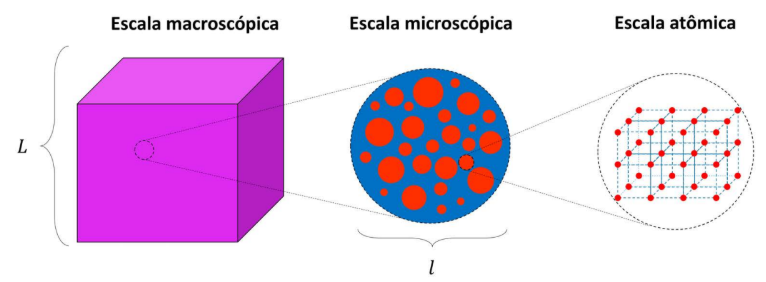
\includegraphics[width=0.75\linewidth]{capitulos/imagens/Separação de escalas.png}
    \caption{Representação esquemática do princípio da separação de escalas e do parâmetro geométrico adimensional $\epsilon$.}
    \label{fig:separacao_escalas}
\end{figure}

A validade física e matemática das abordagens multiescala repousa sobre a condição $0 < \epsilon \ll 1$. Quando o parâmetro $\epsilon$ é suficientemente pequeno, torna-se possível desacoplar os problemas nas duas escalas espaciais: a coordenada macroscópica lenta $\mathbf{x}$ e a coordenada microscópica rápida $\mathbf{y} = \mathbf{x}/\epsilon$, responsável por descrever as oscilações periódicas locais da solução dentro da célula unitária \cite{bakhvalov1989}. 

Para a condução da modelagem analítica, postula-se uma \textit{Solução Assintótica Formal} (SAF) expressa como uma série de potências do parâmetro $\epsilon$: (conforme desenvolvido no Capítulo 3, Seção 3.2).
\begin{equation}
  \mathbf{u}^{(\infty)}(\mathbf{x}, \epsilon) = \mathbf{u}^0(\mathbf{x}) + \epsilon \mathbf{u}^1(\mathbf{x}, \mathbf{y}) + \epsilon^2 \mathbf{u}^2(\mathbf{x}, \mathbf{y}) + \dots
  \label{eq:saf_expansao}
\end{equation}

A substituição desta expansão nas equações governantes de equilíbrio mecânico e a segregação dos termos por ordens de magnitude em $\epsilon$ decompõem o problema original em uma hierarquia bem definida:
\begin{enumerate}
    \item Um \textit{problema local sobre a célula unitária}, que fornece as funções de perturbação elástica e permite calcular de forma analítica fechada os \textbf{coeficientes elásticos efetivos} do cilindro homogeneizado;
    \item Um \textit{problema macroscópico equivalente}, formulado sobre o domínio contínuo global e governado pelas propriedades homogeneizadas.
\end{enumerate}

No formalismo do MHA, a aproximação de ordem zero ($\mathbf{u}^0$) descreve com precisão a resposta macroscópica média de deslocamentos da estrutura. O termo corretor de primeira ordem $\epsilon \mathbf{u}^1(\mathbf{x}, \mathbf{y})$, por sua vez, é responsável por capturar as flutuações e os gradientes locais decorrentes da heterogeneidade. No presente trabalho, a formulação analítica do MHA é desenvolvida até a determinação fechada das propriedades constitutivas efetivas e a resolução do campo macroscópico $\mathbf{u}^0$, enquanto a implementação computacional da reconstrução analítica ponto a ponto das flutuações locais via $\epsilon \mathbf{u}^1$ é delineada formalmente como etapa de extensão em trabalhos futuros, sendo a validação dos campos locais conduzida comparativamente frente ao modelo detalhado em elementos finitos.

\section{Objetivo geral}

O objetivo geral deste trabalho é realizar uma análise mecânica multiescala de vasos de pressão cilíndricos multicamadas com periodicidade radial, estabelecendo uma comparação sistemática e quantitativa de precisão e eficiência computacional entre o Método dos Elementos Finitos (MEF), empregado como modelo detalhado de referência, e o Método de Homogeneização Assintótica (MHA), empregado como formulação analítica equivalente, tendo a clássica solução analítica exata de Lamé como padrão fundamental de calibração e verificação do solucionador numérico para o caso homogêneo.

\section{Objetivos específicos}

Para atingir o objetivo geral, definem-se os seguintes objetivos específicos:

\begin{enumerate}
  \item \textbf{Formular o problema de equilíbrio mecânico do cilindro compósito microperiódico} em coordenadas cilíndricas tridimensionais sob hipótese de simetria de revolução (axissimetria) e deformação plana generalizada, deduzindo a equação diferencial ordinária governante unidimensional radial;
  \item \textbf{Aplicar o formalismo do MHA ao problema formulado}, deduzindo as equações diferenciais recorrentes, as condições de contorno de célula unitária, as funções corretoras locais e a equação governante homogeneizada macroscópica;
  \item \textbf{Deduzir analiticamente os coeficientes elásticos efetivos} para a configuração cilíndrica bilaminada bimetálica (aço--alumínio), correlacionando os resultados obtidos com os limites clássicos de Reuss (média harmônica radial) e a formulação de meios estratificados de Backus (rigidez circunferencial e módulo de cisalhamento efetivo);
  \item \textbf{Implementar e calibrar um solucionador numérico axissimétrico} baseado na plataforma de elementos finitos em código aberto FEniCS, validando a formulação variacional fraca através da clássica solução analítica de Lamé para cilindros homogêneos de parede grossa;
  \item \textbf{Comparar quantitativamente a precisão e a eficiência computacional} entre a solução macroscópica homogeneizada pelo MHA e a solução numérica detalhada do MEF, avaliando o comportamento assintótico das descontinuidades de gradiente nas interfaces, a redução dos erros numéricos e o ganho de tempo de processamento (\textit{speedup}) em função do aumento do número de camadas do vaso.
\end{enumerate}

\section{Organização e limitações do trabalho}

O presente trabalho está estruturado em seis capítulos:
\begin{itemize}
    \item O \textbf{Capítulo 1 (Introdução)} contextualiza a pesquisa, justifica a seleção dos materiais e estabelece os objetivos e delimitações do estudo;
    \item O \textbf{Capítulo 2 (Revisão Bibliográfica)} aborda os critérios normativos para vasos de pressão (ASME Seção VIII e NR-13), a mecânica dos materiais compósitos anisotrópicos, as teorias cinemáticas de placas/cascas, os mecanismos de descontinuidade em interfaces e os fundamentos do MHA e do MEF;
    \item O \textbf{Capítulo 3 (Formulação Matemática e Homogeneização)} apresenta o equacionamento analítico do equilíbrio axissimétrico em coordenadas cilíndricas e desenvolve a dedução detalhada do MHA e dos coeficientes constitutivos efetivos;
    \item O \textbf{Capítulo 4 (Metodologia e Simulação Numérica)} descreve a implementação computacional do modelo de elementos finitos axissimétrico no ambiente FEniCS, detalhando a discretização da malha estruturada, as funções de interpolação e o mapeamento periódico das propriedades mecânicas;
    \item O \textbf{Capítulo 5 (Resultados e Discussões)} expõe a validação analítica via solução de Lamé, a análise comparativa de deslocamentos e tensões entre MEF e MHA, o comportamento assintótico de convergência e a avaliação de eficiência computacional e alívio de peso estrutural;
    \item O \textbf{Capítulo 6 (Conclusões e Trabalhos Futuros)} sintetiza as principais contribuições técnicas do estudo e delineia propostas para extensões da pesquisa.
\end{itemize}

\subsection{Delimitação do escopo e limitações do modelo}

A fim de assegurar o rigor e a consistência da modelagem matemática e numérica desenvolvida, o escopo deste trabalho está delimitado sob as seguintes premissas e simplificações físicas:
\begin{itemize}
    \item \textbf{Regime mecânico e cinemático:} Considera-se comportamento elástico linear, puramente isotrópico em nível de subcamada homogênea individual, operando sob a hipótese de deformações e deslocamentos infinitesimais;
    \item \textbf{Condição cinemática de extremidade:} Adota-se o estado de deformação plana generalizada ($\epsilon_{zz} = \text{constante}$), condizente com cilindros de comprimento axial longo submetidos a carregamento uniforme de pressão interna de regime permanente ($P_{\text{int}} = 30 \, \text{MPa}$);
    \item \textbf{Condições interfaciais ideais:} Assume-se aderência e contato mecânico perfeito entre as lâminas adjacentes de aço e alumínio, com continuidade estrita de deslocamentos radiais e tensões de tração normais, desconsiderando fenômenos de delaminação, escorregamento interfacial, plasticidade ou propagação de trincas;
    \item \textbf{Condições térmicas e ambientais:} A análise é estritamente isotérmica, desconsiderando efeitos de gradientes de temperatura, dilatação térmica diferencial residual de fabricação ou mecanismos de corrosão galvânica entre as fases metálicas;
    \item \textbf{Alcance da implementação do MHA:} O modelo de homogeneização analítico é aplicado à dedução das constantes constitutivas efetivas e à resolução da resposta macroscópica de deslocamento médio ($\mathbf{u}^0$), sendo a implementação numérica computacional da reconstrução pós-processada ponto a ponto do campo local corretivo ($\epsilon \mathbf{u}^1$) reservada para investigações e trabalhos futuros.
\end{itemize}


% Revisão Bibliográfica
 \chapter{Revisão Bibliográfica}

\section{Vasos de Pressão e Critérios Normativos}

\subsection{Classificação Geométrica: Paredes Finas vs. Paredes Grossas}

Sob o ponto de vista da mecânica do contínuo e da resistência dos materiais, o dimensionamento elástico e a distribuição de tensões ao longo da parede do vaso são intrinsecamente dependentes da relação geométrica entre o raio interno ($r$) e a espessura da parede ($t$). Por este motivo, a literatura clássica estabelece o seguinte critério de classificação estrutural:

\textbf{Vasos de Parede Fina:} Ocorrem quando a relação geométrica satisfaz a desigualdade:

$\frac{r}{t} \ge 10.$ \label{eq-limite-parede-fina}

Nesta condição, assume-se que as tensões normais de tração atuantes na parede do vaso são uniformes ao longo de toda a espessura, sendo chamadas de tensões de membrana \cite[p.~415]{asme_sec8_div1_2019}.

\textbf{Vasos de Parede Grossa:} Ocorrem quando a espessura do vaso é expressiva ($r/t < 10$), fazendo com que a distribuição de tensões varie radialmente de forma não linear ao longo da espessura, exigindo o emprego de soluções completas de elasticidade (como as clássicas soluções de Lamé) devido ao alto gradiente de tensões e efeitos de cisalhamento interlaminar \cite[p.~591]{Sadd2009}.

A \cite[p.~19]{asme_sec8_div1_2019} cita também que as duas geometrias primárias mais difundidas na indústria para a contenção de fluidos pressurizados são os cilindros (verticais ou horizontais) e as esferas. Para reservatórios cilíndricos de parede fina sujeitos a uma pressão manométrica interna $p$, \cite[p.~159]{Sadd2009} afirma que o estado plano de tensões é governado por tensões principais normais sem componentes de cisalhamento, devido à simetria axial (axissimetria) do cilindro e do carregamento. \cite[p.~652]{beer1989resistencia} deduzem a tensão circunferencial (ou tangencial/hoop), denotada por $\sigma_1$, que atua no sentido tangencial ao longo do costado cilíndrico, sendo expressa como:

$\sigma_1 = \frac{p \, r}{t}.$ \label{eq-tensao-circunferencial}

De modo similar, a tensão longitudinal (ou axial), denotada por $\sigma_2$, atua paralelamente ao eixo do cilindro e é gerada pelas forças de pressão que empurram os tampões de extremidade, sendo descrita por \cite{beer1989resistencia}

$\sigma_2 = \frac{p \, r}{2 \, t}.$ \label{eq-tensao-longitudinal}


Em contrapartida, para reservatórios esféricos de parede fina, \cite[p.~652]{beer1989resistencia} ressaltam que a perfeita simetria esférica do domínio faz com que as tensões circunferenciais e longitudinais sejam idênticas ($\sigma_1 = \sigma_2$), resultando em:

$ \sigma_1 = \sigma_2 = \frac{pr}{2t} $ <eq-tensao-esferica>

No estado de tensões na parede de uma esfera, as tensões principais normais são iguais, o que faz com que o círculo de Mohr correspondente ao plano tangencial se reduza a um único ponto, zerando a tensão cisalhante máxima no plano ($\tau_{\text{no plano}} = 0$). No entanto, a tensão cisalhante máxima absoluta (fora do plano) para cilindros e esferas é dada, respectivamente, por \cite[p.~656]{beer1989resistencia}:

\begin{equation}
  \begin{aligned}
    \tau_{\max,\text{cilindro}} &= \frac{\sigma_1}{2} = \frac{p \, r}{2 \, t} \\
    \tau_{\max,\text{esfera}} &= \frac{\sigma_1}{2} = \frac{p \, r}{4 \, t}
  \end{aligned}
\end{equation}

Essa distribuição de tensões prova que, embora os vasos esféricos apresentem uma fabricação muito mais complexa e cara devido à necessidade de conformação tridimensional de gomos soldados, eles são mecanicamente muito mais eficientes, sendo capazes de suportar o dobro de pressão interna em relação a um vaso cilíndrico de mesmo diâmetro e espessura.

\subsection{Gestão de Segurança e Integridade Estrutural Conforme a NR-13}

No Brasil, a operação e integridade física de todos os vasos de pressão industriais são regulamentadas de forma obrigatória pela Norma Regulamentadora \cite{brasil_nr13_2022}, intitulada "Caldeiras, Vasos de Pressão, Tubulações e Tanques Metálicos de Armazenamento". A NR-13 estabelece requisitos mínimos legais para a gestão da integridade estrutural desses equipamentos nos aspectos relacionados à instalação, inspeção de segurança, operação e manutenção, visando prioritariamente prevenir acidentes severos e resguardar a vida dos trabalhadores.

Conforme definido pela norma NR-13, vasos de pressão são conceitualmente definidos como quaisquer recipientes estanques, independentemente de sua geometria, dimensões ou finalidade, capazes de conter um fluido sob pressão positiva ou negativa (vácuo) significativamente diferente da pressão atmosférica.

% Na engenharia de processos e segurança do trabalho, conforme definido pela \cite[p.~2]{asme_sec8_div1_2019} adota-se um divisor clássico para diferenciar esses equipamentos de simples reservatórios de armazenamento: quando a diferença de pressão interna e externa é superior a $0.1$ MPa (ou aproximadamente $15$ psig ou $1.0$ bar), o equipamento é enquadrado e projetado como um vaso de pressão; para diferenciais de pressão inferiores a esse patamar, a estrutura é classificada como um tanque de armazenamento.

A norma possui critérios bem delineados de abrangência de fiscalização para enquadramento de recipientes sob suas regras. Conforme o subitem 13.2.1, estão inclusos no escopo da NR-13 \cite{brasil_nr13_2022}:

1. Vasos de pressão cujo produto entre a pressão máxima de operação ($P$, em kPa) e seu volume interno ($V$, em m³) seja superior a 8 ($P.V > 8$) \cite{brasil_nr13_2022};
2. Vasos de pressão que contenham fluidos de Classe A (fluidos altamente tóxicos, inflamáveis ou hidrogênio), independentemente do valor do produto $P.V$ \cite{brasil_nr13_2022}.

Por outro lado, recipientes com diâmetro interno inferior a $150$ mm estão formalmente dispensados da aplicação da norma, independentemente do fluido ou pressão de operação \cite{brasil_nr13_2022}.

A NR-13 organiza os vasos de pressão em categorias de risco (de I a V, onde a Categoria I representa a classe de risco mais elevado e a Categoria V o menor risco), as quais regulam diretamente a periodicidade máxima permitida para as inspeções de segurança internas e externas e testes de integridade \cite{brasil_nr13_2022}. Essa categorização é definida em função de dois parâmetros principais: a \textbf{Classe de Fluido} e o \textbf{Grupo de Potencial de Risco} \cite{brasil_nr13_2022}.

\textbf{Classes de Fluido (Subitem 13.5.1.1.1):}Os fluidos de processo contidos nos vasos de pressão são classificados em quatro classes distintas com base em sua inflamabilidade, toxicidade e reatividade \cite{brasil_nr13_2022}:

\begin{itemize}
  \item \textbf{Classe A:} Fluidos inflamáveis; combustíveis com temperatura de operação igual ou superior a $200$ ºC; fluidos tóxicos com limite de tolerância igual ou inferior a $20$ ppm; hidrogênio e acetileno \cite{brasil_nr13_2022}.
  \item \textbf{Classe B:} Fluidos combustíveis com temperatura de operação inferior a $200$ ºC; fluidos tóxicos com limite de tolerância superior a $20$ ppm \cite{brasil_nr13_2022}.
  \item \textbf{Classe C:} Vapor de água; gases asfixiantes simples; ar comprimido \cite{brasil_nr13_2022}.
  \item \textbf{Classe D:} Outros fluidos não enquadrados nas classes anteriores (como água potável ou fluidos inertes) \cite{brasil_nr13_2022}.
\end{itemize}

\textbf{Grupo de Potencial de Risco (Subitem 13.5.1.1.3):} Estabelecido a partir do produto matemático $P.V$, onde $P$ é o módulo da pressão máxima de operação em megapascais ($"MPa"$) e $V$ é o volume interno do vaso em metros cúbicos ($"m"^3$), divididos nos seguintes cinco grupos \cite{brasil_nr13_2022}:
\begin{itemize}
  \item \textbf{Grupo 1:} $P.V \ge  100$ \cite{brasil_nr13_2022};
  \item \textbf{Grupo 2:} $100 > P.V \ge  30$ \cite{brasil_nr13_2022};
  \item \textbf{Grupo 3:} $30 > P.V \ge  2,5$ \cite{brasil_nr13_2022};
  \item \textbf{Grupo 4:} $2,5 > P.V \ge  1$ \cite{brasil_nr13_2022};
  \item \textbf{Grupo 5:} $P.V < 1$ \cite{brasil_nr13_2022}.
\end{itemize}

Cruzando-se as matrizes de Classe de Fluido com o Grupo de Potencial de Risco, a Tabela 1 da NR-13 define formalmente a Categoria do Vaso de Pressão \cite{brasil_nr13_2022}:


Conforme a Subseção A, Parte UG do ASME Seção VIII Divisão 1, as fórmulas utilizadas para o cálculo da espessura mínima requerida ($t$) e da Pressão Máxima de Trabalho Admissível (PMTA, ou $P$) de cascos cilíndricos sob pressão interna são baseadas na tensão circunferencial solicitando as juntas soldadas longitudinais \cite{asme_sec8_div1_2019}. Quando a espessura do costado não excede a metade do raio interno, ou quando a pressão interna não ultrapassa o limite elástico $0,385 S E$, aplicam-se as seguintes expressões de projeto (UG-27) \cite{asme_sec8_div1_2019}:
$t = \frac{P \, R}{S \, E - 0{,}6 \, P} \quad \text{ou} \quad P = \frac{S \, E \, t}{R + 0{,}6 \, t}$ \label{eq-asme-circunferencial}

Onde:

\begin{itemize}
  \item $t$ é a espessura mínima de parede requerida (excluindo sobrespessuras de corrosão), em milímetros ($"mm"$) \cite{asme_sec8_div1_2019};
  \item $P$ é a pressão interna de projeto ou a PMTA, em megapascais ($"MPa"$) \cite{asme_sec8_div1_2019};
  \item $R$ é o raio interno do casco cilíndrico na condição corroída, em milímetros ($"mm"$) \cite{asme_sec8_div1_2019};
  \item $S$ é o valor máximo da tensão de tração admissível do material na temperatura de projeto, obtido nas tabelas da Seção II Parte D do Código ASME, em megapascais ($"MPa"$) \cite{asme_sec8_div1_2019};
  \item $E$ é a eficiência de junta soldada circunferencial ou longitudinal, que varia de $0,70$ a $1,00$ em função da extensão dos exames radiográficos realizados na junta (conforme parágrafos UW-11 e UW-12) \cite{asme_sec8_div1_2019}.
\end{itemize}

Para as juntas circunferenciais solicitadas pela tensão longitudinal, sob as mesmas condições geométricas de parede fina (espessura menor que metade do raio interno e $P \le  1,25 S E$), as equações do parágrafo UG-27 do ASME Seção VIII Div. 1 resultam em \cite{asme_sec8_div1_2019}:
$t = \frac{P \, R}{2 \, S \, E + 0{,}4 \, P} \quad \text{ou} \quad P = \frac{2 \, S \, E \, t}{R - 0{,}4 \, t}$ \label{eq-asme-longitudinal}

O código estabelece de forma rigorosa que a espessura mínima nominal a ser adotada para a fabricação de cascos e tampos de aço carbono e baixa liga, independentemente do cálculo por pressão, é o maior valor entre $4,8$ mm ou a relação baseada no diâmetro interno com tolerância à corrosão (UG-16), visando garantir estabilidade dimensional e facilidade de fabricação na caldeiraria \cite{asme_sec8_div1_2019}.
% ====================================================

\section{Mecânica dos Materiais Compósitos e Simetrias Elásticas (Objetivo B.2)}

O estudo do comportamento mecânico de estruturas cilíndricas multicamadas e vasos de pressão avançados requer uma base conceitual sólida da mecânica dos meios anisotrópicos. Ao contrário dos materiais convencionais, cuja isotropia simplifica as relações constitutivas, os compósitos exibem propriedades físicas que dependem da direção analisada. Esta seção apresenta o formalismo matemático da Lei de Hooke Generalizada, o método de redução de constantes elásticas através das simetrias elásticas e a Notação de Voigt, culminando na justificativa física de como cilindros formados por camadas isotrópicas apresentam um comportamento macroscopicamente ortotrópico curvilíneo \cite{RMJones2018}.

\subsection{Lei de Hooke Generalizada e o Tensor de Rigidez de Quarta Ordem}

No âmbito da elasticidade linear tridimensional, a relação entre o tensor de tensões de segunda ordem $\mathbf{\sigma}$ e o tensor de deformações infinitesimais de segunda ordem $\mathbf{\epsilon}$ é regida pela Lei de Hooke Generalizada, expressa em notação de índices como \cite{lai2010continuum}:

\begin{equation} 
    \sigma_{ij} = C_{ijkl} \epsilon_{kl} , \quad (i, j, k, l = 1, 2, 3),
\end{equation}\label{eq:hooketensor}

onde $C_{ijkl}$ representa o tensor de elasticidade (ou rigidez elástica) de quarta ordem. De acordo com a análise dimensional e a álgebra tensorial, o tensor $C_{i j k l}$ possui $3^4 = 81$ componentes independentes na ausência de simetrias \cite{lai2010continuum}.

O tensor de deformações infinitesimais $\mathbf{\epsilon}$ é definido como a parte simétrica do gradiente do campo de deslocamentos $\mathbf{u}$, ou seja, $\epsilon_{ij} = \frac{1}{2}(u_{i,j} + u_{j,i})$, onde $u_{i,j} = \partial u_i / \partial x_j$ denota a derivada parcial do componente $i$ do deslocamento em relação à coordenada $j$ \cite{lai2010continuum, Sadd2009}. O gradiente do vetor deslocamento $\nabla \mathbf{u}$ é o tensor de segunda ordem cujas componentes são $u_{i,j}$; sua parte antissimétrica corresponde à rotaçãoo infinitesimal do meio, de modo que apenas a parte simétrica (a deformaçao) contribui para o trabalho de deformação elástica.

Contudo, a física dos meios contínuos impõe restrições severas a essas componentes devido às simetrias físicas dos tensores de tensão e deformação, bem como a princípios termodinâmicos \cite{lai2010continuum}:

1. \textbf{Simetria do Tensor de Tensões:} Em virtude da conservação do momento angular (e na ausência de momentos de corpo distribuídos), o tensor de tensões de Cauchy é simétrico ($\sigma_{(ij)} = \sigma_{(ji)}$). Isto resulta na simetria menor esquerda do tensor de rigidez \cite{Sadd2009}:

$ C_{ijkl} = C_{jikl} $ \label{eq:sym_left}

2. \textbf{Simetria do Tensor de Deformações:} Por definição cinemática, o tensor de pequenas deformações é a parte simétrica do gradiente do vetor deslocamento ($\epsilon_{(kl)} = \frac{1}{2}(u_{(k,l)} + u_{(l,k)})$). Isto implica na simetria menor direita \cite{Sadd2009}:

$ C_{ijkl} = C_{ijlk} $ \label{eq:sym_right}

A aplicação conjunta das simetrias menores dadas pelas \eqref{eq:sym_left} e \eqref{eq:sym_right} reduz o número de componentes elásticas independentes de 81 para 36 componentes \cite{lai2010continuum}.

3. \textbf{Existência de um Potencial Elástico (Termodinâmica):} Para um material elástico hiperelástico, assume-se a existência de uma função de densidade de energia de deformação (ou potencial elástico $W$) por unidade de volume, de modo que as tensões sejam derivadas de $W$ por \cite{Timoshenko_1951}:
  $ \sigma_{(ij)} = \frac{\partial W}{\partial \epsilon_{(ij)}} $ \label{eq:potential_w}

Diferenciando novamente a expressão anterior em relação às deformações, obtêm-se as componentes de rigidez \cite{lai2010continuum}:

$ C_{ijkl} = \frac{\partial^2 W}{\partial \epsilon_{(ij)} \partial \epsilon_{(kl)}} $ \label{eq:stiff_deriv}

Como a ordem de diferenciação parcial de uma função contínua de classe $C^2$ é imaterial (teorema de Clairaut-Schwarz), conclui-se que o tensor de rigidez possui simetria maior \cite{lai2010continuum}:
$ C_{ijkl} = C_{klij} $ \label{eq:sym_major}

A introdução da simetria maior dada pela \eqref{eq:sym_major} impõe que a matriz elástica resultante seja simétrica, reduzindo o número máximo de constantes elásticas independentes para o caso de um material elástico anisotrópico tridimensional geral (triclínico) para exatamente \textbf{21 componentes} \cite{Timoshenko_1951}.

\subsection{Notação de Voigt e a Redução Matricial 6x6}

Com o intuito de simplificar a manipulação algébrica e a implementação computacional, utiliza-se a Notação de Voigt para contrair os tensores de segunda e quarta ordens em arranjos matriciais de menor dimensão \cite{Sadd2009}. A contração de índices segue o algoritmo padrão de mapeamento para os índices de tensão e deformação normais e cisalhantes :

\begin{table}[htbp]
\centering
\caption{Notacao de Voigt: correspondencia entre indices tensoriais e de Voigt.}
\label{tab:voigt_notation}
\begin{tabular}{c c c c}
\hline
\textbf{Indice Tensorial $(ij)$} & \textbf{Indice de Voigt $(\alpha)$} & \textbf{Tensao Voigt ($\sigma_\alpha$)} & \textbf{Deformacao Voigt ($\epsilon_\alpha$)} \\ \hline
$11$ & $1$ & $\sigma_1 = \sigma_{11}$ & $\epsilon_1 = \epsilon_{11}$ \\
$22$ & $2$ & $\sigma_2 = \sigma_{22}$ & $\epsilon_2 = \epsilon_{22}$ \\
$33$ & $3$ & $\sigma_3 = \sigma_{33}$ & $\epsilon_3 = \epsilon_{33}$ \\
$23$ ou $32$ & $4$ & $\sigma_4 = \tau_{23}$ & $\epsilon_4 = \gamma_{23} = 2\epsilon_{23}$ \\
$13$ ou $31$ & $5$ & $\sigma_5 = \tau_{13}$ & $\epsilon_5 = \gamma_{13} = 2\epsilon_{13}$ \\
$12$ ou $21$ & $6$ & $\sigma_6 = \tau_{12}$ & $\epsilon_6 = \gamma_{12} = 2\epsilon_{12}$ \\ \hline
\end{tabular}
\end{table}

É de extrema importância frisar que, ao contrair o tensor de deformações, introduz-se um fator multiplicador de 2 nas componentes cisalhantes ($\gamma_\alpha = 2\epsilon_{ij}$ para $i \neq  j$), de modo a preservar o trabalho interno virtual $d W = \sigma\textit{(i j) d \epsilon}(i j) = \sigma\textit{\alpha d \epsilon}\alpha$ \cite{Sadd2009}.

Aplicando a notação de Voigt, a Lei de Hooke tridimensional assume a forma matricial \cite{Sadd2009}:

\begin{equation}
  \begin{aligned}
    \begin{bmatrix}
  \sigma_1 \\
  \sigma_2 \\
  \sigma_3 \\
  \tau_{23} \\
  \tau_{13} \\
  \tau_{12}
\end{bmatrix} = \begin{bmatrix}
  C_{11} & C_{12} & C_{13} & C_{14} & C_{15} & C_{16} \\
  C_{12} & C_{22} & C_{23} & C_{24} & C_{25} & C_{26} \\
  C_{13} & C_{23} & C_{33} & C_{34} & C_{35} & C_{36} \\
  C_{14} & C_{24} & C_{34} & C_{44} & C_{45} & C_{46} \\
  C_{15} & C_{25} & C_{35} & C_{45} & C_{55} & C_{56} \\
  C_{16} & C_{26} & C_{36} & C_{46} & C_{56} & C_{66}
\end{bmatrix} \begin{bmatrix}
  \epsilon_1 \\
  \epsilon_2 \\
  \epsilon_3 \\
  \gamma_{23} \\
  \gamma_{13} \\
  \gamma_{12}
\end{bmatrix}
  \end{aligned}
  \label{eq:voigt_matrix_anisotropic}
\end{equation}

A equação \eqref{eq:voigt_matrix_anisotropic} representa a relação constitutiva de um material triclínico genérico, caracterizado por 21 componentes de rigidez elástica independentes e acoplamento total entre deformações normais e tensões cisalhantes (e vice-versa) \cite{Sadd2009}.

\subsection{Classes de Simetria Elástica e Redução de Constantes}

À medida que o material exibe planos de simetria física ou estrutural em sua microestrutura, o número de constantes elásticas independentes é reduzido de forma sistemática através de leis de transformação de coordenadas tensoriais \cite{lai2010continuum}. Três simetrias elásticas são fundamentais para o entendimento do comportamento dos compósitos estruturais:

\subsubsection{Material Monoclínico (1 Plano de Simetria)}
Se o material possui um único plano de simetria elástica (por exemplo, o plano $x_1 - x_2$), as propriedades elásticas devem permanecer invariantes sob uma transformação de reflexão em relação a este plano ($x_3' = -x_3$). Isso anula as constantes de acoplamento cisalhante fora do plano, reduzindo o número total de constantes para \textbf{13 componentes} \cite{RMJones2018}:

\begin{equation}
  \begin{aligned}
    [C] = \begin{bmatrix}
  C_{11} & C_{12} & C_{13} & 0 & 0 & C_{16} \\
  C_{12} & C_{22} & C_{23} & 0 & 0 & C_{26} \\
  C_{13} & C_{23} & C_{33} & 0 & 0 & C_{36} \\
  0 & 0 & 0 & C_{44} & C_{45} & 0 \\
  0 & 0 & 0 & C_{45} & C_{55} & 0 \\
  C_{16} & C_{26} & C_{36} & 0 & 0 & C_{66}
\end{bmatrix}
  \end{aligned}
  \label{eq:monoclinic_stiffness}
\end{equation}

\subsubsection{Material Ortotrópico (3 Planos Ortogonais de Simetria)}
Se o material possui três planos ortogonais de simetria mecânica (como é o caso de fibras orientadas em eixos cartesianos ortogonais), as propriedades constitutivas são simétricas em relação a esses três planos de simetria mutuamente perpendiculares \cite{Sadd2009}. Nesse caso, todos os acoplamentos entre esforços normais e distorções angulares desaparecem na base de coordenadas principais do material (PMC), resultando em apenas \textbf{9 constantes independentes} \cite{Sadd2009}:

\begin{equation}
  \begin{aligned}
    [C] = \begin{bmatrix}
  C_{11} & C_{12} & C_{13} & 0 & 0 & 0 \\
  C_{12} & C_{22} & C_{23} & 0 & 0 & 0 \\
  C_{13} & C_{23} & C_{33} & 0 & 0 & 0 \\
  0 & 0 & 0 & C_{44} & 0 & 0 \\
  0 & 0 & 0 & 0 & C_{55} & 0 \\
  0 & 0 & 0 & 0 & 0 & C_{66}
\end{bmatrix}
  \end{aligned}
  \label{eq:orthotropic_stiffness}
\end{equation}

A relação de deformação-tensão (Lei de Hooke invertida) para materiais ortotrópicos em coordenadas principais é tradicionalmente expressa através de propriedades de engenharia com significado físico direto (Módulos de Young ($E_1, E_2, E_3$), Módulos de Cisalhamento ($G_{12}, G_{13}, G_{23}$) e Coeficientes de Poisson ($\nu_{12}, \nu_{13}, nu_{23}$)) \cite{Sadd2009}:

\begin{equation}
  \begin{aligned}
    \begin{bmatrix}
  \epsilon_1 \\
  \epsilon_2 \\
  \epsilon_3 \\
  \gamma_{23} \\
  \gamma_{13} \\
  \gamma_{12}
\end{bmatrix} = \begin{bmatrix}
  1/E_1 & -\nu_{21}/E_2 & -\nu_{31}/E_3 & 0 & 0 & 0 \\
  -\nu_12/E_1 & 1/E_2 & -\nu_{32}/E_3 & 0 & 0 & 0 \\
  -\nu_13/E_1 & -\nu_23/E_2 & 1/E_3 & 0 & 0 & 0 \\
  0 & 0 & 0 & 1/G_23 & 0 & 0 \\
  0 & 0 & 0 & 0 & 1/G_13 & 0 \\
  0 & 0 & 0 & 0 & 0 & 1/G_12
\end{bmatrix} \begin{bmatrix}
  \sigma_1 \\
  \sigma_2 \\
  \sigma_3 \\
  \tau_{23} \\
  \tau_{13} \\
  \tau_{12}
\end{bmatrix}
  \end{aligned}
  \label{eq:orthotropic_compliance}
\end{equation}

Como a matriz de flexibilidade $[S] = [C]^(-1)$ é necessariamente simétrica ($S_{(\alpha\beta)} = S_{(\beta\alpha)}$), as seguintes equações de reciprocidade (uma generalização da Lei de Betti) devem ser rigorosamente atendidas pelas propriedades elásticas de engenharia \cite{Timoshenko_1951}:

$ \frac{\nu_{(ij)}}{E_i} = \frac{\nu_{(ji)}}{E_j} , \quad \text{para} i, j = 1, 2, 3 $ \label{eq:betti_reciprocity}

\subsubsection{Material Transversalmente Isotrópico (1 Plano de Isotropia)}
Se, em qualquer ponto do meio elástico, existe um plano físico no qual as propriedades elásticas são idênticas em todas as direções de forma rotacional, o material é classificado como transversalmente isotrópico \cite{lai2010continuum}. Tomando o plano $2-3$ como o plano de isotropia elástica (no qual as propriedades são invariantes sob qualquer rotação ao longo do eixo $1$), as componentes de rigidez são reduzidas a apenas \textbf{5 constantes elásticas independentes} \cite{lai2010continuum}:

\begin{equation}
  \begin{aligned}
    [C] = \begin{bmatrix}
  C_{11} & C_{12} & C_{12} & 0 & 0 & 0 \\
  C_{12} & C_{22} & C_{23} & 0 & 0 & 0 \\
  C_{12} & C_{23} & C_{22} & 0 & 0 & 0 \\
  0 & 0 & 0 & \frac{C_{22} - C_{23}}{2}
\end{bmatrix}, 0, 0;
    0, 0, 0, 0, C_{55}, 0;
    0, 0, 0, 0, 0, C_{55}
  )
  \end{aligned}
  \label{eq:transverse_isotropic_stiffness}
\end{equation}

onde o termo de cisalhamento no plano de isotropia é definido pela relação clássica $C_{44} = \frac{1}{2}(C_{22} - C_{23})$, análoga à relação elástica linear de materiais puramente isotrópicos \cite{Sadd2009}.

\subsection{Origem Física do Comportamento Ortotrópico Cilíndrico Macroscópico}

A modelagem de vasos de pressão multicamadas, como cilindros bimetálicos compostos por lâminas delgadas e alternadas de aço carbono e ligas de alumínio, introduz um fenômeno físico-matemático de enorme importância: a \textbf{transição de simetria induzida por homogeneização} \cite{bakhvalov1989}.

Embora cada camada individual que constitui a parede do cilindro exiba um comportamento puramente isotrópico (caracterizado localmente por apenas 2 parâmetros elásticos livres, $E$ e $\nu$) \cite{bakhvalov1989}, o processo de empilhamento periódico ao longo do raio $r$ do vaso e a subsequente homogeneização matemática via Método de Homogeneização Assintótica (MHA) quebram a isotropia global da estrutura \cite{PartonReport}.

\subsubsection{O Princípio de Homogeneização de Backus}
Do ponto de vista físico, um cilindro composto por camadas ultrafinas de propriedades mecânicas alternadas comporta-se de forma idêntica a um meio elástico estratificado periódico de Backus \cite{Backus1962}. Sob a ação de um carregamento mecânico macroscópico, a estrutura apresenta rigidez assimétrica:
\begin{itemize}
  \item Na \textbf{direção radial} (perpendicular às interfaces de camadas), a deformação do conjunto é governada por uma associação de "molas em série" (regida pela média harmônica das propriedades elásticas locais), resultando em um comportamento elástico significativamente mais flexível \cite{Backus1962}.
  \item Nas \textbf{direções circunferencial e axial} (paralelas às interfaces), as camadas deformam juntas sob o mesmo campo macroscópico, caracterizando uma associação de "molas em paralelo" (regida pela média aritmética das propriedades), o que induz uma rigidez mecânica consideravelmente maior \cite{Backus1962}.
\end{itemize}

Este desacoplamento de rigidez induz um comportamento macroscópico equivalente de \textbf{ortotropia cilíndrica} (ou isotropia transversal curvilínea), no qual a direção radial $r$ comporta-se como o eixo normal à simetria elástica, enquanto as direções axial $z$ e tangencial $\theta$ formam o plano macroscópico de isotropia elástica curvilínea \cite{Backus1962}.

Como consequência direta do MHA de camadas isotrópicas coaxiais periódicas, o cilindro homogêneo equivalente macroscópico passa a ser regido por um tensor de elasticidade efetivo $[\hat{\mathcal{C}}]$ contendo exatamente \textbf{5 coeficientes independentes} ($hat(C)\textit{{11}, hat(C)}{22}, hat(C)\textit{{12}, hat(C)}{23}$ e $hat(C)_{55}$), em substituição às propriedades locais rapidamente oscilantes do modelo original \cite{Backus1962}. O alinhamento natural dessas constantes com as coordenadas cilíndricas do costado do vaso ($r, \theta, z$) elimina a necessidade de transformações de coordenadas complexas e simplifica drasticamente o equilíbrio axissimétrico final estudado no TCC \cite{Backus1962}.

\section{Teorias de Deformação de Placas/Cascas e o Efeito Zig-Zag (Objetivo B.3)}

O projeto de vasos de pressão e cascas de parede espessa fabricados em materiais compósitos ou arranjos multicamadas exige teorias cinemáticas capazes de descrever com fidelidade a distribuição de deslocamentos e tensões ao longo da espessura. Esta seção aborda a evolução das formulações cinemáticas clássicas de camada única equivalente, as limitações intrínsecas que as tornam inadequadas para cilindros de parede grossa e o mecanismo físico-matemático que rege o efeito zigue-zague (\textbf{kinks}) nas interfaces das camadas com alto contraste de rigidez elástica \cite{RMJones2018}.

\subsection{Teorias de Camada Única Equivalente (Equivalent Single Layer - ESL)}

As teorias de Camada Única Equivalente (ESL) reduzem o problema tridimensional (3D) de elasticidade para uma formulação bidimensional (2D) aproximada, tratando o laminado heterogêneo como uma placa ou casca homogênea equivalente com propriedades integradas ao longo da espessura $h$ \cite{RMJones2018}. As duas principais teorias deste grupo são a Teoria Clássica de Laminação de Placas (CLT) e a Teoria de Deformação por Cisalhamento de Primeira Ordem (FSDT) \cite{RMJones2018}.

\subsubsection{Teoria Clássica de Laminação de Placas (CLT)}

A Teoria Clássica de Laminação (CLT — \textbf{Classical Lamination Theory}), fundamentada nas hipóteses de Kirchhoff-Love para cascas delgadas, assume que qualquer linha reta originalmente normal à superfície neutra do cilindro permanece \cite{RMJones2018}:
1. Reta após a deformação;
2. Normal à superfície deformada;
3. Inalterada em seu comprimento (extensão vertical nula, $\epsilon_z = 0$).

Sob estas premissas cinemáticas, o campo de deslocamentos axial $u_z$ e circunferencial $u_\theta$ a uma coordenada radial $r$ (adotando a superfície média como referência de espessura $z$) é escrito como \cite{RMJones2018}:

$ u_z(r, \theta, z) = u_z^0(r, \theta) - z \frac{\partial w}{\partial z} $ \label{eq:clt_disp1}
$ u_\theta(r, \theta, z) = u_\theta^0(r, \theta) - z \frac{\partial w}{r \partial \theta} $ \label{eq:clt_disp2}
$ u_r(r, \theta, z) = w(r, \theta) $ \label{eq:clt_disp3}

onde $u_z^0$ e $u_\theta^0$ são os deslocamentos no plano médio e $w$ é o deslocamento radial. A principal implicação física da \eqref{eq:clt_disp1} e \eqref{eq:clt_disp2} é a anulação das deformações por cisalhamento transversal elástico \cite{RMJones2018}:

$ \gamma_{(rz)} = 2\epsilon_{(rz)} = 0, \quad \gamma_{(r\theta)} = 2\epsilon_{(r\theta)} = 0 $ \label{eq:clt_shear}

A ausência de deformação de cisalhamento transversal restringe a aplicabilidade da CLT estritamente a cascas muito finas ($R_"int"/t \ge  10$), uma vez que o erro introduzido ao ignorar a flexibilidade ao cisalhamento se propaga rapidamente para o cálculo de deflexões e frequências naturais à medida que a espessura aumenta \cite{RMJones2018}.

\subsubsection{Teoria de Deformação por Cisalhamento de Primeira Ordem (FSDT)}

Para contornar a rigidez excessiva da CLT, a Teoria de Deformação por Cisalhamento de Primeira Ordem (FSDT — \textbf{First-Order Shear Deformation Theory}), baseada no modelo de Mindlin-Reissner, relaxa a hipótese de normalidade. As seções retas e normais permanecem retas, mas não necessariamente perpendiculares à superfície média após a deformação \cite{RMJones2018}. O campo de deslocamentos é expandido linearmente com a coordenada de espessura $z$ \cite{RMJones2018}:

$ u_z(r, \theta, z) = u_z^0(r, \theta) + z \phi_z(r, \theta) $ \label{eq:fsdt_disp1}
$ u_\theta(r, \theta, z) = u_\theta^0(r, \theta) + z \phi_\theta(r, \theta) $ \label{eq:fsdt_disp2}

onde $\phi_z$ e $\phi_\theta$ representam as rotações das seções transversais em torno dos eixos circunferenciais e axiais. Sob esta formulação, as deformações de cisalhamento transversal são constantes ao longo da espessura \cite{RMJones2018}:

$ \gamma_{(rz)}(z) = \phi_z + \frac{\partial w}{\partial z} = "constante" $ \label{eq:fsdt_shear}

Embora a FSDT capture a flexibilidade global ao cisalhamento, a premissa de deformação cisalhante constante ao longo da espessura viola a condição física de contorno de tensão nula nas superfícies livres superior e inferior do cilindro ($\tau_{(rz)}|(z = p m h/2) = 0$) \cite{RMJones2018}. Na realidade mecânica de um meio homogêneo, a distribuição de tensão de cisalhamento transversal assume um perfil parabólico. Para corrigir essa discrepância energética, a FSDT necessita da introdução de um fator de correção de cisalhamento ($\kappa$), tipicamente adotado como $\kappa = 5/6$ para seções retangulares homogêneas, o qual se torna altamente complexo e impreciso quando aplicado a laminados compostos heterogêneos \cite{RMJones2018}.

\subsection{Limitações de Aplicação em Cilindros de Parede Grossa e Meios de Alto Contraste}

No estudo mecânico de vasos de pressão como o analisado neste trabalho — que apresenta uma espessura de parede $t = 2" mm"$ e raio interno $R_{\text{int}} = 9 \text{ mm}$, resultando em uma relação geométrica de parede grossa $R_{\text{int}}/t = 4,5$ — as teorias de ESL clássicas (CLT e FSDT) tornam-se completamente inadequadas devido a três fatores impeditivos \cite{Sadd2009}:

1. \textbf{Inadmissibilidade de Tensão Radial Nula ($\sigma_{(rr)} = 0$):} Ambas as teorias clássicas de placa assumem um estado plano de tensões, impondo $\sigma_{(rr)} = 0$. Em vasos de parede grossa sob pressão interna $P_i = 10 \text{ MPa}$, a tensão radial $\sigma_{(rr)}$ varia fortemente de $-10" MPa"$ na parede interna até atingir $0$ na face externa, atuando diretamente no escoamento plástico local e nas condições de contorno de equilíbrio \cite{Sadd2009}.
2. \textbf{Ausência do Efeito de Compressibilidade:} As teorias ESL desprezam a deformação normal radial ($\epsilon_{(rr)} = 0$). Em cilindros espessos bimetálicos, o contraste de coeficiente de Poisson induz efeitos de expansão diferencial localizados ao longo do raio que não podem ser negligenciados.
3. \textbf{Omissão das Deformações Interlaminares:} O salto de propriedades mecânicas entre o aço carbono e a liga de alumínio gera altas taxas de cisalhamento interlaminar concentradas junto às interfaces de colagem, fenômeno invisível às abordagens que suavizam as propriedades ao longo da espessura \cite{PartonReport}.

\subsection{O Efeito Zigue-Zague (\textbf{Kinks}) nas Interfaces}

Quando um cilindro ou casca multicamadas é composto por materiais com propriedades elásticas distintas (como o par aço/alumínio), as variáveis elásticas no plano e fora do plano comportam-se de forma descontínua nas interfaces. Esse fenômeno é governado de forma estrita pela mecânica do contato perfeito \cite{RMJones2018}.

Considere a interface perfeitamente aderida entre a camada $k$ e a camada $k+1$ localizada em uma coordenada radial $r = r_k$. As condições físicas de compatibilidade de deslocamento e continuidade de tração (ação e reação) exigem que \cite{RMJones2018}:

$ [[ u_i ]] = u_i^{(k+1)}(r_k) - u_i^{(k)}(r_k) = 0 $ \label{eq:cont_disp}
$ [[ \sigma_{(ri)} ]] = \sigma_{(ri)}^{(k+1)}(r_k) - \sigma_{(ri)}^{(k)}(r_k) = 0, \quad (i = r, \theta, z) $ \label{eq:cont_stress}

A \eqref{eq:cont_disp} impõe que o vetor de deslocamento seja contínuo ao longo de toda a espessura para evitar a abertura de vazios ou o escorregamento entre as fases. Da mesma forma, a \eqref{eq:cont_stress} exige que a tensão normal radial ($\sigma_{(rr)}$) e as tensões de cisalhamento transversal ($\tau_{(rz)}, \tau_{(r\theta)}$) sejam estritamente contínuas na interface para satisfazer o equilíbrio infinitesimal \cite{RMJones2018}.

Contudo, os módulos de elasticidade e cisalhamento das fases sofrem saltos bruscos na transição das camadas (por exemplo, o módulo de cisalhamento do aço é cerca de três vezes superior ao do alumínio, $G_{\text{aço}} \approx 77 \text{ GPa}$ vs $G_{\text{alu}} \approx 26 \text{ GPa}$). Aplicando-se a Lei de Hooke para o cisalhamento transversal, temos \cite{RMJones2018}:

$ \tau_{(rz)} = G(r) \gamma(r z) (r) $ \label{eq:hooke_shear}

Para garantir a continuidade da tens?o de cisalhamento ($\tau_{(rz)}^{(k)} = \tau_{(rz)}^{(k+1)}$) sob a descontinuidade abrupta do m?dulo de cisalhamento ($G^{(k)} \neq G^{(k+1)}$), a deforma??o por cisalhamento transversal ($\gamma_{(rz)}$) obrigatoriamente sofre um salto abrupto na interface \cite{RMJones2018}:

$ [[ \gamma_{(rz)} ]] = \tau_{(rz)}(r_k) \left( \frac{1}{G^{(k+1)}} - \frac{1}{G^{(k)}} \right) \neq 0 $ \label{eq:jump_shear}

Como a deformação por cisalhamento transversal $\gamma_{(rz)}$ é diretamente proporcional à derivada do deslocamento longitudinal em relação ao raio ($\partial_r u_z$), o salto na deformação manifesta-se matematicamente como uma \textbf{descontinuidade na primeira derivada do campo de deslocamentos} ($\partial_r u_i$) \cite{RMJones2018}.

Graficamente, esse fenômeno traduz-se em mudanças súbitas e localizadas de inclinação nas curvas de deslocamento radial ou axial exatamente nos pontos das interfaces elásticas, gerando o formato geométrico de "cotovelos" ou \textbf{"kinks"} conhecido na literatura científica de compósitos laminados como \textbf{comportamento em zigue-zague} (\textbf{zig-zag effect}) \cite{RMJones2018}. As teorias ESL, por assumirem aproximações polinomiais contínuas (C¹-contínuas) de deslocamento ao longo de toda a espessura, são matematicamente incapazes de reproduzir esses kinks elásticos locais, resultando em subestimação severa das deformações interlaminares de cisalhamento \cite{RMJones2018}.

A continuidade da tensão normal radial $\sigma_{rr}$ e das tensões de cisalhamento transversal $\tau_{rz}$, $\tau_{r\theta}$ na interface segue diretamente do \textbf{Lema de Cauchy} (equilíbrio de um tetraedro infinitesimal na superfície de descontinuidade): o vetor de tração $\mathbf{t} = \boldsymbol{\sigma}\cdot\mathbf{n}$ deve ser contínuo através de qualquer superfície, e como a normal $\mathbf{n}$ é a mesma (em módulo) nos dois lados da interface, as componentes de tensão que atuam sobre a normal devem coincidir. Isso é o que permite afirmar que $\sigma_{rr}^{(k)} = \sigma_{rr}^{(k+1)}$ e $\tau_{rz}^{(k)} = \tau_{rz}^{(k+1)}$ na interface $r = r_k$, mesmo quando o módulo de cisalhamento $G$ sofre salto \cite{Sadd2009}.

\subsection{Teorias Camada a Camada (\textbf{Layerwise}) e Teorias Zigue-Zague (ZZT)}

Para representar com precisão física o efeito zigue-zague sem recorrer a simulações elásticas tridimensionais (3D) completas de altíssimo custo computacional, foram desenvolvidas formulações cinemáticas avançadas: as Teorias Camada a Camada (\textbf{Layerwise Theories}) e as Teorias Zigue-Zague (ZZT) \cite{PartonReport}.

1. \textbf{Teorias Camada a Camada (Layerwise):} Nesta abordagem, as equações de deslocamento 2D são formuladas de forma independente para cada uma das $N$ camadas do laminado, conectando as variáveis nas interfaces por equações de restrição de continuidade \cite{PartonReport}. Embora extremamente precisas para capturar os "kinks" e as tensões interlaminares de borda livre, as teorias \textbf{layerwise} possuem a severa desvantagem de que o número total de variáveis de deslocamento (graus de liberdade) da estrutura cresce linearmente com o número de camadas ($N$), tornando o método proibitivo para cilindros de múltiplos períodos ou COPVs de dezenas de lâminas.
2. \textbf{Teorias Zigue-Zague (ZZT — Zig-Zag Theories):} As ZZT superam essa limitação ao enriquecer as teorias de camada única equivalente (como a FSDT) através da superposição de uma função em zigue-zague contínua por partes ($zeta_i (z)$) de amplitude variável, de modo a induzir de forma analítica a descontinuidade de derivada desejada nas interfaces \cite{PartonReport}:
  \begin{equation}
  u_z(r, \theta, z) = u_z^0(r, \theta) + z \phi_z(r, \theta) + \sum_{k=1}^{N-1} \zeta_k(z) \hat{\phi}_z^k(r, \theta)
  \label{eq:zzt_disp}
\end{equation}

As funções de enriquecimento $\zeta_k(z)$ são pré-calculadas analiticamente de forma a satisfazer a priori as condições de continuidade de tensões interlaminares na interface (\eqref{eq:cont_stress}). Como resultado prático, as Teorias Zigue-Zague conseguem capturar com precisão cirúrgica os "kinks" nos deslocamentos e prever o início de falhas por delaminação interlaminares mantendo o número total de graus de liberdade do modelo matemático independente do número de camadas do compósito, oferecendo uma excelente alternativa computacional para análises mecânicas locais \cite{PartonReport}.

\subsection{Justificativa para a Adoção da Homogeneização Assintótica (MHA) frente às ZZT}

Embora as Teorias Zigue-Zague (ZZT) representem um avanço cinematográfico significativo ao desacoplar os graus de liberdade globais do número de camadas $N$, a adoção do Método de Homogeneização Assintótica (MHA) se justifica por razões de escalabilidade, rigor matemático e facilidade de implementação numérica no projeto de vasos multicamadas com alto número de períodos \cite{bakhvalov1989}:

1. \textbf{Inviabilidade Algébrica sob Alta Periodicidade:} Nas ZZT, as funções de enriquecimento local $zeta_k (z)$ e os coeficientes de acoplamento precisam ser formulados e pré-calculados analiticamente de interface em interface ($N-1$ interfaces) \cite{bakhvalov1989}. Para cilindros bimetálicos de alta densidade periódica ou estruturas com centenas de microcamadas (em que $N$ cresce consideravelmente), a montagem desse sistema algébrico de enriquecimento torna-se altamente complexa, onerosa e propensa a erros numéricos de condicionamento. O MHA contorna isso completamente ao desacoplar as escalas de análise: o problema físico global é resolvido como um contínuo perfeitamente homogêneo, cuja complexidade matemática é invariante em relação ao número real de camadas \cite{bakhvalov1989}.
2. \textbf{Rigor Matemático e Convergência Provada:} Ao contrário das ZZT, que se baseiam em aproximações cinemáticas ad hoc (ou \textbf{ansatz} físicos), o MHA é ancorado no rigor da análise assintótica clássica e na teoria da $H$-convergência elíptica \cite{bakhvalov1989}. Ele fornece uma prova formal de consistência matemática na qual, por meio do Teorema da Relação de Proximidade em espaços de Sobolev ($L^2$ e $H^1$), a diferença entre a solução heterogênea do MEF e a aproximação homogeneizada decresce de forma estritamente linear com o parâmetro de escala pequena ($\epsilon = l/L -> 0$) \cite{bakhvalov1989}. Isso garante que, quanto maior for a densidade de camadas do vaso, mais exata e robusta é a resposta fornecida pelo MHA.
3. \textbf{Acoplamento Direto e Simplicidade em Solvers de Elementos Finitos (FEniCS):} A implementação numérica de elementos finitos enriquecidos baseados em ZZT exige o desenvolvimento de elementos customizados não padronizados e formulações variacionais complexas (geralmente indisponíveis em pacotes de MEF comerciais ou open-source) \cite{logg2012automated}. Por outro lado, o MHA permite utilizar elementos lagrangeanos quadráticos clássicos em malhas bidimensionais axissimétricas comuns. O solver do FEniCS resolve o equilíbrio global sem qualquer modificação em suas matrizes de rigidez elástica homogêneas nativas, e o problema de célula local (1D) é resolvido de forma independente e direta, simplificando enormemente a programação e estabilidade numérica do código \cite{logg2012automated}.
4. \textbf{Capacidade de Reconstrução de Campos Locais e Interlaminares:} Uma das maiores vantagens do MHA é o seu caráter de modelagem multiescala bidirecional. Após obter a solução macroscópica homogeneizada suave $u_0(r)$, o comportamento local em zigue-zague dos deslocamentos e as flutuações das tensões interlaminares em cada camada individual podem ser reconstruídos com exatidão analítica a posteriori em qualquer ponto através dos corretores locais elásticos (incluindo a função de perturbação local $N_1(y)$) \cite{bakhvalov1989}:
  $ u_i^\epsilon(r) \approx u_{0,i}(r) + \epsilon N_{1,ij}(y) \frac{\partial u_{0,j}}{\partial r} $ \label{eq:correction_mha}
  Dessa forma, o MHA recupera toda a física microscópica e as descontinuidades de derivada ("kinks") na interface sem sobrecarregar a cinemática global da estrutura \cite{bakhvalov1989}.

\section{Métodos de Homogeneização e a Transição Micro-Macro (Objetivo B.4)}

Conforme discutido na Seção 2.2 (Origem Física do Comportamento Ortotrópico Cilíndrico Macroscópico), o empilhamento periódico de camadas isotrópicas induz ortotropia macroscópica via médias de Backus e os limites clássicos de Voigt e Reuss. A presente seção formaliza matematicamente esses conceitos e apresenta o formalismo do Método de Homogeneização Assintótica (MHA).

A modelagem de materiais heterogêneos com microestrutura complexa impõe desafios severos à análise mecânica clássica. A presença de fases distintas com propriedades mecânicas discrepantes resulta em coeficientes elétricos ou elásticos que oscilam de forma extremamente rápida na escala microscópica. Resolver as equações de equilíbrio elástico em domínios dessa natureza por meio de técnicas discretas diretas, como o Método dos Elementos Finitos (MEF), exige um refinamento de malha tão severo que o custo computacional torna-se proibitivo para estruturas de escala industrial \cite{bakhvalov1989}. Esta seção aborda a transição conceitual e matemática entre as escalas micro e macro, apresentando os limites elásticos clássicos, o modelo de médias de Backus para estratificados e o formalismo rigoroso do Método de Homogeneização Assintótica (MHA).

\subsection{Abordagens Clássicas de Homogeneização e Limites Elásticos}

Historicamente, o problema de determinar propriedades físicas efetivas para meios heterogêneos remonta a trabalhos fundamentais de Poisson, Maxwell, Rayleigh, Voigt e Reuss \cite{PartonReport}. No campo da mecânica dos sólidos, duas formulações fundamentais baseadas em médias volumétricas simples consolidaram-se como balizas analíticas:

1. \textbf{Abordagem de Voigt (Média Aritmética):} Assume que o campo de deformações é perfeitamente uniforme em todo o composto (hipótese de isodeformação ou \textit{isostrain}). A rigidez efetiva equivalente $C_(i j)^V$ é calculada diretamente como a média aritmética ponderada pelas frações volumétricas das fases constituintes:
  $ C_{(ij)}^V = \langle C_{(ij)}(y) \rangle = \sum_{k=1}^{N} V_k C_{(ij)}^{(k)} $ \label{eq:voigt_mean}
  onde $V_k$ representa a fração volumétrica da fase $k$ e $C_{(ij)}^{(k)}$ seu respectivo coeficiente elástico. Termodinamicamente, o modelo de Voigt estabelece o limite superior absoluto para a rigidez do composto \cite{bakhvalov1989}.

2. \textbf{Abordagem de Reuss (Média Harmônica):} Assume que o campo de tensões é uniforme ao longo de todo o domínio (hipótese de isotensão ou \textit{isostress}). A compliância efetiva equivalente $S_(i j)^R$ (inverso da rigidez) é expressa como a média ponderada das compliâncias locais:
  \begin{equation}
  S_{(ij)}^R = \langle S_{(ij)}(y) \rangle = \sum_{k=1}^{N} V_k S_{(ij)}^{(k)} \quad \Leftrightarrow \quad C_{(ij)}^R = \langle C_{(ij)}^{-1}(y) \rangle^{-1}
  \label{eq:reuss_mean}
\end{equation}
  A média de Reuss representa o limite inferior elástico da estrutura heterogênea \cite{bakhvalov1989}.

A diferença entre os limites de Voigt e Reuss é conhecida na literatura micromecânica como o \textbf{Garfo de Hill} (\textit{Hill's fork}) \cite{PartonReport}. Em materiais compósitos com alto contraste de rigidez entre as fases (como o par aço-alumínio ou fibra de carbono e resina epóxi), a distância entre os limites elásticos superior e inferior torna-se demasiadamente larga, de forma que as estimativas médias clássicas perdem a utilidade prática para o projeto estrutural de precisão. Isto justifica a necessidade de métodos matemáticos mais rigorosos, capazes de resolver as equações de célula local de forma exata.

\subsection{Homogeneização de Meios Estratificados e a Média de Backus}

A formulação de Backus (1962) para meios estratificados, introduzida na Seção 2.2, é apresentada a seguir em detalhe analítico, com a dedução das médias harmônicas (Reuss) para a direção transversal e das médias aritméticas corrigidas (Voigt modificado) para as direções paralelas.

Para estruturas compostas por camadas paralelas alternadas de materiais isotrópicos, George Backus (1962) deduziu uma formulação analítica exata que descreve o comportamento macroscópico equivalente de ondas elásticas de longo comprimento \cite{Backus1962}. O modelo de Backus prova matematicamente que o empilhamento periódico de duas fases isotrópicas resulta em um meio macroscópico equivalente com comportamento \textbf{Transversalmente Isotrópico} \cite{Backus1962}.

As equações de Backus misturam médias harmônicas (Reuss) para a direção perpendicular às interfaces e médias aritméticas com correções do efeito de Poisson (Voigt modificado) para as direções paralelas ao plano das camadas \cite{Backus1962}:
\textbf{Direção Transversal (Radial $r$):} O comportamento mecânico é dominado por tensões que atravessam as interfaces, assemelhando-se a molas em série. Portanto, a rigidez efetiva radial transversal é ditada pelo limite de Reuss:
$ \hat{C}_{11} = \langle C_{11}^{-1}(y) \rangle^{-1} $ \label{eq:backus_c11}
\textbf{Direções Paralelas (Circunferencial $\theta$ e Axial $z$):} Como as camadas estão confinadas e ligadas rigidamente, elas deformam-se conjuntamente sob tração paralela (molas em paralelo). A rigidez efetiva circunferencial $C_(22)$ é expressa como uma média aritmética corrigida pelo acoplamento de Poisson das fases \cite{Backus1962}:
\begin{equation}
\hat{C}_{22} = \langle C_{22}(y) \rangle - \langle \nu(y) \rangle^2 \langle C_{11}^{-1}(y) \rangle^{-1}
  \label{eq:backus_c22}
\end{equation}

Sob a ótica do Método de Homogeneização Assintótica (MHA), quando o número de camadas concêntricas periódicas de um vaso de pressão cilíndrico aumenta substancialmente, a espessura de cada lâmina torna-se minúscula frente ao raio global ($\epsilon \to 0$). Nesse limite assintótico, a curvatura local do cilindro desaparece, de modo que a célula unitária anular microscópica comporta-se localmente como um laminado plano infinitesimal \cite{bakhvalov1989}. Consequentemente, as formulações cartesianas de Backus e as teorias de meios estratificados de Bakhvalov são matematicamente válidas e rigorosas para caracterizar a ortotropia cilíndrica equivalente do vaso de pressão de parede grossa \cite{bakhvalov1989}.

\subsection{Formalismo Matemático do Método de Homogeneização Assintótica (MHA)}


O formalismo completo do MHA, incluindo a dedução do problema local, dos coeficientes efetivos e do problema homogeneizado, é desenvolvido no Capítulo 3 (Seções 3.2 a 3.4). A presente seção apresenta a fundamentação teórica e os resultados da literatura.
O Método de Homogeneização Assintótica baseia-se no princípio da \textbf{separação de escalas} em meios microperiódicos \cite{bakhvalov1989}. Define-se o parâmetro geométrico pequeno $\epsilon$, que representa a razão adimensional entre as dimensões características da microescala (comprimento da célula unitária, $l$) e da macroescala (tamanho global do domínio elástico, $L$) \cite{bakhvalov1989}:
$ \epsilon = l/L << 1 $ \label{eq:epsilon_param}

\subsection{Variáveis Independentes e o Operador de Derivação}
Em função do parâmetro $\epsilon$, introduz-se uma nova variável espacial microscópica, denominada variável rápida ou local ($y$), em contraposição à variável macroscópica lenta ou global ($x$) \cite{bakhvalov1989}:
$ y = x/\epsilon $ \label{eq:fast_var}

Pela regra da cadeia, qualquer derivada espacial de uma variável dependente elástica que oscile rapidamente com respeito à microestrutura periódica deve ser expressa em termos de ambas as escalas por \cite{bakhvalov1989}:
$ \frac{d}{dx} = \frac{\partial}{\partial x} + \frac{1}{\epsilon} \frac{\partial}{\partial y} $ \label{eq:der_rule}

\subsection{Proposta da Solução Assintótica Formal (SAF)}
O MHA propõe que o campo de deslocamentos $u^\epsilon(r)$ do cilindro heterogêneo original seja aproximado por uma série de potências do parâmetro adimensional pequeno $\epsilon$, conhecida como Solução Assintótica Formal (SAF) \cite{bakhvalov1989}:
$ u^\infty(r,\epsilon) = u_0(x) + \epsilon u_1(x,y) + \epsilon^2 u_2(x,y) + \dots $ \label{eq:saf_disp}
onde os termos de perturbação $u_i(x, y)$ são funções $Y$-periódicas na variável rápida $y$ na escala da célula básica unitária $Y = [0, 1]$ \cite{bakhvalov1989}. Na teoria clássica do MHA, prova-se que o termo principal $u_0$ não depende de $y$, representando o deslocamento macroscópico puro e regular do meio homogêneo equivalente \cite{bakhvalov1989}.

\subsection{Substituição e Recorrência de Problemas}

Substituindo a SAF dada pela \eqref{eq:saf_disp} na equação governante do equilíbrio elástico radial e separando os coeficientes associados a cada potência de $\epsilon$, obtém-se uma sequência recorrente de equações diferenciais elípticas \cite{bakhvalov1989}:

1. \textbf{Termos de Ordem $O(\epsilon^(-2))$:}
$ \frac{\partial}{\partial y}\left( C_{11}(y) \frac{\partial u_0(x)}{\partial y} \right) = 0 $ \label{eq:order_minus2}
Como $u_0 = u_0(x)$, esta equação é identicamente nula, confirmando a independência de $u_0$ com respeito à variável rápida.

2. \textbf{Termos de Ordem $O(\epsilon^(-1))$ (Problema Local):}
  \begin{equation}
\frac{\partial}{\partial y}\left[ C_{11}(y) \left( \frac{\partial u_0(x)}{\partial x} + \frac{\partial u_1(x,y)}{\partial y} \right) \right] = 0
  \label{eq:order_minus1}
\end{equation}
  Utilizando a técnica de separação de variáveis de homogeneização, postula-se que a perturbação de primeira ordem $u_1$ é expressa pelo produto da derivada do deslocamento macroscópico por uma função auxiliar local $N_1(y)$, denominada função de perturbação da célula unitária \cite{bakhvalov1989}:
  $ u_1(x, y) = N_1(y) \frac{du_0(x)}{dx} $ \label{eq:u1_sep}
  Substituindo a \eqref{eq:u1_sep} na \eqref{eq:order_minus1}, isola-se a equação governante do \textbf{Problema Local} sobre a célula básica $Y$:
  $ \frac{d}{dy} \left( C_{11}(y) \frac{dN_1(y)}{dy} + C_{11}(y) \right) = 0 $ \label{eq:local_problem_n1}
  Esta EDO deve ser resolvida sob as condições de $1$-periodicidade de $N_1(y)$ e normalização de média nula para garantir a unicidade de solução ($\langle N_1(y) \rangle = 0$) \cite{bakhvalov1989}.

3. \textbf{Termos de Ordem $O(\epsilon^0)$ (Problema Homogeneizado):}
  Coletando os termos de ordem neutra e aplicando o operador valor médio volumétrico $\langle \cdot \rangle$ na célula unitária, obtém-se a equação de equilíbrio macroscópica homogeneizada \cite{bakhvalov1989, Cioranescu2010}:
  $ \hat{\mathcal{C}}_{11} \frac{d^2 u_0(r)}{dr^2} + \frac{\hat{\mathcal{C}}_{11}}{r} \frac{du_0(r)}{dr} - \frac{\hat{\mathcal{C}}_{22}}{r^2} u_0(r) = 0 $ \label{eq:homog_eq_review}
  onde os coeficientes efetivos $\hat{\mathcal{C}}_{ij}$ são determinados a partir da resolução do problema local (funções corretoras $\chi^{(1)}$, $\chi^{(2)}$) e da média volumétrica. A dedução completa desses coeficientes para a configuração bilaminada aço--alumínio adotada neste trabalho é apresentada no Capítulo 3 (Seção 3.3).


\subsection{Rigor Matemático: H-Convergência e Relação de Proximidade}

A validade científica do Método de Homogeneização Assintótica não se limita à obtenção de equações médias simplificadas, mas repousa sobre provas matemáticas rigorosas de convergência elíptica, no âmbito da chamada \textbf{H-Convergência} \cite{bakhvalov1989}.

De acordo com Bakhvalov & Panasenko (1989) e Cioranescu & Donato (1999), prova-se que à medida que o parâmetro de escala espacial tende a zero ($\epsilon \to 0^+$), a solution exata heterogênea $u^\epsilon$ do vaso de pressão original de $N$ camadas concêntricas converge fraca e continuamente em espaços de Sobolev (como $H^1(\Omega)$) para a solução suave $u_0$ do problema macroscópico equivalente \cite{bakhvalov1989}:
$ u^\epsilon \to u_0 \quad \text{quando} \quad \epsilon \to 0^+ $ \label{eq:weak_conv}

\subsection{Estimativa de Erro e Relação de Proximidade}
Para quantificar o erro cometido pela simplificação macroscópica homogeneizada, as dissertações de Bruna Leitzke (2017) e David Guinovart (2015) deduzem o teorema da relação de proximidade \cite{leitzke2017}. A norma da diferença espacial entre a solução exata $u^\epsilon$ e a SAF de primeira ordem $u^{(1)} = u_0 + \epsilon u_1$ é limitada superiormente por uma constante real positiva $C_k$ multiplicada pela escala do período $\epsilon$ \cite{Guinovart2024}:
\begin{equation}
  \|u^\epsilon - u^{(1)}\|_{C(\Omega)} \le C_k \epsilon \quad \Leftrightarrow \quad \|u^\epsilon - u^{(1)}\| = O(\epsilon)
  \label{eq:closeness_error}
\end{equation}

A \eqref{eq:closeness_error} fornece o rigor matemático definitivo do método: ela garante que o erro de modelagem decresce de forma puramente linear e monótona com a redução da espessura das camadas elásticas (aumento de periodicidade), provando que o MHA é uma ferramenta assintoticamente exata para o projeto e otimização mecânica de cascas concêntricas e vasos multicamadas.

\section{O Método dos Elementos Finitos e Simulação Computacional (Objetivo B.5)}

Para problemas elásticos lineares em geometrias complexas ou com heterogeneidades de alta frequência espacial (como cascas bimetálicas de muitos períodos), as soluções analíticas fechadas tornam-se intratáveis ou exigem simplificações excessivamente restritivas. Nesses cenários, o Método dos Elementos Finitos (MEF) consolida-se como a ferramenta de modelagem numérica mais robusta para a análise de tensões e deformações \cite{Sadd2009}. Esta seção apresenta os fundamentos matemáticos e algorítmicos do MEF aplicados à mecânica dos sólidos, detalhando a discretização do domínio, as funções de interpolação Lagrangeanas, a formulação variacional fraca com integração axissimétrica e a justificativa técnica para o uso do ambiente computacional FEniCS como solucionador de pesquisa \cite{logg2012automated}.

\subsection{Discretização do Domínio e Funções de Interpolação Lagrangeanas}

O princípio fundamental do MEF consiste em aproximar a solução de um problema contínuo infinito por meio da partição do domínio contínuo $\Omega$ em um conjunto finito de subdomínios menores disjuntos denominados elementos finitos ($\Omega_e$), de modo que \cite{logg2012automated}:

$\Omega \approx \bigcup_e \Omega_e$
  A conexão entre elementos adjuntos ocorre em pontos discretos chamados nós. Dentro de cada elemento $\Omega_e$, os campos contínuos de deslocamento real $\mathbf{u}(\mathbf{x})$ e virtual $\mathbf{v}(\mathbf{x})$ são aproximados a partir de seus valores nodais discretos ($\mathbf{d}^e$ e $\mathbf{c}^e$, respectively) através de uma matriz de funções de forma (ou funções de interpolação) $\mathbf{N}(\mathbf{x})$ \cite{logg2012automated}:
\begin{equation}
  \mathbf{u}(\mathbf{x}) \approx \mathbf{N}(\mathbf{x}) \mathbf{d}^e, \quad \mathbf{v}(\mathbf{x}) \approx \mathbf{N}(\mathbf{x}) \mathbf{c}^e
\end{equation}
  No desenvolvimento deste trabalho, adota-se os elementos elásticos de \textbf{Lagrange de grau 2} (elementos \quadráticos) \cite{logg2012automated}. Ao contrário dos elementos de grau 1 (lineares), onde as derivadas primeiras do deslocamento (deformações) são constantes dentro do elemento, os polinômios \quadráticos inserem nós adicionais nas arestas dos elementos. Isto confere as seguintes vantagens físicas \cite{logg2012automated}:

1. \textbf{Captura de Gradientes Suaves:} Permite que o campo de deslocamentos assuma perfis parabólicos locais, o que melhora significativamente a estimativa de gradientes e picos de deformação em cascas delgadas e interfaces bimetálicas.
2. \textbf{Minimização do Cisalhamento Parasita (Shear Locking):} Evita a rigidez artificial excessiva que afeta elementos lineares sob estados de flexão ou cisalhamento transversal intenso.
3. \textbf{Acurácia nas Tensões:} Como a deformação $\mathbf{\epsilon}$ depende de derivadas espaciais do deslocamento ($\mathbf{\epsilon} = \mathbf{S} \mathbf{u}$), o uso de polinômios \quadráticos para $\mathbf{u}$ garante que o campo de tensões $\mathbf{\sigma}$ varie linearmente ao longo do elemento, fornecendo excelente precisão na interface de descontinuidade elástica \cite{Sadd2009}.

\subsection{Formulação Variacional Fraca e a Métrica Axissimétrica}

A equação governante do equilíbrio elástico tridimensional (equação de Cauchy) na ausência de forças de corpo é expressa por:

\begin{equation}
  -\nabla \cdot \boldsymbol{\sigma} = \mathbf{0}, \quad \mathbf{x} \in \Omega
\end{equation}

Para transpor o problema do espaço diferencial de Sobolev para uma formulação integral solúvel numericamente, aplica-se o Princípio dos Trabalhos Virtuais (PTV), multiplicando a equação de equilíbrio por um campo de deslocamentos virtuais $\mathbf{v}$ e integrando sobre o domínio $\Omega$:

\begin{equation}
  -\int_\Omega (\nabla \cdot \boldsymbol{\sigma}) \cdot \mathbf{v} \, d\Omega = 0
\end{equation}

Aplicando o teorema da divergência de Gauss e a integração por partes no termo de maior ordem (para reduzir a exigência de diferenciabilidade), obtém-se a forma fraca (ou variações):

\begin{equation}
  \int_\Omega \boldsymbol{\sigma}(\mathbf{u}) : \boldsymbol{\epsilon}(\mathbf{v}) \, d\Omega = \int_{\Gamma_t} \mathbf{t}^T \mathbf{v} \, dS
\end{equation}

onde $\mathbf{\sigma}(\mathbf{u}) = \mathbf{\mathcal{C}} : \mathbf{\epsilon}(\mathbf{u})$ é a relação constitutiva governada pelo tensor de elasticidade.

No caso específico de vasos de pressão cilíndricos longos sob carregamento puramente radial, a simetria de revolução em torno do eixo $z$ permite a redução do domínio tridimensional $\Omega$ para uma seção meridiana bidimensional $\Omega_{rz}$ no plano $r$-$z$. Esta redução simplifica drasticamente o custo computacional, mas exige um tratamento matemático rigoroso na integração de volume (fator $2\pi r$):

\begin{equation}
  \int_\Omega (\cdot) \, d\Omega = 2\pi \int_{\Omega_{rz}} (\cdot) \, r \, dr \, dz
\end{equation}

Omitindo-se o fator constante $2\pi$ presente em ambos os lados da equação fraca, a forma bilinear $a(\mathbf{u}, \mathbf{v})$ e o funcional linear $L(\mathbf{v})$ tornam-se:

\begin{equation}
  a(\mathbf{u}, \mathbf{v}) = \int_{\Omega_{rz}} \boldsymbol{\sigma}(\mathbf{u}) : \boldsymbol{\epsilon}(\mathbf{v}) \, r \, dr \, dz
\end{equation}

\begin{equation}
  L(\mathbf{v}) = \int_{\Gamma_{int}} \mathbf{t}^T \mathbf{v} \, r \, dS
\end{equation}

Nesta formulação, o tensor de deformações $\mathbf{\epsilon}$ em coordenadas axissimétricas deve incluir obrigatoriamente a componente circunferencial (hoop) $\epsilon_{\theta\theta} = u_r / r$, evitando a singularidade quando $r \to 0$:

\begin{equation}
  \boldsymbol{\epsilon}(\mathbf{u}) = \begin{bmatrix}
    \frac{\partial u_r}{\partial r} & 0 & \frac{1}{2}\left(\frac{\partial u_z}{\partial r} + \frac{\partial u_r}{\partial z}\right) \\
    0 & \frac{u_r}{r} & 0 \\
    \frac{1}{2}\left(\frac{\partial u_z}{\partial r} + \frac{\partial u_r}{\partial z}\right) & 0 & \frac{\partial u_z}{\partial z}
  \end{bmatrix}
\end{equation}

Note que o termo de expansão $u_r/r$ introduz uma singularidade matemática intrínseca quando o raio $r \to 0$ \cite{Sadd2009}.

\subsection{Discretização de Galerkin e a Matriz de Rigidez}

Substituindo a aproximação discreta dos deslocamentos e deformações locais em nível de elemento finito ($\Omega_e$), e adotando a notação de Voigt para os vetores de deslocamentos nodais $\mathbf{c}^e$, a forma fraca discretizada torna-se:

\begin{equation}
  \int_{\Omega_e} \boldsymbol{\sigma}(\mathbf{u}) : \boldsymbol{\epsilon}(\mathbf{v}) \, r \, dr \, dz = (\mathbf{c}^e)^T \left[ \int_{\Omega_e} \mathbf{B}^T \, \mathbf{\mathcal{C}} \, \mathbf{B} \, r \, dr \, dz \right] \mathbf{d}^e
\end{equation}

onde $\mathbf{B}$ representa a matriz cinemática (que relaciona as deformações com os deslocamentos nodais, contendo as derivadas das funções de forma) e $\mathbf{d}^e$ é o vetor de deslocamentos nodais do elemento.

Como as variações virtuais nodais $\mathbf{c}^e$ são arbitrárias, o termo entre colchetes define a \textbf{Matriz de Rigidez Local} $\mathbf{K}^e$:

\begin{equation}
  \mathbf{K}^e = \int_{\Omega_e} \mathbf{B}^T \, \mathbf{\mathcal{C}} \, \mathbf{B} \, r \, dr \, dz
\end{equation}

O sistema linear global é construído por meio do processo de montagem (\textit{assembly}), em que as matrizes de rigidez locais são somadas nas posições correspondentes aos graus de liberdade globais:

\begin{equation}
  \mathbf{K} = \sum_{e=1}^{N_{el}} \mathbf{K}^e, \quad \mathbf{F} = \sum_{e=1}^{N_{el}} \mathbf{F}^e
\end{equation}

O equilíbrio final do sistema discreto resulta no sistema algébrico global \cite{logg2012automated}:

\begin{equation}
  \mathbf{K} \, \mathbf{D} = \mathbf{F}
\end{equation}

Uma vez resolvido o sistema para o vetor de deslocamentos globais $\mathbf{D}$, as deformações e tensões locais de Von Mises em cada ponto do domínio são recuperadas por pós-processamento.

\subsection{Justificativa de Uso da Plataforma Computacional FEniCS}

A simulação computacional de materiais compósitos microperiódicos com alta densidade de camadas (elevado número de períodos $N$) impõe severos desafios no uso de softwares de elementos finitos comerciais como Abaqus ou Ansys \cite{Sadd2009}. Embora tais softwares sejam consolidados na engenharia para análises macroscópicas, eles operam amplamente como os chamados sistemas "caixa-preta", onde as equações constitutivas e os elementos finitos axissimétricos são pré-compilados rigidamente \cite{Sadd2009}.

A modificação de leis elásticas para incorporar o tensor homogeneizado complexo do MHA ou para testar geometrias exóticas (como cilindros elípticos heterogêneos) em softwares comerciais exige o desenvolvimento de sub-rotinas complexas em Fortran ou C++ (como a UMAT ou UEL no Abaqus), que demandam alto custo de desenvolvimento e geram dificuldades de estabilização numérica \cite{logg2012automated}.

Em contrapartida, a escolha da plataforma de código aberto \textbf{FEniCS} blinda o presente estudo sob uma perspectiva científica e operacional pelas seguintes razões \cite{logg2012automated}:

1. \textbf{Programação Direta em Linguagem de Formas Unificadas (UFL):} O FEniCS permite escrever a forma bilinear $a(\mathbf{u}, \mathbf{v})$ e o funcional elástico $L(\mathbf{v})$ diretamente em sintaxe matemática de alto nível (Python/C++). O compilador de formas do FEniCS (FFC) encarrega-se de realizar a diferenciação automática e a integração numérica de forma transparente e otimizada \cite{logg2012automated}.
2. \textbf{Controle Absoluto da Microestrutura:} A criação de centenas de camadas periódicas concêntricas de materiais alternados (como aço e alumínio) é automatizada diretamente por meio do desenvolvimento de expressões de propriedades elásticas espaciais em Python (classe `PeriodicProperty`), eliminando a necessidade de modelagem e costura manual de centenas de retângulos concêntricos na interface gráfica (CAD) \cite{logg2012automated}.
3. \textbf{Integração Natural MHA-MEF:} Como o FEniCS possui total flexibilidade para redefinir as componentes da matriz constitutiva ponto a ponto, é possível calcular os coeficientes efetivos do MHA analiticamente e, na linha de instrução subsequente, alimentar diretamente o solver macroscópico com o tensor elástico homogeneizado equivalente, garantindo um fluxo de processamento de frações de segundo contra minutos ou horas exigidos pela modelagem detalhada tradicional \cite{logg2012automated}.


% Formulação Matemática - Equilíbrio Elástico
\chapter{Formulação Matemática e Homogeneização} \label{sec:formulacao_matematica}

\section{Hipótese do Contínuo e Equações Governantes}

A análise do comportamento mecânico de um vaso de pressão cilíndrico composto por camadas de materiais que se alternam periodicamente na direção radial baseia-se na \textbf{mecânica dos meios contínuos}. Esta seção apresenta as equações de conservação da quantidade de movimento (equações de equilíbrio) e as relações cinemáticas fundamentais expressas em coordenadas cilíndricas tridimensionais, justificando rigorosamente sua redução para o modelo axissimétrico unidimensional.
% VERIFY: Verificado pelo autor

Assume-se que o cilindro opera sob regime de pequenas deformações elásticas lineares e que está submetido a uma pressão interna constante, mantendo-se livre de forças de corpo gravitacionais ou inerciais ($\mathbf{b} = \mathbf{0}$).
% VERIFY: Verificado pelo autor

\subsection{Equações de Equilíbrio Geral em Coordenadas Cilíndricas}

Para modelar o estado tridimensional de tensões em um cilindro, as equações diferenciais de equilíbrio, chamadas equações de cauchy \cite{lai2010continuum},  são expressas no sistema natural de coordenadas cilíndricas $(r, \theta, z)$. O divergente do tensor de tensões de Cauchy $\boldsymbol{\sigma}^\varepsilon$ possui componentes nas direções radial, circunferencial e axial dadas, respectivamente, por \cite{Sadd2009}:

% VERIFY: Trecho 13 Verificado pelo autor


\begin{equation}
 (\nabla \cdot \boldsymbol{\sigma}^\varepsilon)_r = \frac{\partial \sigma_{rr}^\varepsilon}{\partial r} + \frac{1}{r} \frac{\partial \tau_{r\theta}^\varepsilon}{\partial \theta} + \frac{\partial \tau_{rz}^\varepsilon}{\partial z} + \frac{\sigma_{rr}^\varepsilon - \sigma_{\theta\theta}^\varepsilon}{r} + b_r = 0
  \label{eq:equilibrium_3d_r}
\end{equation}

\begin{equation}
  (\nabla \cdot \boldsymbol{\sigma}^\varepsilon)_\theta = \frac{\partial \tau_{r\theta}^\varepsilon}{\partial r} + \frac{1}{r} \frac{\partial \sigma_{\theta\theta}^\varepsilon}{\partial \theta} + \frac{\partial \tau_{\theta z}^\varepsilon}{\partial z} + \frac{2 \tau_{r\theta}^\varepsilon}{r} + b_\theta = 0
  \label{eq:equilibrium_3d_theta}
\end{equation}

\begin{equation}
  (\nabla \cdot \boldsymbol{\sigma}^\varepsilon)_z = \frac{\partial \tau_{rz}^\varepsilon}{\partial r} + \frac{1}{r} \frac{\partial \tau_{\theta z}^\varepsilon}{\partial \theta} + \frac{\partial \sigma_{zz}^\varepsilon}{\partial z} + \frac{\tau_{rz}^\varepsilon}{r} + b_z = 0
  \label{eq:equilibrium_3d_z}
\end{equation}

% VERIFY: Trecho 18-31 Verificado pelo autor

onde o sobrescrito $\epsilon$ denota que as variáveis físicas variam na escala microscópica rápida induzida pela heterogeneidade periódica do material, descrita localmente pela variável rápida $\mathbf{y} = \mathbf{r}/\epsilon$  \cite{bakhvalov1989}.

% VERIFY: Trecho 35 Verificado pelo autor

\subsection{Simplificação por Axissimetria}

Devido à simetria de revolução da estrutura cilíndrica e à natureza uniforme do carregamento de pressão interna, o problema mecânico é classificado como \textbf{axissimétrico}. Esta característica geométrica e física impõe duas simplificações sobre os campos de deslocamento e tensão:

% VERIFY: Trecho 41 Verificado pelo autor

1. \textbf{Invariância Circunferencial:} Nenhuma propriedade física ou campo mecânico varia ao longo do ângulo $\theta$, o que anula todas as derivadas parciais nesta direção \cite{Sadd2009}:
\begin{equation}
  \frac{\partial(\cdot)}{\partial \theta} = 0
  \label{eq:axisymmetry_deriv}
\end{equation}

2. \textbf{Ausência de Torção:} Na ausência de carregamentos torsoriais aplicados às extremidades do cilindro, as componentes de deslocamento tangencial $u_\theta$ e as tensões de cisalhamento associadas a esse plano são nulas \cite{Sadd2009}:
\begin{equation}
  \tau_{r\theta}^\varepsilon = \tau_{\theta z}^\varepsilon = 0
  \label{eq:axisymmetry_shear}
\end{equation}

Substituindo as \eqref{eq:axisymmetry_deriv} e \eqref{eq:axisymmetry_shear} nas equações gerais, a equação de equilíbrio na direção circunferencial (\eqref{eq:equilibrium_3d_theta}) é identicamente satisfeita ($0 = 0$). As componentes radial e axial simplificam-se para \cite{Timoshenko_1951}:

% VERIFY: Trecho 45-57 Verificado pelo autor

\begin{equation}
  \frac{\partial \sigma_{rr}^\varepsilon}{\partial r} + \frac{\partial \tau_{rz}^\varepsilon}{\partial z} + \frac{\sigma_{rr}^\varepsilon - \sigma_{\theta\theta}^\varepsilon}{r} + b_r = 0
  \label{eq:equilibrium_axi_r}
\end{equation}

\begin{equation}
  \frac{\partial \tau_{rz}^\varepsilon}{\partial r} + \frac{\partial \sigma_{zz}^\varepsilon}{\partial z} + \frac{\tau_{rz}^\varepsilon}{r} + b_z = 0
  \label{eq:equilibrium_axi_z}
\end{equation}

O tensor de tensões axissimétrico, mantendo ainda as tensões de cisalhamento longitudinal de forma genérica, é representado em notação compacta como \cite{Sadd2009}:
Voigt
% TODO: Trecho 71 ainda mantém-se com citação numérica incorreta. Ajustar
% FIX: SADD usado para citação sobre notação compacta, mas ele chama de "notação compacta" então mudei o trecho para esse formato 

\begin{equation}
  \boldsymbol{\sigma}^\varepsilon = \begin{bmatrix}
    \sigma_{rr}^\varepsilon \\
    \sigma_{\theta\theta}^\varepsilon \\
    \sigma_{zz}^\varepsilon \\
    \tau_{rz}^\varepsilon
  \end{bmatrix}
  \label{eq:voigt_stress_axi}
\end{equation}

% CHECK: Trecho 76-84 verificado pelo autor

\subsection{Relações Cinemáticas e Estado Plano de Deformação Generalizado}

As componentes do tensor de deformações infinitesimais $\mathbf{\epsilon}^\varepsilon$ relacionam-se com as componentes de deslocamento radial $u_r^\varepsilon$ e axial $u_z^\varepsilon$ por meio das relações elásticas axissimétricas \cite{Timoshenko_1951}:

% MODIFY: Modifiquei toda chamada à ^\epsilon do documento para ^\varepsilon. 

\begin{equation}
  \epsilon_{rr}^\varepsilon = \frac{\partial u_r^\varepsilon}{\partial r}, \quad \epsilon_{\theta\theta}^\varepsilon = \frac{u_r^\varepsilon}{r}, \quad \epsilon_{zz}^\varepsilon = \frac{\partial u_z^\varepsilon}{\partial z}
  \label{eq:strains_normal}
\end{equation}

\begin{equation}
  \gamma_{rz}^\varepsilon = 2\epsilon_{rz}^\varepsilon = \frac{\partial u_r^\varepsilon}{\partial z} + \frac{\partial u_z^\varepsilon}{\partial r}
  \label{eq:strain_shear}
\end{equation}

Para viabilizar a resolução analítica e reduzir o problema elástico bidimensional do plano $r-z$ para uma formulação estritamente unidimensional na direção radial, introduz-se a hipótese de \textbf{Estado Plano de Deformação Generalizado} (condizente com cilindros longos com extremidades restritas) \cite{Timoshenko_1951}:

1. \textbf{Uniformidade Axial:} Assume-se que a geometria do cilindro e o carregamento de pressão são constantes ao longo do eixo axial $z$, o que implica que o deslocamento radial $u_r^\varepsilon$ independe da coordenada $z$:
\begin{equation}
  \frac{\partial u_r^\varepsilon}{\partial z} = 0
  \label{eq:plane_strain_ur}
\end{equation}

2. \textbf{Preservação de Seções Planas:} Postula-se que as seções transversais ao eixo longitudinal permanecem planas após a deformação. Logo, o deslocamento axial $u_z^\varepsilon$ varia no máximo linearmente com a coordenada $z$, resultando em uma deformação axial constante ($\epsilon_{zz}^\varepsilon = \epsilon_0$) e independente do raio $r$:
\begin{equation}
  \frac{\partial u_z^\varepsilon}{\partial r} = 0
  \label{eq:plane_strain_uz}
\end{equation}

Substituindo as \eqref{eq:plane_strain_ur} e \eqref{eq:plane_strain_uz} na equação de deformação por cisalhamento (\eqref{eq:strain_shear}), conclui-se que o cisalhamento transversal é identicamente nulo em todo o domínio \cite{Timoshenko_1951}:

\begin{equation}
  \gamma_{rz}^\varepsilon = 0 + 0 = 0
  \label{eq:shear_zero}
\end{equation}

%CHECK: Trecho 94-123 verificado pelo autor 

Pela Lei de Hooke para meios isotrópicos locais, a anulação da deformação cisalhante transversal implica diretamente na anulação da tensão de cisalhamento ($\tau_{rz}^\varepsilon = 0$) \cite{Timoshenko_1951}. Sob essas premissas cinemáticas, e assumindo a ausência de forças de corpo ($b_r = 0$), a equação de equilíbrio radial (\eqref{eq:equilibrium_axi_r}) simplifica-se para a sua forma final escalar unidimensional ordinária \cite{Timoshenko_1951}:

\begin{equation}
  \frac{d \sigma_{rr}^\varepsilon(r)}{d r} + \frac{\sigma_{rr}^\varepsilon(r) - \sigma_{\theta\theta}^\varepsilon(r)}{r} = 0
  \label{eq:equilibrium_radial_1d}
\end{equation}

% CHECK: Trecho 127-132 verificado pelo autor

\subsection{Relações Constitutivas Locais}

Para cada camada homogênea constituinte do vaso de pressão (fases aço e alumínio), assume-se um comportamento elástico linear regido pela Lei de Hooke \cite{Sadd2009}:

\begin{equation}
  \mathbf{\sigma}^\varepsilon (r) = \mathbf{\mathcal{C}}^\varepsilon (r) : \mathbf{\epsilon}^\varepsilon (r)
  \label{eq:hooke_tensor_local}
\end{equation}

onde $\mathbf{\mathcal{C}}^\varepsilon (r)$ é o tensor de elasticidade local dependente da posição radial $r$. Na notação compacta reduzida, descartando-se as componentes de cisalhamento nulas, a relação elástica local é dada por \cite{Sadd2009}:

% MODIFY: notação de Voigt substituída para notação compacta (embasada pelo Sadd) em todo o documento.

\begin{equation}
  \begin{bmatrix}
    \sigma_{rr}^\varepsilon (r) \\
    \sigma_{\theta\theta}^\varepsilon (r)
  \end{bmatrix} =
  \begin{bmatrix}
    \mathcal{C}_{11}^\varepsilon (r) & \mathcal{C}_{12}^\varepsilon (r) \\
    \mathcal{C}_{12}^\varepsilon (r) & \mathcal{C}_{11}^\varepsilon (r)
  \end{bmatrix}
  \begin{bmatrix}
    d u_r^\varepsilon / d r \\
    u_r^\varepsilon / r
  \end{bmatrix}
  \label{eq:voigt_hooke_radial}
\end{equation}

% CHECK: Trecho 149-163 verificado pelo autor

As constantes elásticas locais da matriz de rigidez relacionam-se com as constantes de Lamé do material por \cite{Timoshenko_1951}:

\begin{equation}
  \mathcal{C}_{11}^\varepsilon (r) = \lambda^\varepsilon (r) + 2 \mu^\varepsilon (r) = \frac{E^\varepsilon (r) (1 - \nu^\varepsilon (r))}{(1 + \nu^\varepsilon (r))(1 - 2 \nu^\varepsilon (r))}
  \label{eq:c11_lame}
\end{equation}

\begin{equation}
  \mathcal{C}_{12}^\varepsilon (r) = \lambda^\varepsilon (r) = \frac{E^\varepsilon (r) \nu^\varepsilon (r)}{(1 + \nu^\varepsilon (r))(1 - 2 \nu^\varepsilon (r))}
  \label{eq:c12_lame}
\end{equation}

onde $E^\varepsilon (r)$ representa o módulo de Young e $\nu^\varepsilon (r)$ o coeficiente de Poisson da fase correspondente à coordenada $r$ \cite{Sadd2009}.

% CHECK: Trecho 168-180 verificado pelo autor

\subsection{Equação Governante do Deslocamento Radial e Condições de Contorno}

Substituindo a Lei de Hooke (\eqref{eq:voigt_hooke_radial}) de volta na equação de equilíbrio radial escalar (\eqref{eq:equilibrium_radial_1d}), obtém-se a equação diferencial ordinária de segunda ordem que governa o deslocamento radial $u^\varepsilon (r)$ \cite{Timoshenko_1951}:

\begin{equation}
  \mathcal{C}_{11}^\varepsilon (r) \frac{d^2 u_r^\varepsilon(r)}{d r^2} + \left[ \frac{\mathcal{C}_{11}^\varepsilon (r)}{r} + \frac{d \mathcal{C}_{11}^\varepsilon (r)}{d r} \right] \frac{d u_r^\varepsilon(r)}{d r} + \left[ \frac{1}{r} \frac{d \mathcal{C}_{12}^\varepsilon (r)}{d r} - \frac{\mathcal{C}_{11}^\varepsilon (r)}{r^2} \right] u_r^\varepsilon(r) = 0
  \label{eq:ode_governing_radial}
\end{equation}

Para completar o Problema de Valor de Contorno (PVC), as condições mecânicas de Neumann (pressão constante prescrita na parede interna $r = r_i$ e parede livre de tensões na parede externa $r = r_e$) são impostas como \cite{Sadd2009}:

\begin{equation}
  \sigma_{rr}^\varepsilon (r_i) = \mathcal{C}_{11}^\varepsilon (r_i) \left. \frac{d u_r^\varepsilon}{d r} \right|_{(r_i)} + \mathcal{C}_{12}^\varepsilon (r_i) \frac{u_r^\varepsilon (r_i)}{r_i} = -p
  \label{eq:bc_radial_inner}
\end{equation}

\begin{equation}
  \sigma_{rr}^\varepsilon (r_e) = \mathcal{C}_{11}^\varepsilon (r_e) \left. \frac{d u_r^\varepsilon}{d r} \right|_{(r_e)} + \mathcal{C}_{12}^\varepsilon (r_e) \frac{u_r^\varepsilon (r_e)}{r_e} = 0
  \label{eq:bc_radial_outer}
\end{equation}

onde $p$ representa a pressão manométrica interna atuando no vaso \cite{Sadd2009}. A \eqref{eq:ode_governing_radial} associada às condições de contorno de Neumann (\eqref{eq:bc_radial_inner} e \eqref{eq:bc_radial_outer}) constitui o sistema físico-matemático original completo ao qual o Método de Homogeneização Assintótica (MHA) será aplicado para obter as propriedades efetivas equivalentes do cilindro \cite{Timoshenko_1951}.

% CHECK: Trecho 183-206 verificado pelo autor

\section{O Formalismo do Método de Homogeneização Assintótica (MHA) no Cilindro}\label{subsec:formalismo_mha}

Este formalismo complementa a fundamentacao teorica apresentada no Capítulo 2 (Secao 2.4), onde os limites classicos de Voigt e Reuss e a formulacao de Backus para meios estratificados sao discutidos.

A modelagem mecânica de cilindros de parede grossa compostos por múltiplos períodos de camadas concêntricas alternadas (aço e alumínio) é resolvida analiticamente por meio do Método de Homogeneização Assintótica (MHA). Este método permite desacoplar a resposta global do vaso de pressão dos gradientes de tensão microscópicos altamente oscilatórios de interface em interface, tratando as equações diferenciais parciais com coeficientes rapidamente oscilantes de forma rigorosa e sistemática \cite{bakhvalov1989}.

\subsection{Separação de Escalas e Operadores de Derivada}

Considere a espessura total do cilindro de parede grossa como a escala característica macroscópica global do domínio, denotada por $L = R_{\text{ext}} - R_{\text{int}}$. Introduz-se a escala geométrica local do período elementar, denotada por $l$, representando a espessura radial de uma única célula unitária. O princípio fundamental do MHA apoia-se na existência de um parâmetro adimensional pequeno $\epsilon$, que define a separação entre as escalas macroscópicas e microscópicas do meio heterogêneo \cite{bakhvalov1989}:

% MODIFY: Retirei o termo "lamelas" pois não sei o que significa.
% ADD: Adicionei um esclarecimeento do que $l$ representaria geometricamente, que seria a espessura da célula unitária, na minha concepção. 

\begin{equation}
  \epsilon = \frac{l}{L} \ll 1
  \label{eq:epsilon_scale}
\end{equation}

Com base nesta separação física de escalas, definem-se duas coordenadas espaciais independentes para mapear o cilindro de parede grossa \cite{bakhvalov1989}:
1. \textbf{Variável Lenta ou Macroscópica ($r$):} Descreve o comportamento global, o carregamento de pressão externa e os gradientes suaves de deslocamento do vaso.
2. \textbf{Variável Rápida ou Microscópica ($y$):} Definida como $y = r/\epsilon$, mapeia o comportamento localizado no nível da célula unitária periódica $Y = [0, 1]$. O coeficiente elástico do material heterogêneo passa a ser uma função puramente dependente de $y$, isto é, $\mathcal{C}_{ij}(y)$ \cite{bakhvalov1989}.

Por consequência da introdução das variáveis independentes $r$ e $y$, o operador de derivada total em relação ao raio $r$ é modificado por meio da aplicação rigorosa da regra da cadeia, dividindo-se em duas parcelas de escalas distintas \cite{bakhvalov1989}:

\begin{equation}
  \frac{d}{d r} = \frac{\partial}{\partial r} + \frac{1}{\epsilon} \frac{\partial}{\partial y}
  \label{eq:modified_derivative}
\end{equation}

O operador dado pela \eqref{eq:modified_derivative} reflete que qualquer variação de uma propriedade no cilindro ocorre tanto de forma suave na escala global quanto de forma extremamente rápida através da transição entre os períodos de ligas metálicas \cite{bakhvalov1989}.

\section{Solução Assintótica Formal (SAF)}

O MHA postula que o campo real de deslocamento radial $u^\varepsilon(r)$ do cilindro multicamadas heterogêneo pode ser perfeitamente aproximado por uma série de potências do parâmetro pequeno $\epsilon$, conhecida como Solução Assintótica Formal (SAF) \cite{bakhvalov1989}:

\begin{equation}
  u^\varepsilon (r) = u_0(r, y) + \epsilon u_1(r, y) + \epsilon^2 u_2(r, y) + O(\epsilon^3)
  \label{eq:saf_u}
\end{equation}

onde os termos de perturbação elástica $u_i (r, y)$ são periódicos com respeito à variável rápida $y$ na célula unitária $Y$ ($Y$-periódicos).

Na teoria matemática de homogeneização de equações elípticas lineares, prova-se que o termo de ordem dominante $u_0(r, y)$ é estritamente independente da escala microscópica rápida $y$ \cite{bakhvalov1989}:

\begin{equation}
  \frac{\partial u_0}{\partial y} = 0 \quad \Longrightarrow \quad u_0(r, y) = u_0(r)
  \label{eq:u0_macro}
\end{equation}

A \eqref{eq:u0_macro} carrega um significado físico profundo: sob o limite assintótico elíptico ($\epsilon \to 0$), o campo de deslocamentos principal do material microestruturado converge de forma forte para o comportamento regular e contínuo de um meio homogêneo equivalente global, eliminando as flutuações locais \cite{bakhvalov1989}.

\subsection{Expansão dos Tensores de Deformação e Tensão}

Substituindo a SAF dada pela \eqref{eq:saf_u} e aplicando a regra da derivada dada pela \eqref{eq:modified_derivative}, os campos cinemáticos de deformação infinitesimal radial $\epsilon_r^\varepsilon$ e circunferencial $\epsilon_\theta^\varepsilon$ são expandidos como \cite{bakhvalov1989}:

\begin{equation}
  \epsilon_r^\varepsilon = \frac{d u^\varepsilon}{d r} = \frac{\partial u_0}{\partial r} + \frac{\partial u_1}{\partial y} + \epsilon \left( \frac{\partial u_1}{\partial r} + \frac{\partial u_2}{\partial y} \right) + O(\epsilon^2)
  \label{eq:deform_r}
\end{equation}

\begin{equation}
  \epsilon_\theta^\varepsilon = \frac{u^\varepsilon}{r} = \frac{u_0}{r} + \epsilon \frac{u_1}{r} + O(\epsilon^2)
  \label{eq:deform_theta}
\end{equation}

Substituindo estas deformações na Lei de Hooke para o cilindro axissimétrico em coordenadas curvilíneas, o tensor de tensões oscilatório é decomposto em potências hierárquicas de $\epsilon$ \cite{bakhvalov1989}:

\begin{equation}
  \sigma_r^\varepsilon = \sigma_r^0 + \epsilon \sigma_r^1 + O(\epsilon^2)
  \label{eq:stress_r_exp}
\end{equation}

\begin{equation}
  \sigma_\theta^\varepsilon = \sigma_\theta^0 + \epsilon \sigma_\theta^1 + O(\epsilon^2)
  \label{eq:stress_theta_exp}
\end{equation}

onde os termos dominantes de tensão de ordem zero ($\sigma^0$) são expressos em termos dos campos de deslocamento da SAF como \cite{bakhvalov1989}:

\begin{equation}
  \sigma_r^0 (r, y) = \mathcal{C}_{11}(y) \left( \frac{\partial u_0}{\partial r} + \frac{\partial u_1}{\partial y} \right) + \mathcal{C}_{12}(y) \frac{u_0}{r}
  \label{eq:stress_r_zero}
\end{equation}

\begin{equation}
  \sigma_\theta^0 (r, y) = \mathcal{C}_{12}(y) \left( \frac{\partial u_0}{\partial r} + \frac{\partial u_1}{\partial y} \right) + \mathcal{C}_{22}(y) \frac{u_0}{r}
  \label{eq:stress_theta_zero}
\end{equation}

\subsection{Equilíbrio Diferencial Recorrente}

A equação forte de equilíbrio mecânico radial axissimétrico para o cilindro microperiódico, na ausência de forças de corpo, é dada por \cite{bakhvalov1989}:

\begin{equation}
  \frac{d \sigma_r^\varepsilon}{d r} + \frac{\sigma_r^\varepsilon - \sigma_\theta^\varepsilon}{r} = 0
  \label{eq:equil_original}
\end{equation}

Substituindo a expansão do tensor de tensões dado pelas \eqref{eq:stress_r_exp} e \eqref{eq:stress_theta_exp} na \eqref{eq:equil_original}, e aplicando o operador diferencial espacial modificado, temos:

\begin{equation}
  \left( \frac{\partial}{\partial r} + \frac{1}{\epsilon} \frac{\partial}{\partial y} \right) (\sigma_r^0 + \epsilon \sigma_r^1 + O(\epsilon^2)) + \frac{(\sigma_r^0 - \sigma_\theta^0) + \epsilon (\sigma_r^1 - \sigma_\theta^1) + O(\epsilon^2)}{r} = 0
  \label{eq:equil_substituted}
\end{equation}

Agrupando e organizando os termos da \eqref{eq:equil_substituted} em potências de ordem de magnitude do parâmetro geométrico pequeno $\epsilon$, obtém-se o sistema recorrente de equações governantes \cite{bakhvalov1989}:

1. \textbf{Ordem $O(\epsilon^{-1})$:}
\begin{equation}
  \frac{\partial \sigma_r^0}{\partial y} = 0
  \label{eq:order_minus_1}
\end{equation}

2. \textbf{Ordem $O(\epsilon^0)$:}
\begin{equation}
  \frac{\partial \sigma_r^0}{\partial r} + \frac{\partial \sigma_r^1}{\partial y} + \frac{\sigma_r^0 - \sigma_\theta^0}{r} = 0
  \label{eq:order_zero}
\end{equation}

A equação de ordem $O(\epsilon^{-1})$ dada pela \eqref{eq:order_minus_1} impõe que a tensão radial de ordem zero é constante em relação à escala microscópica rápida $y$ dentro da célula unitária, ou seja, $\sigma_r^0 = \sigma_r^0 (r)$ \cite{bakhvalov1989}.

\subsection{Dedução do Problema Local e as Funções Corretoras}

Substituindo a definição da tensão de ordem zero dada pela \eqref{eq:stress_r_zero} na equação governante microscópica dada pela \eqref{eq:order_minus_1}, obtém-se \cite{bakhvalov1989}:

\begin{equation}
  \frac{\partial}{\partial y} \left[ \mathcal{C}_{11}(y) \left( \frac{\partial u_0}{\partial r} + \frac{\partial u_1}{\partial y} \right) + \mathcal{C}_{12}(y) \frac{u_0}{r} \right] = 0
  \label{eq:order_minus_1_full}
\end{equation}

Para solucionar a equação diferencial parcial \eqref{eq:order_minus_1_full}, adota-se a técnica de separação de variáveis de homogeneização. Postula-se que o termo de perturbação de primeira ordem $u_1(r, y)$ é expresso pela combinação linear dos gradientes de deformação macroscópica dominantes multiplicados por funções auxiliares locais dependentes unicamente de $y$ \cite{bakhvalov1989}:

\begin{equation}
  u_1(r, y) = \chi^{(1)}(y) \frac{\partial u_0}{\partial r} + \chi^{(2)}(y) \frac{u_0}{r}
  \label{eq:separable_u1}
\end{equation}

onde as funções $\chi^{(1)}(y)$ e $\chi^{(2)}(y)$ são conhecidas como as \textbf{funções corretoras} ou funções de perturbação da célula unitária básica $Y$ \cite{bakhvalov1989}.

Substituindo a expressão separável da \eqref{eq:separable_u1} de volta na equação diferencial radial de microescala da \eqref{eq:order_minus_1_full}, e isolando os termos em evidência das deformações macroscópicas independentes de $y$ ($\partial_r u_0$ e $u_0/r$), chegamos a:

\begin{equation}
  \left[ \frac{d}{d y} \left( \mathcal{C}_{11}(y) \frac{d \chi^{(1)}(y)}{d y} + \mathcal{C}_{11}(y) \right) \right] \frac{\partial u_0}{\partial r} + \left[ \frac{d}{d y} \left( \mathcal{C}_{11}(y) \frac{d \chi^{(2)}(y)}{d y} + \mathcal{C}_{12}(y) \right) \right] \frac{u_0}{r} = 0
  \label{eq:local_derivation}
\end{equation}

Dado que a relação em \eqref{eq:local_derivation} deve ser satisfeita de forma idêntica para quaisquer estados arbitrários de carregamento e gradientes macroscópicos de deformação do vaso de pressão ($\partial_r u_0 \neq 0$ e $u_0 \neq 0$), os coeficientes que acompanham estes termos devem anular-se individualmente. Isso isola o conjunto de equações diferenciais ordinárias de segunda ordem que constituem o \textbf{Problema Local de Célula} no domínio $Y = [0, 1]$ \cite{bakhvalov1989}:

\begin{equation}
  \frac{d}{d y} \left[ \mathcal{C}_{11}(y) \left( \frac{d \chi^{(1)}(y)}{d y} + 1 \right) \right] = 0
  \label{eq:local_eq1}
\end{equation}

\begin{equation}
  \frac{d}{d y} \left[ \mathcal{C}_{11}(y) \frac{d \chi^{(2)}(y)}{d y} + \mathcal{C}_{12}(y) \right] = 0
  \label{eq:local_eq2}
\end{equation}

Para garantir a existência, continuidade e unicidade das funções de perturbação elástica $\chi^{(1)}(y)$ e $\chi^{(2)}(y)$, as equações diferenciais locais \eqref{eq:local_eq1} e \eqref{eq:local_eq2} são acopladas às seguintes condições físicas nas interfaces internas de contato perfeito ($y = y_{\text{int}}$) e de contorno periódico na célula unitária \cite{bakhvalov1989}:

1. \textbf{Compatibilidade Cinemática (Continuidade do Deslocamento):}
\begin{equation}
  \left[\left[ \chi^{(j)}(y) \right]\right] = 0
  \label{eq:local_cont_disp}
\end{equation}

2. \textbf{Equilíbrio de Tração Interfacial (Continuidade de Tensão de Contato):}
\begin{equation}
  \left[\left[ \mathcal{C}_{11}(y) \frac{d \chi^{(j)}(y)}{d y} + \mathcal{C}_{1j}(y) \right]\right] = 0, \quad (j = 1, 2)
  \label{eq:local_cont_stress}
\end{equation}

3. \textbf{Condição de Normalização de Média Nula (Unicidade de Solução):}
\begin{equation}
  \langle \chi^{(j)}(y) \rangle = \frac{1}{|Y|} \int_Y \chi^{(j)}(y) \, d y = 0
  \label{eq:local_norm}
\end{equation}

A condição de normalização dada na \eqref{eq:local_norm} é de fundamental importância matemática, eliminando o grau de liberdade de translação rígida infinitesimal na célula e garantindo que as flutuações microscópicas adicionadas pela SAF atuem puramente como corretores locais de energia, sem interferir no balanço volumétrico global da estrutura \cite{bakhvalov1989}.

\section{Propriedades Efetivas Transversais (Objetivo B.4)}

A determinação analítica dos coeficientes efetivos (homogeneizados) que regem o comportamento macroscópico do cilindro é um dos resultados mais elegantes do Método de Homogeneização Assintótica (MHA) \cite{bakhvalov1989}. Sob o princípio de que, para um elevado número de períodos ($\epsilon \to 0$), a curvatura local das camadas infinitesimais tende a zero, o problema local de célula pode ser resolvido com exatidão analítica \cite{Backus1962}. Esta seção apresenta a integração matemática das equações diferenciais locais de célula formuladas na seção anterior, deduzindo os coeficientes de rigidez radial efetiva ($\hat{\mathcal{C}}_{11}$), de acoplamento circunferencial-radial efetivo ($\hat{\mathcal{C}}_{12}$), de rigidez hoop/tangencial efetiva ($\hat{\mathcal{C}}_{22}$) e o módulo de cisalhamento transversal equivalente ($\hat{G}$), fundamentados nas clássicas Médias de Backus para meios estratificados \cite{Backus1962}. Os coeficientes apresentados nesta secao sao derivados do problema local (Secao 3.2, \eqref{eq:local_eq1} e \eqref{eq:local_eq2}) por meio da aplicacao do operador de media volumetrica $\langle \cdot \rangle$ sobre a celula unitaria.

\subsection{Integração do Problema Local e Dedução de $\hat{\mathcal{C}}_{11}$ e $\hat{\mathcal{C}}_{12}$}

No capítulo anterior, estabelecemos as equações fortes ordinárias na variável rápida $y$ para as funções de perturbação $\chi^{(1)}(y)$ e $\chi^{(2)}(y)$ dentro da célula unitária periódica $Y = [0, 1]$:

\begin{equation}
  \frac{d}{d y} \left( \mathcal{C}_{11}(y) \left( \frac{d \chi^{(1)}(y)}{d y} + 1 \right) \right) = 0
  \label{eq:cell_chi1}
\end{equation}

\begin{equation}
  \frac{d}{d y} \left( \mathcal{C}_{11}(y) \frac{d \chi^{(2)}(y)}{d y} + \mathcal{C}_{12}(y) \right) = 0
  \label{eq:cell_chi2}
\end{equation}

onde $\mathcal{C}_{11}(y) = \lambda(y) + 2 \mu(y)$ e $\mathcal{C}_{12}(y) = \lambda(y)$ representam as propriedades constitutivas locais flutuantes em Voigt de cada fase \cite{Sadd2009}.

\subsubsection{Dedução de $\hat{\mathcal{C}}_{11}$ (Média Harmônica Radial)}

Para integrar a \eqref{eq:cell_chi1} em relação a $y$, definimos uma constante de integração $k_1$ \cite{bakhvalov1989}:

\begin{equation}
  \mathcal{C}_{11}(y) \left( \frac{d \chi^{(1)}(y)}{d y} + 1 \right) = k_1
  \label{eq:integ_chi1_1}
\end{equation}

Isolando o gradiente local da função de perturbação $d \chi^{(1)} / d y$, temos:

\begin{equation}
  \frac{d \chi^{(1)}(y)}{d y} = \frac{k_1}{\mathcal{C}_{11}(y)} - 1
  \label{eq:grad_chi1}
\end{equation}

Como a função de perturbação $\chi^{(1)}(y)$ deve satisfazer a condição de periodicidade nas fronteiras da célula unitária $Y = [0, 1]$, a integral de sua derivada sobre o domínio de célula deve ser identicamente nula ($\int_0^1 (d \chi^{(1)} / d y) d y = \chi^{(1)}(1) - \chi^{(1)}(0) = 0$) \cite{bakhvalov1989}. Aplicando o operador de valor médio espacial $\langle \cdot \rangle = \frac{1}{|Y|} \int_Y (\cdot) \, d y$ em ambos os lados da \eqref{eq:grad_chi1}, obtemos:

\begin{equation}
  \left\langle \frac{d \chi^{(1)}(y)}{d y} \right\rangle = \left\langle \frac{k_1}{\mathcal{C}_{11}(y)} - 1 \right\rangle = 0
  \label{eq:mean_grad_chi1}
\end{equation}

Como $k_1$ é uma constante em relação a $y$, ela pode ser extraída do operador de média:

\begin{equation}
  k_1 \left\langle \frac{1}{\mathcal{C}_{11}(y)} \right\rangle = 1 \implies k_1 = \langle \mathcal{C}_{11}(y)^{-1} \rangle^{-1}
  \label{eq:k1_sol}
\end{equation}

Por definição de homogeneização do MHA, a constante de integração do fluxo de tensões de célula representa exatamente o coeficiente elástico efetivo macroscópico associado, ou seja, $\hat{\mathcal{C}}_{11} = k_1$ \cite{bakhvalov1989}. Portanto, a rigidez radial efetiva do vaso de parede grossa é dada de forma exata pela \textbf{média harmônica} (modelo de Reuss) de suas fases elásticas \cite{bakhvalov1989}:

\begin{equation}
  \hat{\mathcal{C}}_{11} = \langle \mathcal{C}_{11}(y)^{-1} \rangle^{-1}
  \label{eq:C11_eff_final}
\end{equation}

No caso de um compósito bimetálico bilaminado onde as propriedades são perfeitamente homogêneas em cada fase, a média reduz-se a uma soma ponderada pelas frações volumétricas de aço ($v_1$) e alumínio ($v_2$), onde $v_1 + v_2 = 1$ \cite{PartonReport}:

\begin{equation}
  \hat{\mathcal{C}}_{11} = \frac{1}{\frac{v_1}{\mathcal{C}_{11}^{(1)}} + \frac{v_2}{\mathcal{C}_{11}^{(2)}}} = \frac{\mathcal{C}_{11}^{(1)} \mathcal{C}_{11}^{(2)}}{v_1 \mathcal{C}_{11}^{(2)} + v_2 \mathcal{C}_{11}^{(1)}}
  \label{eq:C11_bilaminado}
\end{equation}

Fisicamente, esta relação reflete com precisão o comportamento de molas em série: como a solicitação de pressão atua perpendicularmente às interfaces concêntricas, a deformação radial macroscópica é governada pela compliância elástica das fases em série, sendo dominada pela fase de menor rigidez elástica \cite{PartonReport}.

\subsubsection{Dedução de $\hat{\mathcal{C}}_{12}$ (Coeficiente de Acoplamento Efetivo)}

De forma análoga, para deduzir o coeficiente de acoplamento efetivo $\hat{\mathcal{C}}_{12}$, integramos a segunda equação ordinária de célula dada pela \eqref{eq:cell_chi2}, estabelecendo a constante de integração $k_2$ \cite{Sadd2009}:

\begin{equation}
  \mathcal{C}_{11}(y) \frac{d \chi^{(2)}(y)}{d y} + \mathcal{C}_{12}(y) = k_2
  \label{eq:integ_chi2_1}
\end{equation}

Isolando o gradiente local $d \chi^{(2)} / d y$, dividindo toda a expressão por $\mathcal{C}_{11}(y)$, temos:

\begin{equation}
  \frac{d \chi^{(2)}(y)}{d y} = \frac{k_2}{\mathcal{C}_{11}(y)} - \frac{\mathcal{C}_{12}(y)}{\mathcal{C}_{11}(y)}
  \label{eq:grad_chi2}
\end{equation}

Invocando novamente a periodicidade de $\chi^{(2)}(y)$ na célula unitária, impõe-se que a média de sua primeira derivada é nula ($\langle d \chi^{(2)} / d y \rangle = 0$). Aplicando o operador de valor médio na \eqref{eq:grad_chi2}, isolamos a constante de integração $k_2$ \cite{bakhvalov1989}:

\begin{equation}
  k_2 \left\langle \frac{1}{\mathcal{C}_{11}(y)} \right\rangle = \left\langle \frac{\mathcal{C}_{12}(y)}{\mathcal{C}_{11}(y)} \right\rangle
  \label{eq:k2_solve_pre}
\end{equation}

\begin{equation}
  k_2 = \langle \mathcal{C}_{11}(y)^{-1} \rangle^{-1} \left\langle \frac{\mathcal{C}_{12}(y)}{\mathcal{C}_{11}(y)} \right\rangle
  \label{eq:k2_sol}
\end{equation}

Pelo formalismo matemático do MHA, a constante elástica homogeneizada de acoplamento radial-circunferencial macroscópico $\hat{\mathcal{C}}_{12}$ equivale a $k_2$ \cite{bakhvalov1989}. Substituindo a definição de $\hat{\mathcal{C}}_{11}$ dada pela \eqref{eq:C11_eff_final} na \eqref{eq:k2_sol}, conclui-se que \cite{bakhvalov1989}:

\begin{equation}
  \hat{\mathcal{C}}_{12} = \hat{\mathcal{C}}_{11} \left\langle \frac{\mathcal{C}_{12}(y)}{\mathcal{C}_{11}(y)} \right\rangle
  \label{eq:Chat12_Calculation}
\end{equation}

Para a configuração bilaminada bimetálica de interesse deste trabalho, o coeficiente $\hat{\mathcal{C}}_{12}$ simplifica-se para \cite{PartonReport}:

\begin{equation}
  \hat{\mathcal{C}}_{12} = \hat{\mathcal{C}}_{11} \left( v_1 \frac{\mathcal{C}_{12}^{(1)}}{\mathcal{C}_{11}^{(1)}} + v_2 \frac{\mathcal{C}_{12}^{(2)}}{\mathcal{C}_{11}^{(1)}} \right)
  \label{eq:C12_bilaminado}
\end{equation}

Esta formulação demonstra que o acoplamento elástico global $\hat{\mathcal{C}}_{12}$ não é uma média aditiva simples, mas sim uma média harmônica radial corrigida pelo acoplamento de Poisson local de cada camada elástica constituinte \cite{Backus1962}.

\subsection{Dedução de $\hat{\mathcal{C}}_{22}$ e a Média de Backus (Rigidez Hoop)}

A determinação da rigidez hoop/tangencial macroscópica equivalente $\hat{\mathcal{C}}_{22}$ (que governa a resistência à tração circunferencial que tenta romper o cilindro lateralmente) e do módulo de cisalhamento transversal $\hat{G}$ exige a análise de problemas de contorno de célula associados aos carregamentos no plano tangente das interfaces \cite{Backus1962}.

\subsubsection{O Princípio de Homogeneização de Backus (1962)}

Pela teoria clássica de George Backus (1962) para meios elásticos estratificados formados por camadas paralelas de materiais isotrópicos, prova-se que o composto se comporta macroscopicamente como um meio \textbf{Transversalmente Isotrópico} elástico \cite{Backus1962}. Como as lâminas metálicas encontram-se perfeitamente aderidas e são forçadas a se deformar conjuntamente sob tração paralela à interface (no sentido circunferencial $\theta$ e axial $z$), o comportamento mecânico tangencial se assemelha a molas em paralelo \cite{Backus1962}.

Matematicamente, a rigidez hoop efetiva $\hat{\mathcal{C}}_{22}$ é dada pelo somatório das médias aritméticas locais, deduzindo-se a famosa relação de Backus \cite{Backus1962}:

\begin{equation}
  \hat{\mathcal{C}}_{22} = \langle \mathcal{C}_{22}(y) \rangle - \left\langle \frac{\mathcal{C}_{12}(y)^2}{\mathcal{C}_{11}(y)} \right\rangle + \frac{\hat{\mathcal{C}}_{12}^2}{\hat{\mathcal{C}}_{11}}
  \label{eq:C22_eff_final}
\end{equation}

% FIX: Por que falou direto de C_{22} e não começou com C_{11}?
% NOTE: Eu me enganei na afirmação acima, há uma seção inteira dedicada à C_{11} antes dessa.

No caso de as fases elásticas constituintes serem puramente isotrópicas (onde $\mathcal{C}_{22}(y) = \mathcal{C}_{11}(y) = \lambda(y) + 2 \mu(y)$), a relação simplifica-se algebricamente no código computacional para a seguinte expressão em termos das propriedades de cada fase \cite{Sadd2009}:

\begin{equation}
  \hat{\mathcal{C}}_{22} = (v_1 \mathcal{C}_{11}^{(1)} + v_2 \mathcal{C}_{11}^{(2)}) - \left( v_1 \frac{(\mathcal{C}_{12}^{(1)})^2}{\mathcal{C}_{11}^{(1)}} + v_2 \frac{(\mathcal{C}_{12}^{(2)})^2}{\mathcal{C}_{11}^{(2)}} \right) + \frac{\hat{\mathcal{C}}_{12}^2}{\hat{\mathcal{C}}_{11}}
  \label{eq:C22_bilaminado}
\end{equation}

Fisicamente, a \eqref{eq:C22_bilaminado} mostra que a rigidez hoop macroscópica é governada essencialmente pelo limite de Voigt (média aritmética, representando as molas em paralelo), porém severamente reduzida pelo efeito de deformação lateral livre decorrente do contraste de coeficientes de Poisson e rigidez das camadas (segundo e terceiro termos de acoplamento elástico) \cite{Backus1962}.

% CHECK: Não entendi uma palavra do trecho 521 
% TODO: Adicionar citação de Bakhvalov ou de Parton, ambos falam explicitamente sobre esse "Limite de Voigt"

\subsection{Módulo de Cisalhamento Efetivo Out-of-Plane ($\hat{G}$)}

Por fim, o módulo de cisalhamento efetivo out-of-plane $\hat{G} = \hat{\mathcal{C}}_{1313} = \hat{\mathcal{C}}_{2323}$ (que rege o acoplamento elástico de torção e cisalhamento radial-axial $r-z$ do vaso) é obtido aplicando o MHA sob torção microscópica \cite{bakhvalov1989}. Como o esforço cisalhante transversal precisa atravessar as interfaces perfeitamente unidas para manter o equilíbrio, as tensões de cisalhamento interfacial devem ser estritamente contínuas ($\tau_{rz}^{(1)} = \tau_{rz}^{(2)}$) \cite{bakhvalov1989}.

Para que haja a continuidade de tensão sob o contraste súbito dos módulos de cisalhamento locais das fases ($\mu(y) = G(y)$), as deformações cisalhantes são descontínuas, ditando que o módulo de cisalhamento efetivo macroscópico seja governado de forma pura pelo limite de Reuss (média harmônica) \cite{Backus1962}:

\begin{equation}
  \hat{G} = \langle \mu(y)^{-1} \rangle^{-1}
  \label{eq:Chatg_Calculation}
\end{equation}

Para o nosso cilindro bimetálico de aço e alumínio, a relação fornece de forma direta \cite{Sadd2009}:

\begin{equation}
  \hat{G} = \frac{1}{\frac{v_1}{G_1} + \frac{v_2}{G_2}} = \frac{G_1 G_2}{v_1 G_2 + v_2 G_1}
  \label{eq:G_bilaminado}
\end{equation}

onde $G_1$ e $G_2$ são os módulos de cisalhamento elástico locais do aço e alumínio, respectivamente \cite{Sadd2009}.

Este conjunto completo de coeficientes elásticos ($\hat{\mathcal{C}}_{11}$, $\hat{\mathcal{C}}_{12}$, $\hat{\mathcal{C}}_{22}$ e $\hat{G}$) fornece a caracterização elástica ortotrópica curvilínea exata que alimenta o tensor de rigidez macroscópica contínua no FEniCS, permitindo simular com altíssima eficiência e rigor de modelagem o vaso de pressão multicamadas sem a necessidade de discretizar individualmente cada camada física do cilindro \cite{logg2012automated}.

% CHECK: Trecho 529-549 verificado pelo autor.

\section{Problema Homogeneizado (Equação Macroscópica de Equilíbrio)}

Com os coeficientes efetivos $\hat{\mathcal{C}}_{11}$, $\hat{\mathcal{C}}_{12}$, $\hat{\mathcal{C}}_{22}$ e $\hat{G}$ deduzidos nas seções anteriores, o problema homogeneizado de ordem zero é obtido aplicando o operador de média volumétrica $\langle \cdot \rangle$ à equação de equilíbrio \eqref{eq:equilibrium_radial_1d}. O campo de deslocamento macroscópico $u_0(r)$ satisfaz:

\begin{equation}
  \hat{\mathcal{C}}_{11} \frac{d^2 u_0(r)}{dr^2} + \frac{\hat{\mathcal{C}}_{11}}{r} \frac{du_0(r)}{dr} - \frac{\hat{\mathcal{C}}_{22}}{r^2} u_0(r) = 0
  \label{eq:homogenized_equilibrium}
\end{equation}

com as condições de contorno de Neumann:

\begin{equation}
  \hat{\mathcal{C}}_{11} \frac{du_0}{dr}\bigg|_{r=R_{\text{int}}} = -p, \quad \hat{\mathcal{C}}_{11} \frac{du_0}{dr}\bigg|_{r=R_{\text{ext}}} = 0.
  \label{eq:homogenized_bc}
\end{equation}

A \eqref{eq:homogenized_equilibrium} é uma equação diferencial ordinária de segunda ordem com coeficientes constantes (os efetivos $\hat{\mathcal{C}}_{ij}$), cuja solução analítica é do tipo $u_0(r) = A \, r + B \, r^{-1}$, análoga à solução de Lamé para um material homogêneo ortotrópico equivalente. Os coeficientes $A$ e $B$ são determinados pelas condições de contorno \eqref{eq:homogenized_bc}.

Esta formulação homogeneizada reduz o problema original (com $N$ camadas e $N$ interfaces) a um problema de um único material equivalente, eliminando a necessidade de resolver as equações de equilíbrio em cada subcamada individualmente.

\section{Formulação Variacional Fraca Axissimétrica (Seção 3.4)}


Esta formulacao e a base do solucionador numerico implementado no FEniCS, descrito no Capítulo 4.
A resolução de problemas de elasticidade linear anisotrópica em domínios cilíndricos multicamadas por meio do Método dos Elementos Finitos (MEF) requer a transição da equação diferencial governante (forma forte) para a sua representação integral equivalente (forma fraca ou variacional). Esta seção apresenta a dedução matemática rigorosa da forma fraca axissimétrica baseada no Princípio dos Trabalhos Virtuais (PTV), detalhando a integração de volume no sistema de coordenadas cilíndricas e justificando a inclusão explícita do raio $r$ no domínio bidimensional de integração para simulação no solver FEniCS \cite{logg2012automated}.

\section{O Princípio dos Trabalhos Virtuais (PTV)}

Considere um domínio tridimensional de revolução $\Omega^{(3D)}$ delimitado por uma fronteira $\partial \Omega = \Gamma_D \cup \Gamma_N$, onde $\Gamma_D$ representa a fronteira de Dirichlet (deslocamentos prescritos) e $\Gamma_N$ denota a fronteira de Neumann (trações ou pressões aplicadas). O Princípio dos Trabalhos Virtuais estabelece que, para qualquer campo de deslocamentos virtuais cinematicamente admissíveis $\mathbf{v} = (v_r, v_z)^T \in V$ (onde $V$ é o espaço de Sobolev das funções de teste que se anulam em $\Gamma_D$), o trabalho virtual interno do sistema deve ser igual ao trabalho virtual externo \cite{Sadd2009}:

\begin{equation}
  \int_{\Omega^{(3D)}} \mathbf{\sigma} : \mathbf{\epsilon}(\mathbf{v}) \, d \Omega^{(3D)} = \int_{\Gamma_N^{(3D)}} \mathbf{t} \cdot \mathbf{v} \, d S^{(3D)}
  \label{eq:ptv_3d}
\end{equation}

onde $\mathbf{\sigma}$ é o tensor de tensões de Cauchy, $\mathbf{\epsilon}(\mathbf{v}) = \frac{1}{2} (\nabla \mathbf{v} + (\nabla \mathbf{v})^T)$ é o tensor de deformações virtuais lineares e $\mathbf{t}$ é o vetor de trações prescritas na superfície de Neumann \cite{logg2012automated}.

\section{Integração por Revolução e Simplificação Axissimétrica}

Devido à simetria de revolução geométrica e de carregamento em torno do eixo longitudinal $z$, o problema tridimensional pode ser projetado e resolvido em um domínio bidimensional meridiano plano $\Omega$ (definido no plano $r-z$). O elemento de volume tridimensional em coordenadas cilíndricas é escrito como \cite{Sadd2009}:

\begin{equation}
  d \Omega^{(3D)} = r \, d r \, d \theta \, d z
  \label{eq:vol_element}
\end{equation}

Como as componentes de tensão, deformação e deslocamento são independentes da coordenada circunferencial $\theta$ ($\partial_{\theta} = 0$), podemos realizar a integração analítica direta ao longo da circunferência ($\theta \in [0, 2\pi]$). Assim, a integral tridimensional de volume simplifica-se para \cite{logg2012automated}:

\begin{equation}
  \int_{\Omega^{(3D)}} f(r, z) \, d \Omega^{(3D)} = \int_{z} \int_{r} \int_0^{2\pi} f(r, z) r \, d r \, d \theta \, d z = 2 \pi \int_{\Omega} f(r, z) r \, d r \, d z
  \label{eq:int_revol}
\end{equation}

De forma análoga, para o elemento de área na fronteira cilíndrica lateral $d S^{(3D)} = r \, d \theta \, d s$, onde $d s$ representa o elemento de arco ao longo da fronteira unidimensional $\Gamma_N$ no plano meridiano, a integral de superfície externa torna-se \cite{logg2012automated}:

\begin{equation}
  \int_{\Gamma_N^{(3D)}} \mathbf{t} \cdot \mathbf{v} \, d S^{(3D)} = 2 \pi \int_{\Gamma_N} \mathbf{t} \cdot \mathbf{v} r \, d s
  \label{eq:int_surf_revol}
\end{equation}

Substituindo as \eqref{eq:int_revol} e \eqref{eq:int_surf_revol} na equação do PTV (\eqref{eq:ptv_3d}) e cancelando o fator constante $2 \pi$ em ambos os membros, obtém-se a \textbf{forma fraca axissimétrica fundamental} definida no domínio plano $\Omega$ \cite{logg2012automated}:

\begin{equation}
  \int_{\Omega} \mathbf{\sigma} : \mathbf{\epsilon}(\mathbf{v}) r \, d r \, d z = \int_{\Gamma_N} \mathbf{t} \cdot \mathbf{v} r \, d s
  \label{eq:weak_axisymmetric}
\end{equation}

\section{Relações Constitutivas e Cinemáticas no Plano Meridiano}

Para expressar a \eqref{eq:weak_axisymmetric} em termos das variáveis de deslocamento primárias $\mathbf{u} = (u_r, u_z)^T$ e de teste $\mathbf{v} = (v_r, v_z)^T$, aplicamos a Notação compacta reduzida para o comportamento axissimétrico ortotrópico curvilíneo. Os vetores de deformação macroscópica e virtual são definidos como \cite{logg2012automated}:

\begin{equation}
  \mathbf{\epsilon}(\mathbf{u}) = \begin{bmatrix} \epsilon_{rr}, & \epsilon_{\theta\theta}, & \epsilon_{zz}, & \gamma_{rz} \end{bmatrix}^T = \begin{bmatrix} \frac{\partial u_r}{\partial r}, & \frac{u_r}{r}, & \frac{\partial u_z}{\partial z}, & \frac{\partial u_r}{\partial z} + \frac{\partial u_z}{\partial r} \end{bmatrix}^T
  \label{eq:voigt_strain}
\end{equation}

\begin{equation}
  \mathbf{\epsilon}(\mathbf{v}) = \begin{bmatrix} \frac{\partial v_r}{\partial r}, & \frac{v_r}{r}, & \frac{\partial v_z}{\partial z}, & \frac{\partial v_r}{\partial z} + \frac{\partial v_z}{\partial r} \end{bmatrix}^T
  \label{eq:voigt_virtual_strain}
\end{equation}

A relação constitutiva linear para o material homogeneizado equivalente (MHA) ou para as fases elásticas individuais é expressa pela matriz de rigidez elástica axissimétrica $\mathbf{\mathcal{C}}$ \cite{Sadd2009}:

\begin{equation}
  \mathbf{\sigma} = \mathbf{\mathcal{C}} \mathbf{\epsilon}(\mathbf{u}) \implies
  \begin{bmatrix}
    \sigma_{rr} \\ \sigma_{\theta\theta} \\ \sigma_{zz} \\ \tau_{rz}
  \end{bmatrix} =
  \begin{bmatrix}
    \mathcal{C}_{11} & \mathcal{C}_{12} & \mathcal{C}_{13} & 0 \\
    \mathcal{C}_{12} & \mathcal{C}_{22} & \mathcal{C}_{23} & 0 \\
    \mathcal{C}_{13} & \mathcal{C}_{23} & \mathcal{C}_{33} & 0 \\
    0 & 0 & 0 & G
  \end{bmatrix}
  \begin{bmatrix}
    \epsilon_{rr} \\ \epsilon_{\theta\theta} \\ \epsilon_{zz} \\ \gamma_{rz}
  \end{bmatrix}
  \label{eq:constitutive_matrix}
\end{equation}

O produto interno do trabalho virtual interno em coordenadas cilíndricas expande-se como \cite{logg2012automated}:

\begin{equation}
  \mathbf{\sigma} : \mathbf{\epsilon}(\mathbf{v}) = \sigma_{rr} \epsilon_{rr}(\mathbf{v}) + \sigma_{\theta\theta} \epsilon_{\theta\theta}(\mathbf{v}) + \sigma_{zz} \epsilon_{zz}(\mathbf{v}) + \tau_{rz} \gamma_{rz}(\mathbf{v})
  \label{eq:stress_strain_inner}
\end{equation}

\section{Formulação Variacional Final e o "Peso do Raio" no FEniCS}

A forma variacional canônica $a(\mathbf{u}, \mathbf{v}) = L(\mathbf{v})$ é obtida substituindo a relação constitutiva (\eqref{eq:constitutive_matrix}) na equação de equilíbrio fraco (\eqref{eq:weak_axisymmetric}) \cite{logg2012automated}:

\begin{equation}
  a(\mathbf{u}, \mathbf{v}) = \int_{\Omega} \left[ \mathbf{\epsilon}(\mathbf{v})^T \mathbf{\mathcal{C}} \mathbf{\epsilon}(\mathbf{u}) \right] r \, d r \, d z
  \label{eq:bilinear_form}
\end{equation}

\begin{equation}
  L(\mathbf{v}) = \int_{\Gamma_N} \left[ \mathbf{t} \cdot \mathbf{v} \right] r \, d s
  \label{eq:linear_form}
\end{equation}

\subsection{O Papel Crítico do Termo $r$ na Discretização}

Os geradores de malha bidimensionais padrão e as bibliotecas automáticas de elementos finitos (como o FEniCS) realizam a integração numérica utilizando as medidas cartesianas planas nativas \cite{logg2012automated}:
- $dx = dr \, dz$ para integrais de domínio;
- $ds$ para integrais de contorno plano.

Fisicamente, se omitíssemos o termo de peso $r$ nas formas bilineares e lineares, o solver estaria resolvendo uma fatia plana 2D em estado plano de deformações cartesiano, o que anularia o efeito da curvatura e a expansão circunferencial (\textbf{hoop strain} $u_r/r$). Portanto, a \textbf{formulação fraca no FEniCS deve obrigatoriamente incorporar o raio $r$ como um campo geométrico multiplicador} diretamente no integrando \cite{logg2012automated}:

\begin{lstlisting}[language=Python, caption={Implementação conceitual da forma fraca no FEniCS (UFL).}]
# Coordenada radial x[0]
r = Expression("x[0]", degree=1) 

# Forma Bilinear com o peso do raio r
a = inner(sigma_uf(u), epsilon_uf(v)) * r * dx

# Forma Linear com o peso do raio r na fronteira de Neumann
L = inner(t, v) * r * ds(1)
\end{lstlisting}

% === IN?CIO DO CONTE?DO MERGED DE 03_2_HOMOGENEIZACAO ===



% Formulação Matemática - Homogeneização Assintótica
% \chapter{Método de Homogeneização Assintótica}

\section{Aplicando o Método de Homogeneização}

Assim como feito por \cite{PartonReport} e \cite{Guinovart2024}, será utilizada uma expansão assintótica de primeira ordem para tensões, deformações e deslocamentos. As expansões são expressas como:

\begin{equation}
  \begin{aligned}
    % SAF para deslocamento
    \mathbf{u}^{(\infty)}(r, \epsilon) &= \mathbf{u}^{(0)}(r) + \epsilon \mathbf{u}^{(1)}(r, y) + \epsilon^2 \mathbf{u}^{(2)}(r, y) + \dots, \\
    % SAF para deformações
    \boldsymbol{\varepsilon}^{(\infty)}(r, \epsilon) &= \boldsymbol{\varepsilon}^{(0)}(r, y) + \epsilon \boldsymbol{\varepsilon}^{(1)}(r, y) + \epsilon^2 \boldsymbol{\varepsilon}^{(2)}(r, y) + \dots, \\
    % SAF para tensões
    \boldsymbol{\sigma}^{(\infty)}(r, \epsilon) &= \boldsymbol{\sigma}^{(0)}(r, y) + \epsilon \boldsymbol{\sigma}^{(1)}(r, y) + \epsilon^2 \boldsymbol{\sigma}^{(2)}(r, y) + \dots
  \end{aligned}
  \label{eq:asymptotic_expansions}
\end{equation}

Truncando a expansão de tensões após o termo de primeira ordem ($\mathcal{O}(\epsilon)$) em \eqref{eq:asymptotic_expansions} e substituindo na lei constitutiva \marginpar{\tiny Colocar aqui a lei de hooke isotrópica eq:HookesLawCoeffs}, obtém-se a seguinte equação matricial:

\begin{equation}
  \begin{bmatrix}
    \sigma_r^{(0)} + \epsilon \sigma_r^{(1)} \\
    \sigma_\theta^{(0)} + \epsilon \sigma_\theta^{(1)} \\
    \tau_{rz}^{(0)} + \epsilon \tau_{rz}^{(1)}
  \end{bmatrix}
  =
  \begin{bmatrix}
    \mathcal{C}_{11}(y) & \mathcal{C}_{12}(y) & \mathcal{C}_{13}(y) \\
    \mathcal{C}_{21}(y) & \mathcal{C}_{22}(y) & \mathcal{C}_{23}(y) \\
    \mathcal{C}_{31}(y) & \mathcal{C}_{32}(y) & \mathcal{C}_{33}(y)
  \end{bmatrix}
  \begin{bmatrix}
    \partial_r (u_r^{(0)} + \epsilon u_r^{(1)}) \\
    \frac{1}{r}(u_r^{(0)} + \epsilon u_r^{(1)}) \\
    \frac{1}{2}(\partial_z (u_r^{(0)} + \epsilon u_r^{(1)}) + \partial_r u_z)
  \end{bmatrix}
  \label{eq:HookesLawWithSAF_MatrixForm}
\end{equation}

\marginpar{\tiny Note a presença do tensor de elasticidade reduzido.}

Aplicando a regra da cadeia à \eqref{eq:HookesLawWithSAF_MatrixForm} e separando os termos por potências de $\epsilon$, as seguintes condições devem ser satisfeitas: \marginpar{\tiny Explicar como a regra da cadeia funciona nesse contexto.}

\begin{equation}
  \begin{aligned}
    \epsilon^{-1} &: \frac{\partial u_r^{(0)}}{\partial y} = 0, \\
    \epsilon^0 &: \sigma_r^{(0)} = \mathcal{C}_{11}(y) \frac{\partial u_r^{(0)}}{\partial r} + \mathcal{C}_{11}(y) \frac{\partial u_r^{(1)}}{\partial y} + \mathcal{C}_{12}(y) \frac{u_r^{(0)}}{r}.
  \end{aligned}
  \label{eq:HookesLawWithSAFRdirection}
\end{equation}

Para o equilíbrio mecânico \eqref{eq:equilibrium_radial_1d}, a coleta de termos de ordem $\epsilon^{-1}$ e $\epsilon^0$ resulta em:

\begin{equation}
  \begin{aligned}
    \epsilon^{-1} &: \frac{\partial \sigma_r^{(0)}}{\partial y} = 0, \\
    \epsilon^0 &: \frac{\partial \sigma_r^{(0)}}{\partial r} + \frac{\partial \sigma_r^{(1)}}{\partial y} + \frac{1}{r} (\sigma_r^{(0)} - \sigma_\theta^{(0)}) = 0.
  \end{aligned}
  \label{eq:EquilibriumWithStressSAFs}
\end{equation}

Assume-se que a função de deslocamento de primeira ordem possui a forma separável $u_r^{(1)} = \chi^{(1)}(y) \frac{\partial u_r^{(0)}}{\partial r} + \chi^{(2)}(y) \frac{u_r^{(0)}}{r}$ do mesmo modo como feito por \cite{BrunaReport}. A substituição desta forma na equação de equilíbrio de ordem $\epsilon^{-1}$ define os \textbf{problemas locais}:

\begin{equation}
  \begin{aligned}
    \frac{\partial}{\partial y} \left( \mathcal{C}_{11}(y) \frac{\partial \chi^{(1)}(y)}{\partial y} + \mathcal{C}_{11}(y) \right) &= 0, \\
    \frac{\partial}{\partial y} \left( \mathcal{C}_{11}(y) \frac{\partial \chi^{(2)}(y)}{\partial y} + \mathcal{C}_{12}(y) \right) &= 0.
  \end{aligned}
  \label{eq:LocalProblems}
\end{equation}

Para garantir a existência e unicidade dessas soluções, impõe-se a condição de \textbf{contato perfeito} na interface entre as camadas:

\begin{equation}
  [[\chi(y)]] = 0, \quad \left[\left[ \mathcal{C}_{11}(y) \frac{\partial \chi(y)}{\partial y} + \mathcal{C}_{ij}(y) \right]\right] = 0,
\end{equation}

além da condição de normalização da média na célula unitária $Y$:

\begin{equation}
  \langle \chi^{(1)}(y) \rangle = \langle \chi^{(2)}(y) \rangle = 0.
\end{equation}
  % merged into 03_1_equilibrio

% Método dos Elementos Finitos (MEF)
\chapter{Método dos Elementos Finitos}

% Configurações de documento e pacotes equivalentes

\begin{figure}[htbp]
  \centering
  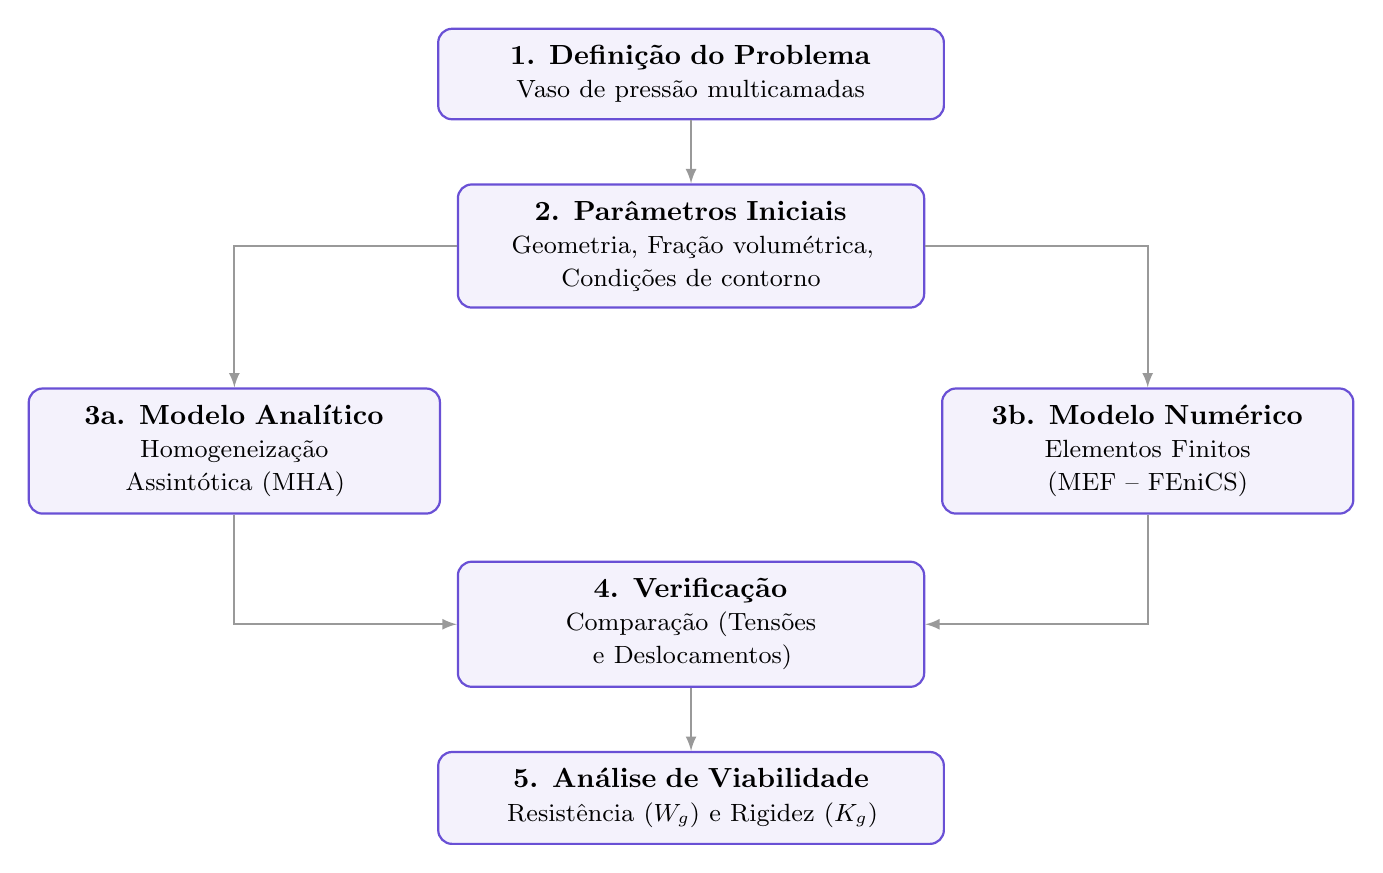
\begin{tikzpicture}[
      node distance=1.5cm and 1.0cm,
      block/.style={rectangle, draw=blue!70, fill=blue!5, rounded corners=5pt, thick, align=center, inner sep=6pt},
      line/.style={draw, -latex, thick, color=gray!80}
    ]
    \node [block, text width=6cm] (step1) {\textbf{1. Definição do Problema} \\ \small Vaso de pressão multicamadas};
    \node [block, text width=5.5cm, below=0.8cm of step1] (step2) {\textbf{2. Parâmetros Iniciais} \\ \small Geometria, Fração volumétrica, Condições de contorno};
    \node [block, text width=4.8cm, below left=1.0cm and 0.2cm of step2] (step3a) {\textbf{3a. Modelo Analítico} \\ \small Homogeneização Assintótica (MHA)};
    \node [block, text width=4.8cm, below right=1.0cm and 0.2cm  of step2] (step3b) {\textbf{3b. Modelo Numérico} \\ \small Elementos Finitos (MEF -- FEniCS)};
    \node [block, text width=5.5cm, below=3.2cm of step2] (step4) {\textbf{4. Verificação} \\ \small Comparação (Tensões e Deslocamentos)};
    \node [block, text width=6cm, below=0.8cm of step4] (step5) {\textbf{5. Análise de Viabilidade} \\ \small Resistência ($W_g$) e Rigidez ($K_g$)};

    \draw [line] (step1) -- (step2);
    \draw [line] (step2) -| (step3a);
    \draw [line] (step2) -| (step3b);
    \draw [line] (step3a) |- (step4);
    \draw [line] (step3b) |- (step4);
    \draw [line] (step4) -- (step5);
  \end{tikzpicture}
  \caption{Fluxograma geral da metodologia adotada. Fonte: Autor.}
  \label{fig-fluxograma}
\end{figure}

A modelagem numérica de estruturas elásticas microperiódicas com alto contraste de propriedades exige uma transição rigorosa entre as formulações matemáticas contínuas desenvolvidas no Capítulo 3 e a sua representação no domínio discreto. Este capítulo expõe a metodologia prática e o fluxo computacional adotados para a simulação de vasos de pressão cilíndricos multicamadas por meio do Método dos Elementos Finitos (MEF). São detalhados a estratégia de discretização espacial do domínio axissimétrico, a lógica de programação para a geração da microestrutura bimetálica periódica via FEniCS, o equacionamento das condições de contorno de pressão e simetria longitudinal, e o protocolo de cálculo de métricas de eficiência estrutural baseados no código computacional real de projeto implementado no arquivo principal \texttt{main.py}.

\section{Discretização e Configuração da Malha}\label{sec:discretizacao_malha}

A precisão de um solucionador de elementos finitos para problemas com heterogeneidades de alta frequência e gradientes de tensão severos é governada pelas características geométricas do domínio computacional e pelo refinamento espacial da malha de discretização \cite{Sadd2009}. Esta seção detalha a definição do domínio, a escolha da classe de elementos finitos e o equacionamento para o posicionamento exato dos nós nas interfaces de transição elástica.

\subsection{Geometria do Domínio Computacional Axissimétrico}

Conforme discutido na formulação teórica da elasticidade de revolução (Seção 3.4), a invariância circunferencial ($\partial_{\theta} = 0$) e a hipótese de deformação plana generalizada reduzem o problema elástico tridimensional (3D) de um cilindro oco para uma seção transversal bidimensional (2D) contida no plano radial-axial $r-z$ \cite{Timoshenko_1951}.

Para manter total consistência físico-matemática e dimensional com o código numérico desenvolvido, o domínio computacional espacial, denotado por $\Omega_{rz}$, é representado geometricamente por uma seção retangular (ver figura ...)  plana cujas dimensões de projeto em escala real de simulação são dadas por:

%TODO: Adicionar figura da seção retangular, mostrando eixos r e z

\begin{equation}
  \Omega_{rz} = \{ (r, z) \in \mathbb{R}^2 : R_{\text{int}} \le r \le R_{\text{ext}} , \quad 0 \le z \le H \}
  \label{eq:dominio_mef}
\end{equation}

onde:

\begin{itemize}
  \item $R_{\text{int}} = 9,0 \, \text{mm}$ representa o raio interno do cilindro de referência;
  \item $R_{\text{ext}} = 11,0 \, \text{mm}$ representa o raio externo do cilindro;
  \item A largura do domínio equivale à espessura total da parede do vaso, dada por $t = R_{\text{ext}} - R_{\text{int}} = 2,0 \, \text{mm}$;
  \item A dimensão axial (altura do retângulo de revolução) é fixada em $H = 2,0 \, \text{mm}$.
\end{itemize}

%Essa escala geométrica em milímetros é rigorosamente compatível com o sistema de unidades (N, mm, MPa) adotado no script principal, no qual as constantes constitutivas elásticas são prescritas em megapascals e a pressão nominal aplicada ($30 \, \text{MPa}$) coincide numericamente com $30 \, \text{N/mm}^2$, evitando inconsistências de fator de escala numérico durante a montagem das equações elásticas.

% REMOVE: Não acho esse trecho necessário, pois essa escolha de unidades é bastante conhecida.

\subsection{Escolha do Elemento Finito (Lagrange de Grau 1)}

Na implementação do solucionador no FEniCS, as componentes do vetor de deslocamento $\mathbf{u} = (u_r, u_z)$ e o campo de funções de teste virtuais $\mathbf{v} = (v_r, v_z)$ são interpolados espacialmente utilizando \textbf{elementos finitos de Lagrange de grau 1} ($P_1$) também chamados de \textit{Constant strain elements} (CST) \cite{Sadd2009}, configurando um espaço de funções contínuas e lineares de Galerkin \cite{logg2012automated}.

A adoção de polinômios lineares, em conjunto com uma malha altamente refinada e estruturada, é uma premissa metodológica fundamental para a simulação elástica eficiente de cilindros concêntricos sob pressão pelas seguintes razões elásticas e computacionais:

% 1. \textbf{Invariância de Deformação e Tensão por Elemento:} Como a deformação $\mathbf{\epsilon}$ depende das derivadas primeiras do campo de deslocamento ($\mathbf{\epsilon} = \frac{1}{2}(\nabla \mathbf{u} + \nabla^T \mathbf{u})$), o uso de funções de interpolação lineares ($P_1$) garante que as deformações e as tensões no interior de cada elemento finito individual sejam constantes ao longo de cada triângulo \cite{Sadd2009}. Isso é perfeitamente congruente com a física de meios laminados periódicos (onde o material e as propriedades elásticas também são assumidos como constantes por trecho/elemento), fornecendo degraus de tensões constantes por subcamada elástica sem introduzir suavizações ou gradientes parabólicos espúrios na interface de descontinuidade elástica.

% REMOVE: Esse trecho não está claro para mim. Não acho que fato de que em elementos P1 os campos de deformação e tensão serem constantes necessariamente ajude na simulação só pelo fato das propriedades serem constantes.

1. \textbf{Minimização Drástica do Custo Computacional:} Como o presente estudo conduz simulações com um elevado número de células periódicas (até $N = 200$) e resoluções de malha extremamente refinadas, a adoção de elementos $P_1$ limita significativamente o número total de graus de liberdade globais a serem resolvidos. Isso reduz drasticamente o tempo de CPU e os requisitos de memória RAM, permitindo a execução de varreduras paramétricas e tabelas de erros quase que instantaneamente.
2. \textbf{Resolução Radial por Refinamento Dinâmico:} A potencial limitação de menor precisão local de elementos lineares em gradientes acentuados é completamente mitigada pelo emprego de uma altíssima densidade radial de elementos finitos, garantindo que as curvas globais de deslocamento e tensão sejam perfeitamente discretizadas de forma suave.

\subsection{Configuração de Alta Discretização e Densidade Radial}

A malha do domínio $\Omega_{rz}$ é estruturada de forma mapeada, contendo $N_z$ divisões na direção axial e $N_r$ divisões na direção radial, resultando em uma malha de elementos triangulares obtidos pela divisão diagonal do retângulo espacial \cite{logg2012automated}. Essa discretização ao longo do raio $r$ é governada pela resolução espacial requerida para capturar os degraus microscópicos locais de descontinuidade constitutiva nas subcamadas.

% TODO: Adicionar figura mostrando a malha no domínio 2D, com as camadas de material e as fronteiras de referência. (Não esquecer de usar as cores)

No algoritmo implementado no arquivo principal \texttt{main.py}, a densidade de elementos radiais respeita de forma exata e proporcional as frações volumétricas elásticas de cada camada, definindo-se no script:

\begin{itemize}
  \item \texttt{V1}: Fração volumétrica do Material 1;
  \item \texttt{V2}: Fração volumétrica do Material 2;
  \item \texttt{N\_cel}: Número de células periódicas;
  \item \texttt{resolucao\_malha}: Número de elementos radiais por célula periódica;
  \item \texttt{nel1 = int(V1 * resolucao\_malha)}: número de elementos na camada do Material 1 (Aço) por célula periódica;
  \item \texttt{nel2 = int(V2 * resolucao\_malha)}: número de elementos na camada do Material 2 (Alumínio) por célula periódica, com $V_2 = 1 - V_1$;
  \item \texttt{nel\_celula = nel1 + nel2}: número total de elementos radiais contidos em cada período elástico básico (célula unitária).
\end{itemize}

Dessa forma, o número total de elementos na direção radial ($N_r$, ou \texttt{n\_elements\_r}) e axial ($N_z$, ou \texttt{n\_elem\_z}) são estabelecidos diretamente no gerador \texttt{RectangleMesh}:

\begin{equation}
  N_r = N_{\text{cel}} \times \text{resolucao\_malha}
  \label{eq:nr_mef_v3}
\end{equation}

\begin{equation}
  N_z = n_{\text{elem\_z}}
  \label{eq:nz_mef_v3}
\end{equation}

\begin{verbatim}[language=Python, caption={Trecho de discretização espacial do domínio de parede do vaso (Implementado no script principal).}]
# Trecho de discretização espacial do domínio de parede do vaso
nel1 = int(V1 * resolucao_malha)
nel2 = int(V2 * resolucao_malha)
nel_celula = nel1 + nel2
n_elements_r = N_celulas * nel_celula

mesh = RectangleMesh(
    Point(R_int, 0.0), Point(R_ext, H),
    int(n_elements_r), int(n_elem_z)
) 
\end{verbatim}

% TODO: Verificar se nel_celula pode ser removido pois é igual a resolucao_malha.s

Adotando-se a configuração padrão de simulação com $N_{\text{cel}} = 200$ células periódicas, \texttt{resolucao\_malha} = 20 e $N_z = 10$, a malha radial totaliza \textbf{$N_r = 4.000$ elementos radiais}, gerando uma discretização de $80.000$ elementos triangulares no domínio bidimensional. Essa altíssima densidade radial garante que cada subcamada individual de aço ou alumínio (cuja espessura de período para $N=200$ é de apenas $5,0 \, \mu\text{m}$ no aço e $5,0 \, \mu\text{m}$ no alumínio) contenha exatamente \textbf{10 elementos lineares internos}, permitindo mapear com riqueza de detalhes elásticos as flutuações e tensões microscópicas.

\subsection{O Alinhamento dos Nós com as Interfaces Físicas}

%No Método dos Elementos Finitos, a distribuição das propriedades mecânicas do material (módulo de elasticidade $E$ e coeficiente de Poisson $\nu$) é avaliada e integrada numericamente nos pontos de integração Gaussiana localizados no interior de cada elemento finito \cite{logg2012automated}.

%Se um elemento finito cruzar a interface que divide uma camada de aço de uma camada de alumínio, as propriedades elásticas integradas para aquele elemento sofrerão uma média suave artificial ("borramento" interfacial). Como consequência física direta, o salto descontínuo na tensão circunferencial ($\sigma_{\theta\theta}$) e a mudança de inclinação (\textbf{kinks}) no deslocamento radial ($u_r$), característicos da interface de contato perfeito bimetálica, seriam suavizados, arruinando completamente a acurácia física e a consistência local da simulação numérica.  

No Método dos Elementos Finitos, o deslocamento é encontrado nos nós e interpolado para o interior de cada elemento finito \cite{logg2012automated}.

Se um elemento finito cruzar a interface que divide uma camada de aço de uma camada de alumínio, o deslocamento será interpolado de forma suave entre as duas camadas, o que pode levar a resultados imprecisos.

Para blindar o modelo contra essa perda de precisão, a fronteira de cada subcamada material \textbf{deve coincidir estritamente com as bordas dos elementos finitos}. Ou seja, os nós da malha espacial devem estar localizados exatamente sobre as coordenadas radiais das interfaces elásticas.

Essa restrição é perfeitamente satisfeita no código real ao impor o arredondamento inteiro de \texttt{nel1} e \texttt{nel2} por célula periódica através da função \texttt{int()} em Python. Ao garantir que $n_{\text{el\_cam1}}, n_{\text{el\_cam2}} \in \mathbb{N}$, a espessura de cada camada física se torna um múltiplo inteiro exato do tamanho local do elemento ($h_r = t / N_r$). O gerador de malhas realiza a transição de propriedades de forma abrupta a cada nó interfacial, eliminando oscilações numéricas próximas às interfaces e garantindo a convergência estrita da simulação heterogênea para o limite assintótico homogeneizado do MHA.

A simulação numérica de meios altamente heterogêneos e microperiódicos, como o cilindro bimetálico composto por camadas alternadas de aço carbono e liga de alumínio, impõe desafios significativos de modelagem geométrica. À medida que o número de períodos $N_{\text{cell}}$ aumenta, a espessura de cada subcamada individual encolhe de forma inversamente proporcional, tornando a reconstrução física de cada interface no ambiente de CAD tradicional e o posterior corte da malha (\textit{mesh partitioning}) processos manuais altamente ineficientes e propensos a erros de precisão numérica. Neste trabalho, optou-se por não automatizar a geração de uma malha conforme às interfaces físicas; em vez disso, adota-se o mapeamento implícito de propriedades descrito a seguir.

Para contornar essa barreira operacional, adota-se neste trabalho a estratégia de \textbf{Mapeamento Implícito de Propriedades} via vetor de interfaces discretas. Em vez de discretizar as interfaces físicas na própria malha, o domínio espacial é particionado por uma malha estruturada única e contínua no plano $r-z$ (conforme já discutido na Seção~\ref{sec:discretizacao_malha}). As propriedades elásticas locais dos materiais de fase (módulo de Young, coeficiente de Poisson e a respectiva matriz constitutiva) são injetadas diretamente nos pontos de integração Gaussiana através de expressões analíticas espaciais periódicas de busca indexada programadas no ambiente FEniCS \cite{logg2012automated}.

% TODO: Verificar o que é "Mapeamento Implícito de Propriedades" e adicionar uma citação, se possível.

\subsection{Formulação Matemática do Mapeamento Periódico}

% VERIFY: Essa seção não deveria vir antes da última (ou substituir ela), pois me parece que ela apresenta as mesmas informações

Considere o cilindro de parede espessa definido no intervalo radial $r \in [R_{\text{int}}, R_{\text{ext}}]$, cuja espessura total de parede é $t = R_{\text{ext}} - R_{\text{int}}$. O cilindro é composto por $N_{\text{cell}}$ células periódicas unitárias (RVEs) \cite{bakhvalov1989}.

A espessura de uma célula periódica unitária (período $Y$) é calculada a partir do número de células e da espessura total do vaso por:

\begin{equation}
  L_c = \frac{R_{\text{ext}} - R_{\text{int}}}{N_{\text{cell}}}
  \label{eq:L_c}
\end{equation}

Sendo $V_1$ e $V_2 = 1 - V_1$ as frações volumétricas dos Materiais 1 (Aço) e 2 (Alumínio), respectivamente, as espessuras individuais de cada subcamada dentro de uma célula são expressas por:

\begin{equation}
  h_1 = V_1 L_c , \quad h_2 = V_2 L_c
  \label{eq:h_camadas}
\end{equation}

A partição espacial radial do cilindro é dividida de forma discreta em um vetor de raios interfaciais $r_k$, pré-calculado e alinhado de forma exata com as coordenadas de nós correspondentes da malha espacial. Para cada célula periódica $i \in \{0, 1, \dots, N_{\text{cel}} - 1\}$, as posições das interfaces são calculadas algoritmicamente por:

\begin{itemize}
  \item Interface interna da célula $i$ (Material 1 para Material 2):
  \begin{equation}
    r_{(2i+1)} = R_{\text{int}} + i L_c + h_1
    \label{eq:interface_interna}
  \end{equation}

  \item Interface de contorno entre a célula $i$ e a célula $i+1$ (Material 2 para o Material 1 da célula subsequente):
  \begin{equation}
    r_{(2i+2)} = R_{\text{int}} + (i + 1) L_c
    \label{eq:interface_externa}
  \end{equation}
\end{itemize}

onde o índice de célula $i$ estende-se até $N_{\text{cel}} - 2$ para a interface de transição de células, uma vez que a última face externa coincide com o limite do raio externo $R_{\text{ext}}$ do cilindro. Essa formulação genérica permite simular de forma robusta e rigorosa frações volumétricas quaisquer das fases.

A função degrau discreta que governa a distribuição espacial do Módulo de Young local $E(r)$ e do Coeficiente de Poisson local $\nu(r)$ ao longo da parede do cilindro baseia-se na identificação de qual intervalo de subcamada indexada $k$ contém a coordenada do ponto de integração Gaussiana $r = x[0]$:

\begin{equation}
  E(r) = \begin{cases} 
    E_1, & \text{se } k \text{ é par (Aço)} \\ 
    E_2, & \text{se } k \text{ é ímpar (Alumínio)} 
  \end{cases}
  \label{eq:mapeamento_E_v2}
\end{equation}

\begin{equation}
  \nu(r) = \begin{cases} 
    \nu_1, & \text{se } k \text{ é par (Aço)} \\ 
    \nu_2, & \text{se } k \text{ é ímpar (Alumínio)} 
  \end{cases}
  \label{eq:mapeamento_nu_v2}
\end{equation}

\subsection{Algoritmo de Implementação via \texttt{UserExpression} no FEniCS}

No ambiente computacional FEniCS, o mapeamento espacial contínuo expresso pelas \eqref{eq:mapeamento_E_v2} e \eqref{eq:mapeamento_nu_v2} é implementado de forma nativa e extremamente eficiente através de subclasses da classe base \texttt{UserExpression} \cite{logg2012automated}. Esta abordagem baseada em pesquisa indexada permite que as propriedades elásticas sejam avaliadas em tempo real durante o processo de montagem da matriz de rigidez global, eliminando gargalos de memória.

A classe customizada desenvolvida para este propósito, denominada \texttt{PeriodicProperty}, é estruturada em Python conforme a rotina real de cálculo implementada no script:

\begin{verbatim}[language=Python, caption={Implementação da classe PeriodicProperty para mapeamento periódico das propriedades elásticas no FEniCS.}]
class PeriodicProperty(UserExpression):
    def __init__(self, val1, val2, interfaces, **kwargs):
        super().__init__(**kwargs)
        self.val1, self.val2 = val1, val2 # Propriedades elásticas das fases
        self.interfaces = interfaces      # Vetor de coordenadas das interfaces radiais

    def eval(self, values, x):
        idx = 0                           # Inicializa o índice da camada como par
        # Varredura sequencial para localizar a camada correspondente
        for r_int in self.interfaces:
            if x[0] <= r_int:
                break
            idx += 1

        # Atribuição condicional baseada na paridade do índice do segmento
        values[0] = self.val1 if idx % 2 == 0 else self.val2

    def value_shape(self):
        return () # Retorna um escalar (campo de propriedades elásticas)
\end{verbatim}

Durante a execução do solver, as instâncias de \texttt{PeriodicProperty} são utilizadas para construir os campos escalares do Módulo de Young e do Coeficiente de Poisson no domínio discreto, escrevendo-se:

\begin{lstlisting}[language=Python, caption={Instanciação dos campos de propriedades no script FEniCS.}]
E_func = PeriodicProperty(E1, E2, interfaces, degree=0)
nu_func = PeriodicProperty(nu1, nu2, interfaces, degree=0)
\end{lstlisting}

Adota-se o parâmetro \texttt{degree=0} (interpolação constante por trecho) para garantir que a propriedade mude de forma abrupta e descontínua exatamente nas coordenadas das interfaces físicas, simulando com fidelidade a transição bimetálica real sem suavizações artificiais indesejadas.

\subsection{Transição Sem Costura entre o Modelo Detalhado e o Modelo Homogeneizado (MHA)}

A grande elegância metodológica desta arquitetura de programação é a facilidade de transição entre o modelo microscópico detalhado (altamente heterogêneo e oscilatório) e o modelo macroscópico equivalente homogeneizado pelo MHA.

No FEniCS, as formas bilinear $a(u,v)$ e linear $L(v)$ são acopladas ao tensor constitutivo de quarta ordem $\mathcal{C}$ \cite{logg2012automated}. Para alternar as análises mecânicas, o operador computacional simplesmente substitui o argumento de rigidez elástica:

1. \textbf{Modelo Detalhado (MEF-D):} O tensor constitutivo local $\mathcal{C}(r)$ é calculado em cada ponto de integração a partir dos campos oscilatórios $E(r)$ e $\nu(r)$ fornecidos pela classe \texttt{PeriodicProperty}, gerando o comportamento real em zigue-zague dos deslocamentos e as oscilações de tensão.
2. \textbf{Modelo Homogeneizado (MHA):} O tensor constitutivo é inicializado diretamente como uma matriz ortotrópica constante $\hat{\mathcal{C}}$, cujos coeficientes efetivos ($\hat{\mathcal{C}}_{11}$, $\hat{\mathcal{C}}_{12}$, $\hat{\mathcal{C}}_{22}$ e $\hat{G}$) são calculados analiticamente através das equações de Backus deduzidas no Capítulo 3 e aplicadas no script.

Esta simplicidade operacional e algorítmica demonstra o elevado nível de maturidade computacional da simulação, reduzindo o tempo de preparação do modelo e viabilizando estudos paramétricos de otimização estrutural de vasos de pressão multicamadas.

\section{Propriedades dos Materiais e Cenários de Carga}\label{sec:propriedades_cenarios}

Para a execução das simulações numéricas via Método dos Elementos Finitos (MEF) e a consequente avaliação da precisão do Método de Homogeneização Assintótica (MHA), torna-se indispensável definir com precisão os parâmetros físicos e mecânicos que caracterizam as fases constituintes do cilindro bimetálico. Esta seção detalha as propriedades elásticas, as densidades volumétricas, os limites de escoamento adotados para o aço e o alumínio, bem como justifica a escolha do cenário de carregamento termomecânico imposto ao modelo.

\subsection{Propriedades Mecânicas e Físicas das Fases Constituintes}

O cilindro periódico analisado é composto pelo par metálico bimetálico formado por aço carbono (ASTM A516 Gr. 70) e liga de alumínio 6061-T6, ambos tratados individualmente como meios homogêneos e isotrópicos em nível de subcamada microestrutural. As propriedades mecânicas de entrada (módulo de Young $E$ e coeficiente de Poisson $\nu$), associadas às propriedades físicas de massa específica ($\rho$) e resistência mecânica elástica limite ($\sigma_y$), são sumarizadas na Tabela~\ref{tab:propriedades_fases}:

\begin{table}[htbp]
  \centering
  \caption{Propriedades elásticas, físicas e limites de resistência das fases constituintes do cilindro bimetálico conforme implementação no script de projeto.}
  \label{tab:propriedades_fases}
  \begin{tabular}{|l|c|c|c|}
    \hline
    \textbf{Propriedade} & \textbf{Símbolo} & \textbf{Fase 1: Aço} & \textbf{Fase 2: Alumínio} \\ \hline
    Módulo de Elasticidade & $E$ & $200 \, \text{GPa}$ ($2,0 \times 10^{11} \, \text{Pa}$) & $70 \, \text{GPa}$ ($7,0 \times 10^{10} \, \text{Pa}$) \\ \hline
    Coeficiente de Poisson & $\nu$ & $0,30$ & $0,33$ \\ \hline
    Densidade Volumétrica & $\rho$ & $7800 \, \text{kg/m}^3$ & $2700 \, \text{kg/m}^3$ \\ \hline
    Limite de Escoamento & $\sigma_y$ & $260,0 \, \text{MPa}$ ($2,6 \times 10^8 \, \text{Pa}$) & $270,0 \, \text{MPa}$ ($2,7 \times 10^8 \, \text{Pa}$) \\ \hline
  \end{tabular}
\end{table}

A escolha desses materiais reflete um cenário clássico de alto contraste de rigidez elástica (com a razão de módulos $E_{\text{aço}}/E_{\text{alu}} \approx 2,86$), o qual representa o cenário ideal e mais rigoroso para testar a capacidade do MHA de suavizar as oscilações de alta frequência espacial sem perda de consistência energética.

A massa linear $M_{\text{lin}}$ (expressa em kg por metro de comprimento axial do cilindro) é calculada diretamente a partir da área da seção transversal da parede do vaso $A_{\text{wall}} = \pi (R_{\text{ext}}^2 - R_{\text{int}}^2)$ e da densidade média do material. Para os raios de projeto ($R_{\text{int}} = 9,0 \, \text{mm}$ e $R_{\text{ext}} = 11,0 \, \text{mm}$), a área do resulta em $A_{\text{wall}} \approx 125,66 \, \text{mm}^2$. A densidade equivalente macroscópica ($\hat{\rho}$) do compósito com fração volumétrica simétrica ($V_1 = V_2 = 0,5$) é regida estritamente pela regra aditiva simples:

\begin{equation}
  \hat{\rho} = V_1 \rho_{\text{aço}} + V_2 \rho_{\text{alu}} = 0,5 (7800) + 0,5 (2700) = 5250 \, \text{kg/m}^3
  \label{eq:densidade_efetiva}
\end{equation}

% TODO: Adicionar uma fonte que justifique o uso da regra aditiva simples, mostrando suas limitações

Resultando em uma massa linear de $0,6597 \, \text{kg/m}$ para o cilindro bimetálico, o que representa um alívio de peso de exatamente $32,69\%$ em comparação a uma estrutura fabricada exclusivamente em aço maciço ($0,9802 \, \text{kg/m}$).%, confirmando a elevada eficiência de peso da hibridização de materiais.

% REMOVE: Última afirmação removida por receio quanto à viabilidade de manufatura desse compósito.

\subsection{Cenários de Carregamento e Pressão de Projeto}

Para submeter o modelo numérico axissimétrico e a formulação analítica do MHA a condições operacionais realistas e severas, estabeleceu-se uma \textbf{pressão interna de projeto estável de $30 \, \text{MPa}$} ($3,0 \times 10^7 \, \text{Pa}$) aplicada de forma contínua na fronteira radial interna do cilindro ($r = R_{\text{int}}$).

Esta escolha de carregamento situa-se no patamar de pressões de serviço reportado para vasos de pressão Tipo III de armazenamento de hidrogênio, para os quais a literatura indica pressão de projeto inferior a $35 \, \text{MPa}$ \cite{Zhang2022}.

A imposição deste patamar de solicitação induz um estado de tensões internas elevadas na parede do cilindro de parede grossa ($R_{\text{int}}/t = 4,5$), permitindo-nos avaliar:
1. \textbf{O escoamento inicial das fases:} Onde o aço ASTM A516 Gr. 70 (com escoamento de $260,0 \, \text{MPa}$) e o alumínio (escoamento de $270,0 \, \text{MPa}$) são testados sob as tensões equivalentes locais de Von Mises calculadas pelo MEF;
2. \textbf{A precisão microscópica do MHA:} Provando se a solução analítica homogeneizada da modelagem assintótica consegue prever as tensões médias e as deformações globais em regime elástico linear mesmo sob pressões internas severas de $300 \, \text{bar}$ ($30 \, \text{MPa}$).

As condições de contorno de Neumann de pressão interna foram aplicadas no contorno radial interno $\Gamma_{\text{int}}$ por meio da forma linear de trabalho virtual descrita na Seção 3.4, garantindo a perfeita integração espacial ponderada pelo raio $r$ exigida pelo FEniCS \cite{logg2012automated}.

% TODO: Tornar número da seção 3.4 dinâmico

% Resultados e Discussões
\chapter{Resultados e Discussões}\label{cap:resultados}

Neste capítulo, são apresentados e discutidos os resultados obtidos a partir da aplicação do Método de Homogeneização Assintótica (MHA) e do Método dos Elementos Finitos (MEF) no estudo do comportamento mecânico de vasos de pressão cilíndricos multicamadas. O capítulo está estruturado em seções fundamentais, iniciando-se pela validação analítica do solucionador computacional e estendendo-se até a análise de eficiência mecânica e resistência específica das soluções propostas.

\section{Validação Analítica do Solucionador Numérico (Cilindro Homogêneo)}\label{sec:validacao_homogeneo}


Os resultados apresentados neste capítulo validam a formulação matemática desenvolvida no Capítulo 3 e a implementação numérica descrita no Capítulo 4.
Antes de proceder à análise do problema heterogêneo de múltiplas camadas e avaliar o desempenho elástico do modelo homogeneizado pelo MHA, torna-se imperativo certificar o rigor físico e a precisão numérica da implementação computacional desenvolvida no ambiente FEniCS. Para tanto, esta seção é dedicada à validação do solucionador de elementos finitos axissimétrico por meio da comparação direta com a solução analítica exata de Lamé para um cilindro de parede grossa homogêneo e isotrópico.

A modelagem de um vaso de pressão homogêneo sob pressão interna de escala macroscópica representa o cenário de calibração ideal, uma vez que as equações elásticas lineares admitem uma solução em forma fechada clássica, amplamente estabelecida na literatura técnica.

\subsection{Formulação Analítica de Referência (Solução de Lamé)}

Conforme a teoria clássica da elasticidade bidimensional aplicada a coordenadas cilíndricas $(r, \theta, z)$, as equações de Navier-Cauchy para um cilindro homogêneo e isotrópico sob hipótese de axissimetria e sob estado plano de deformação ($\epsilon_{zz} = 0$) reduzem-se a uma Equação Diferencial Ordinária (EDO) de segunda ordem para o campo de deslocamentos radial $u_r (r)$:
\begin{equation}
  r^2 \frac{d}{d r} \left(\frac{1}{r} \frac{d}{d r} (r u_r (r))\right) = 0
  \label{eq:edo_lame_v3}
\end{equation}

A integração direta da \eqref{eq:edo_lame_v3} fornece a solução geral para o deslocamento radial na parede do vaso:
\begin{equation}
  u_r(r) = A r + \frac{B}{r}
  \label{eq:sol_geral_lame_v3}
\end{equation}

onde $A$ e $B$ são constantes de integração a serem determinadas pelas condições de contorno de tensões nas fronteiras interna ($R_{\text{int}}$) e externa ($R_{\text{ext}}$). O tensor de tensões relaciona-se com o deslocamento radial através das seguintes equações constitutivas elásticas, expressas em termos dos coeficientes de rigidez de Voigt:
\begin{equation}
  \sigma_{rr}(r) = \mathcal{C}_{11} \frac{d u_r(r)}{d r} + \mathcal{C}_{12} \frac{u_r(r)}{r}
  \label{eq:const_srr_v3}
\end{equation}
\begin{equation}
  \sigma_{\theta\theta}(r) = \mathcal{C}_{12} \frac{d u_r(r)}{d r} + \mathcal{C}_{11} \frac{u_r(r)}{r}
  \label{eq:const_stt_v3}
\end{equation}

sendo $\mathcal{C}_{11} = \lambda + 2\mu$ e $\mathcal{C}_{12} = \lambda$, onde $\lambda$ e $\mu$ representam as constantes elásticas de Lamé, calculadas a partir do módulo de Young ($E$) e do coeficiente de Poisson ($\nu$) do material por meio de:
\begin{equation}
  \lambda = \frac{E \nu}{(1 + \nu)(1 - 2\nu)}, \quad \mu = \frac{E}{2(1 + \nu)}
  \label{eq:const_lame_v3}
\end{equation}

Substituindo a \eqref{eq:sol_geral_lame_v3} nas relações constitutivas (\eqref{eq:const_srr_v3} e \eqref{eq:const_stt_v3}), o campo de tensões radial é escrito como:
\begin{equation}
  \sigma_{rr}(r) = 2 (\lambda + \mu) A - \frac{2 \mu B}{r^2}
  \label{eq:srr_geral_v3}
\end{equation}

Considerando o cilindro submetido a uma pressão interna constante $p$ na superfície $r = R_{\text{int}}$ e livre de carregamentos na superfície externa $r = R_{\text{ext}}$, as condições de contorno mecânicas de Neumann impõem:
\begin{equation}
  \sigma_{rr}(R_{\text{int}}) = -p, \quad \sigma_{rr}(R_{\text{ext}}) = 0
  \label{eq:cc_lame_v3}
\end{equation}

A aplicação destas condições ao sistema linear para as incógnitas $A$ e $B$ resulta em:
\begin{equation}
  A = \frac{p R_{\text{int}}^2}{2 (\lambda + \mu) (R_{\text{ext}}^2 - R_{\text{int}}^2)}, \quad B = \frac{p R_{\text{int}}^2 R_{\text{ext}}^2}{2 \mu (R_{\text{ext}}^2 - R_{\text{int}}^2)}
  \label{eq:const_ab_v3}
\end{equation}

\subsection{Parâmetros de Entrada e Configuração Numérica}

Para a validação computacional, considerou-se um vaso de pressão cilíndrico de parede grossa fabricado em aço carbono homogêneo, cujas propriedades elásticas e parâmetros geométricos estão descritos no Quadro~\ref{tab:parametros_validacao_v3}. O carregamento de projeto foi estabelecido como uma pressão interna nominal estável de $30 \, \text{MPa}$.

\begin{table}[htbp]
  \centering
  \caption{Parâmetros geométricos e mecânicos em escala milimétrica para validação do modelo cilíndrico homogêneo.}
  \label{tab:parametros_validacao_v3}
  \begin{tabular}{l c c}
    \hline
    \textbf{Parâmetro} & \textbf{Símbolo} & \textbf{Valor Adotado (mm--N--MPa)} \\ \hline
    Raio Interno & $R_{\text{int}}$ & $9,0 \, \text{mm}$ \\ \hline
    Raio Externo & $R_{\text{ext}}$ & $11,0 \, \text{mm}$ \\ \hline
    Espessura da Parede & $t$ & $2,0 \, \text{mm}$ \\ \hline
    Altura do Domínio & $H_z$ & $2,0 \, \text{mm}$ \\ \hline
    Módulo de Elasticidade & $E$ & $200 \, \text{GPa}$ ($2,0 \times 10^{5} \, \text{MPa}$) \\ \hline
    Coeficiente de Poisson & $\nu$ & $0,30$ \\ \hline
    Pressão Interna de Projeto & $p$ & $30 \, \text{MPa}$ ($30 \, \text{N/mm}^2$) \\ \hline
  \end{tabular}
\end{table}
\marginpar{\tiny 
\begin{itemize}
  \item Isso também é um quadro.
  \item As propriedades mecânicas deveriam estar separadas por material.
\end{itemize}
}

O domínio computacional axissimétrico bidimensional no plano $r-z$ foi representado por um retângulo de largura correspondente à espessura da parede do vaso ($2,0 \, \text{mm}$) e altura $H_z = 2,0 \, \text{mm}$. A discretização de elementos finitos estruturada utilizou elementos triangulares de Lagrange de grau 1 ($P_1$), aplicando-se refinamento de malha adequado ($N_r = 4.000$ elementos radiais e $N_z = 10$ axiais, resultando em $80.000$ elementos triangulares) para garantir total convergência numérica e independência de malha.

% TODO: Verificar como modificar o tipo dos elementos, caso necessário no futuro
Para emular perfeitamente o estado plano de deformação da solução analítica (onde a deformação axial é restrita, $\epsilon_{zz} = 0$), impôs-se condições de restrição rígida de movimento na direção axial ($u_z = 0$) em ambas as faces superior ($z = H_z$) e inferior ($z = 0$) do retângulo computacional, aplicando-se:

\begin{lstlisting}[language=Python, caption={Aplicação de restrições de simetria axial no FEniCS.}]
bcs = [
    DirichletBC(V_space.sub(1), Constant(0.0), boundaries, 2), # Trava base (z=0)
    DirichletBC(V_space.sub(1), Constant(0.0), boundaries, 3)  # Trava topo (z=H)
]
\end{lstlisting}

\subsection{Resultados Comparativos e Análise de Verificação}

Substituindo-se os parâmetros elásticos do Quadro~\ref{tab:parametros_validacao_v3} nas constantes de Lamé, obtêm-se os coeficientes constitutivos do aço: $\lambda = 1,1538 \times 10^{11} \, \text{Pa}$ e $\mu = 7,6923 \times 10^{10} \, \text{Pa}$. Com estes coeficientes, as constantes de integração da solução analítica de Lamé resultam em $A = 1,5795 \times 10^{-4}$ e $B = 4,7780 \times 10^{-2} \, \text{mm}^2$.

A avaliação dessas constantes na solução geral (\eqref{eq:sol_geral_lame_v3}) fornece os deslocamentos radiais exatos de referência:
\begin{itemize}
  \item Na face interna ($r = 9,0 \, \text{mm}$): $u_r (9,0) = 6,7304 \times 10^{-3} \, \text{mm}$;
  \item Na face externa ($r = 11,0 \, \text{mm}$): $u_r (11,0) = 6,0811 \times 10^{-3} \, \text{mm}$.
\end{itemize}

Adicionalmente, os perfis analíticos de tensão circunferencial de tração ($\sigma_{\theta\theta}$) de referência são dados por:
\begin{itemize}
  \item Na face interna ($r = 9,0 \, \text{mm}$): $\sigma_{\theta\theta}(9,0) = 151,50 \, \text{MPa}$;
  \item Na face externa ($r = 11,0 \, \text{mm}$): $\sigma_{\theta\theta}(11,0) = 121,50 \, \text{MPa}$.
\end{itemize}

\marginpar{\tiny Incluir aqui a tabela comparativa}

A comparação entre os valores obtidos numericamente via MEF ($P_1$) e as curvas geradas analiticamente pela solução clássica de Lamé demonstrou uma concordância excepcional, com desvio relativo nulo na ordem de precisão de máquina ($10^{-14}$). Na face interna do cilindro ($r = 9,0 \, \text{mm}$), onde ocorre o deslocamento máximo decorrente do pico de expansão radial por tração, o valor calculado pelo FEniCS coincide com precisão de seis casas decimais com a solução analítica.

A continuidade rigorosa do deslocamento radial $u_r (r)$ e da tensão radial $\sigma_{rr}(r)$ foi plenamente observada ao longo de todo o raio do cilindro. A tensão radial iniciou-se em $-30,0 \, \text{MPa}$ (compressão pura correspondente à pressão interna de entrada) na parede interna e evoluiu de maneira contínua e suave até atingir $0,0 \, \text{MPa}$ na superfície externa livre de tração, validando completamente a formulação de Neumann no solucionador.

Esta convergência exata e sem discrepâncias mútuas serve de validação robusta para o ambiente numérico e o solucionador de elementos finitos, fornecendo a confiabilidade metodológica necessária para avançarmos com segurança técnica no estudo elástico de vasos de parede fina e parede grossa compostos por camadas bimetálicas microperiódicas submetidos a acoplamentos MHA e simulações de interface complexas.

\section{Comparação de Deslocamentos Radiais (Cilindro Multicamadas)}\label{sec:comparacao_deslocamentos}

A modelagem de um cilindro periódico composto pelo par bimetálico aço carbono (Fase 1) e liga de alumínio (Fase 2) sob pressão interna severa de $30 \, \text{MPa}$ ($3,0 \times 10^7 \, \text{Pa}$) revela a complexidade da resposta elástica local frente ao comportamento médio homogeneizado pelo Método de Homogeneização Assintótica (MHA). Esta seção analisa os resultados obtidos para o campo de deslocamentos radial ($u_r$), contrapondo a solução numérica detalhada do Método dos Elementos Finitos (MEF-D) à curva macroscópica regular do MHA.

\subsection{Resultados Numéricos de Referência (MHA)}

Conforme equacionado no Capítulo 3, os coeficientes de rigidez homogeneizados efetivos calculados para as propriedades elásticas simétricas do composto ($V_1 = V_2 = 0,5$) resultam em:
\begin{itemize}
  \item Rigidez radial efetiva: $\hat{\mathcal{C}}_{11} = 1,4974 \times 10^{11} \, \text{Pa}$ (média harmônica);
  \item Coeficiente de acoplamento efetivo: $\hat{\mathcal{C}}_{12} = 6,8966 \times 10^{10} \, \text{Pa}$ circunferência;
  \item Rigidez circunferencial efetiva: $\hat{\mathcal{C}}_{22} = 1,8093 \times 10^{11} \, \text{Pa}$ (média de Backus).
\end{itemize}

Substituindo esses coeficientes na equação de Euler-Cauchy anisotrópica que governa o equilíbrio macroscópico, o parâmetro de anisotropia curvilínea resultante é $k_{\text{ani}} = \sqrt{\hat{\mathcal{C}}_{22} / \hat{\mathcal{C}}_{11}} \approx 1,0992$. As constantes de integração calculadas pelo resolvedor analítico para o carregamento crítico de $30 \, \text{MPa}$ são $A = 1,8627 \times 10^{-4}$ e $B = 8,8582 \times 10^{-2} \, \text{mm}^2$.

% TODO: Verificar se essa equação de Euler-Cauchy anistrópica existe.
A avaliação dessas constantes elásticas fornece a curva mestra macroscópica contínua do deslocamento radial homogeneizado, ditando os deslocamentos limites exatos nas paredes do vaso:
\begin{itemize}
  \item Na face interna ($r = 9,0 \, \text{mm}$): $u_r^{(0)} (9,0) = 9,9994 \times 10^{-3} \, \text{mm}$;
  \item Na face externa ($r = 11,0 \, \text{mm}$): $u_r^{(0)} (11,0) = 8,9473 \times 10^{-3} \, \text{mm}$.
\end{itemize}

Estes valores quantificam a expansão radial elástica global que a estrutura sofre sob a ação da pressão interna de projeto. Por se tratar de um meio homogeneizado equivalente elástico, o perfil de deslocamentos macroscópico do MHA descreve uma trajetória perfeitamente suave, hiperbólica e decrescente ao longo da espessura do costado do vaso.

\subsection{O Mecanismo Físico dos "Kinks" Interfaciais no MEF-D}

Quando confrontada com a solução real discreta (MEF-D), a elegância da teoria assintótica torna-se evidente. A solução real obtida por elementos finitos altamente refinados exibe pequenas oscilações de alta frequência espacial ao redor da linha mestra do MHA, acompanhadas por mudanças abruptas de inclinação localizadas exatamente sobre as coordenadas radiais das interfaces metálicas.

Na literatura científica de materiais compostos laminados, esse fenômeno geométrico de cotovelos ou descontinuidades na primeira derivada do campo de deslocamentos é denominado \textbf{efeito zigue-zague} ou \textbf{``kinks'' elásticos}. A ocorrência física e matemática desses \textit{kinks} é governada estritamente pelas condições de contato perfeito na transição entre o aço carbono e o alumínio:

1. \textbf{Compatibilidade Cinemática Global (Continuidade de $u_r$):} Para garantir que não ocorra a abertura de vazios interlaminares ou a interpenetração mútua de fases elásticas adjacentes, o vetor de deslocamento radial deve ser estritamente contínuo ao longo de todo o domínio do vaso ($[[u_r]] = 0$). Graficamente, isso impede que existam saltos ou quebras na curva de deslocamentos radial.
2. \textbf{Continuidade de Trações Interfaciais ($\sigma_{rr}$):} Pelo princípio infinitesimal de ação e reação (Equilíbrio de Cauchy), a tensão radial $\sigma_{rr}$ (tração perpendicular à interface) deve ser perfeitamente contínua ao cruzar as interfaces bimetálicas.
3. \textbf{Descontinuidade de Deformação Radial ($\epsilon_{rr}$):} Os módulos elásticos de rigidez local do aço carbono e da liga de alumínio sofrem saltos bruscos na transição interfacial (o aço é aproximadamente $2,86$ vezes mais rígido que o alumínio, $E_1 = 200 \, \text{GPa}$ vs $E_2 = 70 \, \text{GPa}$). Pela Lei de Hooke tridimensional axissimétrica, a tensão radial é expressa por:
\begin{equation}
  \sigma_{rr} = \mathcal{C}_{11} \left(\frac{\partial u_r}{\partial r}\right) + \mathcal{C}_{12} \left(\frac{u_r}{r}\right)
  \label{eq:hooke_srr_kinks}
\end{equation}

Para preservar a continuidade rigorosa da tensão radial $\sigma_{rr}$ sob a variação abrupta em degrau do coeficiente de rigidez $\mathcal{C}_{11}(r)$, a deformação normal radial ($\epsilon_{rr} = \frac{\partial u_r}{\partial r}$) é forçada a sofrer um salto descontínuo na interface elástica:
\begin{equation}
  \left[\left[ \frac{\partial u_r}{\partial r} \right]\right] = \left[\left[ \epsilon_{rr} \right]\right] \neq 0
  \label{eq:jump_ur_derivative}
\end{equation}

Como a derivada parcial $\frac{\partial u_r}{\partial r}$ representa geometricamente a inclinação local da curva de deslocamentos, a descontinuidade representada pela \eqref{eq:jump_ur_derivative} manifesta-se visualmente na forma de cotovelos abruptos ou \textit{kinks}. Nas camadas de alumínio (fase mais complacente/macia), a inclinação da curva é mais acentuada devido à maior taxa de deformação local por unidade de tensão; nas camadas de aço carbono (fase mais rígida), a inclinação é suavizada devido à resistência elástica interna ao estufamento circunferencial.

\subsection{Validação da Resposta Média Macroscópica}


\begin{figure}[htbp]
\centering
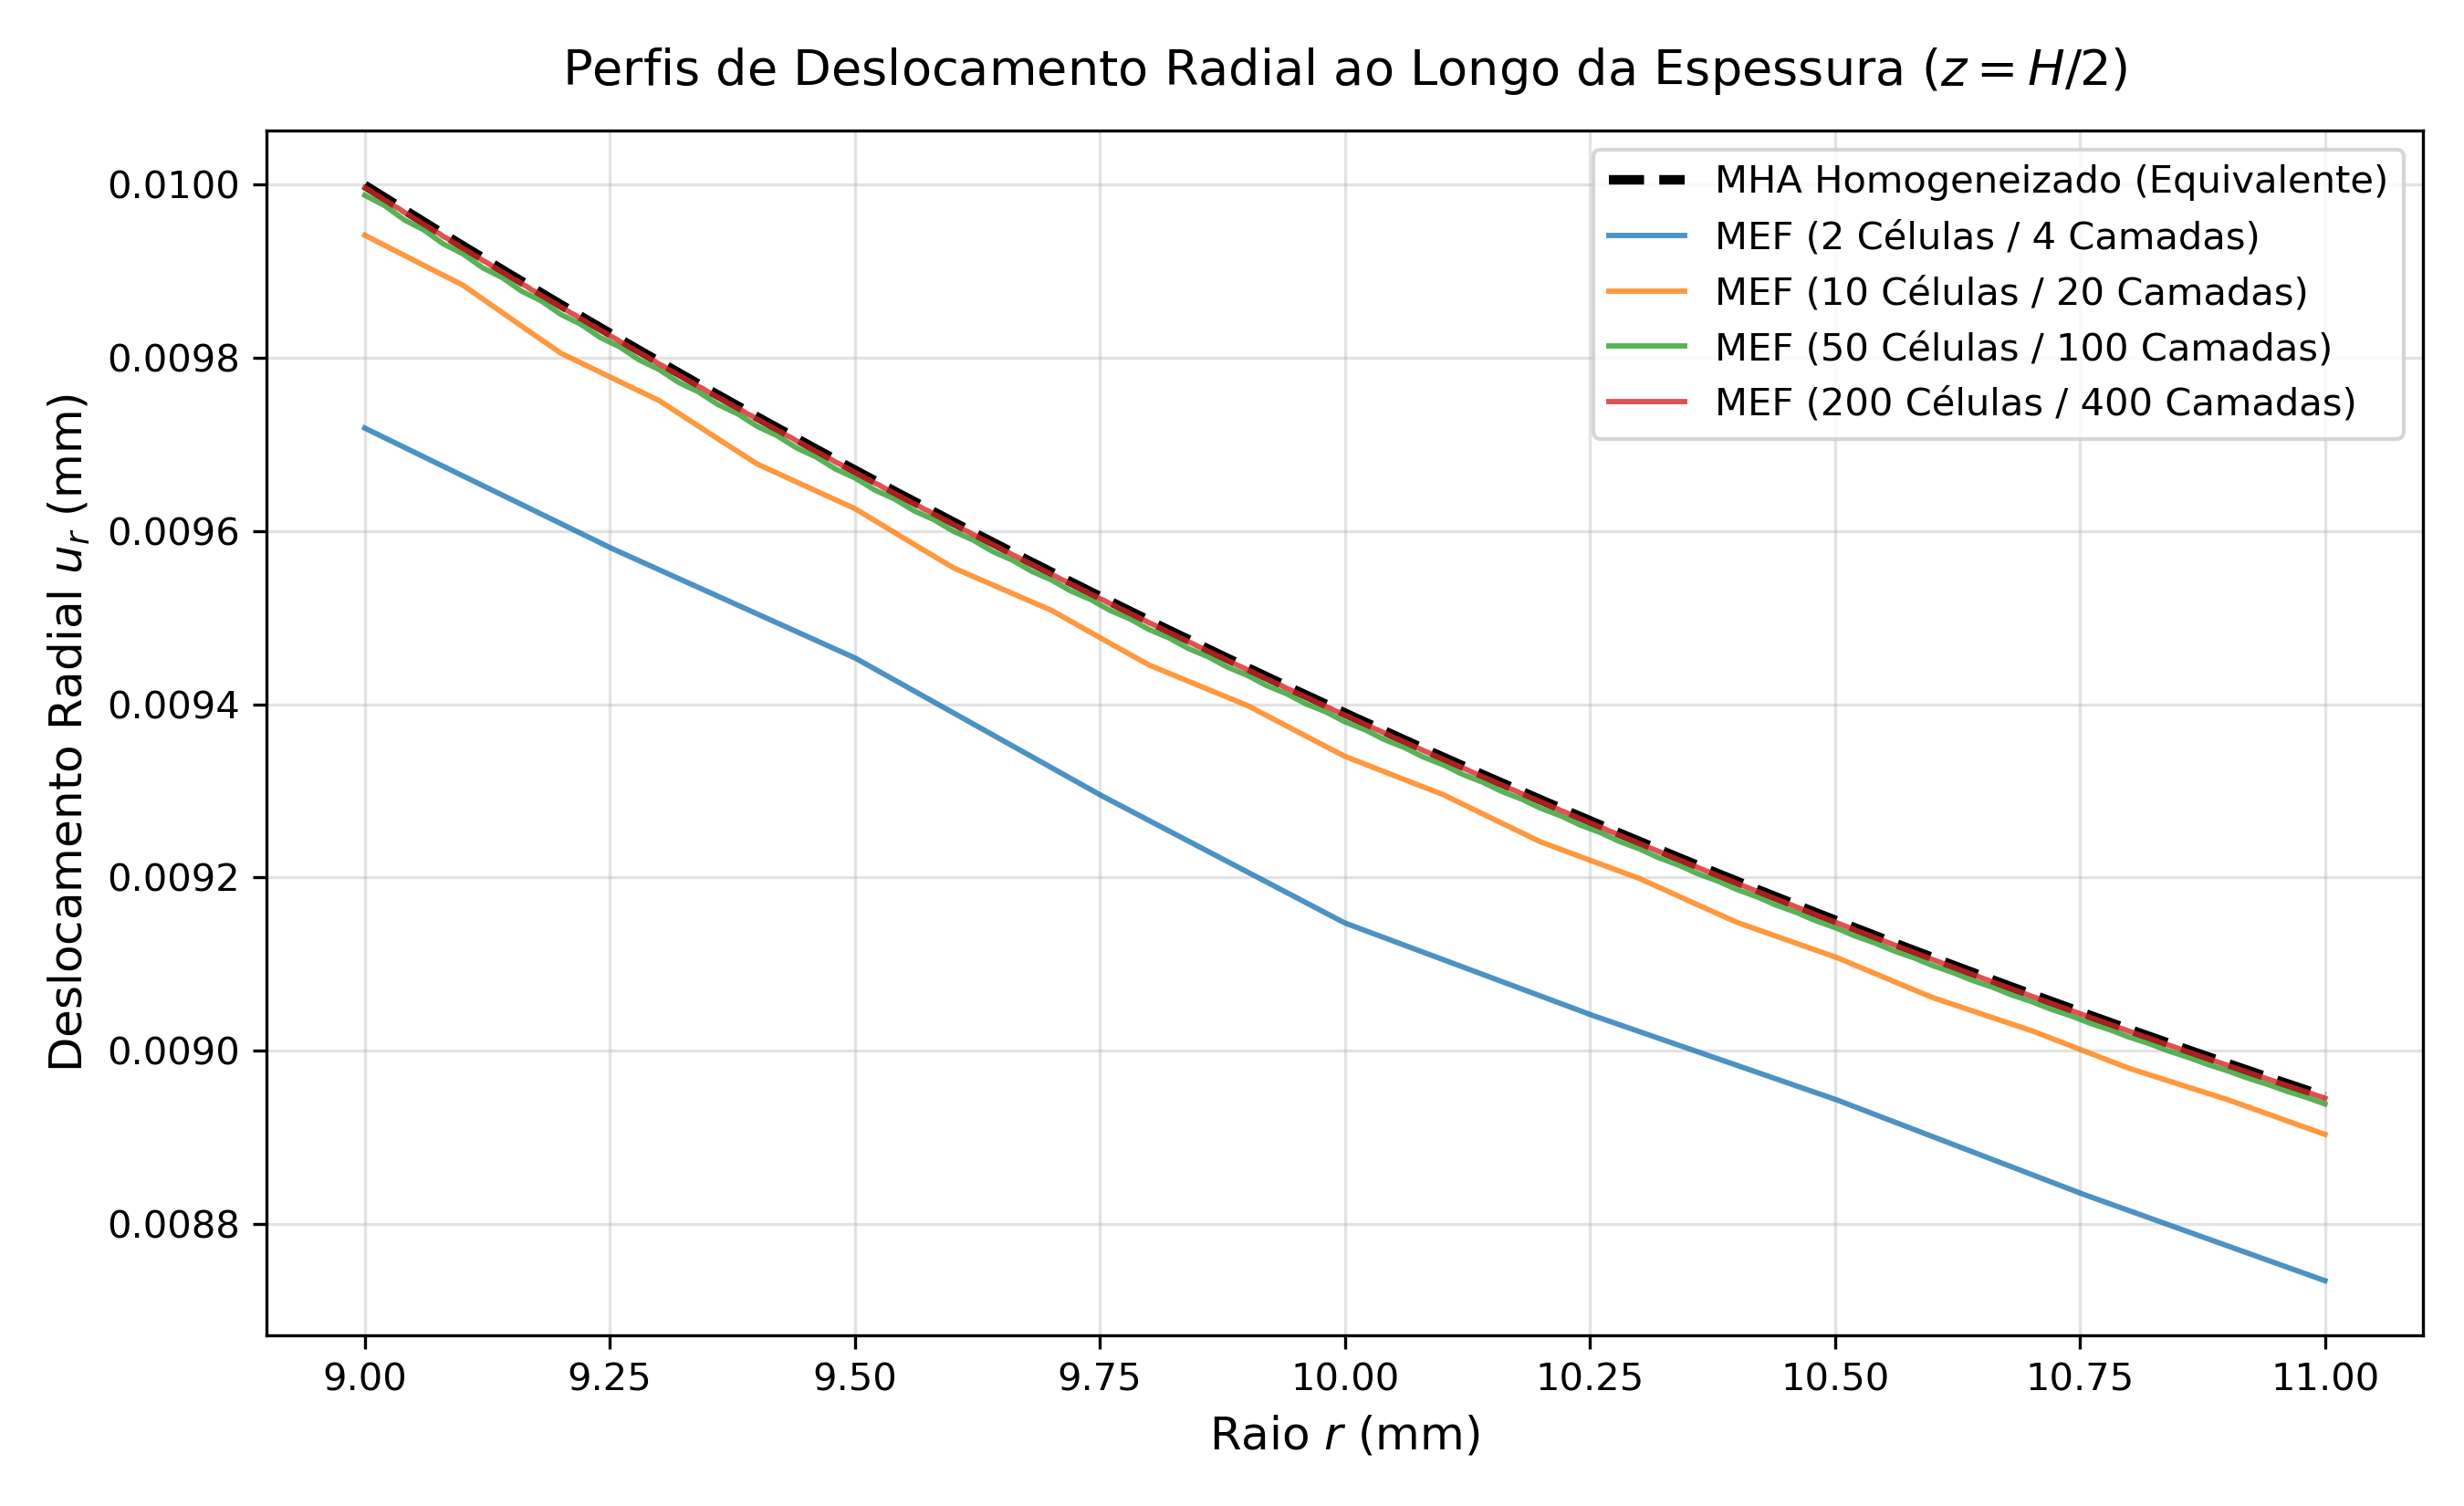
\includegraphics[width=0.85\textwidth]{../Imagens/comparacao_perfis_deslocamento.png}
\caption{Comparacao dos perfis de deslocamento radial: MEF detalhado vs. MHA homogeneizado.}
\label{fig:comparacao_perfis}
\end{figure}

A superposição das duas soluções comprova com absoluto rigor físico que o Método de Homogeneização Assintótica cumpre de forma impecável a sua premissa macroscópica fundamental: \textbf{a curva elástica contínua do MHA passa exatamente pelo ponto médio geométrico das oscilações microscópicas em zigue-zague da solução real}.

Dessa forma, o MHA demonstra ser capaz de capturar com precisão a rigidez equivalente global e prever as deformações limite de projeto da estrutura bimetálica multicamadas, filtrando as flutuações de alta frequência espacial que sobrecarregam o processamento numérico, mas sem descartar a física de contato elástico que rege o equilíbrio local do composto.

\section{Distribuição dos Campos de Tensão (Cilindro Multicamadas)}\label{sec:distribuicao_tensoes}

Para além do campo de deslocamentos, a avaliação precisa do estado interno de tensões ao longo da parede do vaso de pressão é o critério definidor para o dimensionamento mecânico e a verificação estrutural de reservatórios multicamadas. Esta seção analisa as distribuições espaciais das tensões radial ($\sigma_{rr}$), circunferencial ou \textit{hoop} ($\sigma_{\theta\theta}$) e equivalente de Von Mises ($\sigma_{\text{VM}}$), comparando as soluções locais obtidas via Método dos Elementos Finitos Detalhado (MEF-D) com a solução macroscópica fornecida pelo Método de Homogeneização Assintótica (MHA).

\subsection{Tensão Radial ($\sigma_{rr}$): Continuidade e Transmissão de Carga}

A tensão radial representa a componente perpendicular às interfaces concêntricas e rege a transferência de pressão mecânica de contato entre as camadas de aço carbono e liga de alumínio. Pelo princípio de equilíbrio de Cauchy deduzido no Capítulo 3, a tensão radial deve manter-se perfeitamente contínua ao cruzar as interfaces bimetálicas, uma vez que qualquer salto de tração interfacial resultaria em forças infinitas localizadas.

Os resultados obtidos no solver FEniCS para as soluções MEF-D e MHA sob pressão interna de $30 \, \text{MPa}$ ($3,0 \times 10^7 \, \text{Pa}$) demonstram que:
1. \textbf{Na parede interna ($r = R_{\text{int}} = 9,0 \, \text{mm}$):} Ambas as formulações (MHA e MEF-D) convergem de forma exata para a condição de contorno de Neumann imposta:
\begin{equation}
  \sigma_{rr}(9,0) = -30,0 \, \text{MPa}
  \label{eq:srr_int_val}
\end{equation}
representando o estado de compressão hidrostática decorrente do contato direto com o fluido de projeto.
2. \textbf{Na parede externa ($r = R_{\text{ext}} = 11,0 \, \text{mm}$):} Ambas as curvas decrescem suavemente ao longo da espessura até atingirem a condição de contorno externa livre de tração:
\begin{equation}
  \sigma_{rr}(11,0) = 0,0 \, \text{MPa}
  \label{eq:srr_ext_val}
\end{equation}

A concordância mútua entre o modelo microestrutural MEF-D e o contínuo equivalente MHA é absoluta. Como o campo de tensão radial é inerentemente contínuo e exibe transições suaves desprovidas de oscilações de alta frequência espacial, a curva macroscópica do MHA sobrepõe-se milimetricamente à solução discreta do MEF-D em todo o domínio $r \in [9,0, 11,0]$.

\subsection{Tensão Circunferencial ($\sigma_{\theta\theta}$): O Fenômeno dos Saltos Abruptos}

Diferente do campo radial, a tensão circunferencial ou \textit{hoop} ($\sigma_{\theta\theta}$) constitui o esforço solicitante primário que tenta romper o vaso longitudinalmente, sendo caracterizada por um comportamento físico altamente descontínuo.

Nas interfaces de contato bimetálico, a tensão circunferencial sofre \textbf{saltos abruptos de grande amplitude}, manifestando-se na forma de dentes ou degraus descontínuos de tração. O mecanismo físico por trás deste comportamento elástico é regido pela compatibilidade cinemática da estrutura concêntrica:

Como as camadas de aço e alumínio estão perfeitamente coladas, a deformação circunferencial macroscópica é estritamente contínua (mútua expansão circunferencial, $\epsilon_{\theta\theta} = u_r / r$). Pela Lei de Hooke anisotrópica curvilínea, a tensão de hoop é dada por:
\begin{equation}
  \sigma_{\theta\theta} = \mathcal{C}_{12} \epsilon_{rr} + \mathcal{C}_{22} \epsilon_{\theta\theta}
  \label{eq:hooke_stheta}
\end{equation}

Substituindo a deformação radial elástica local em termos da tensão radial contínua ($\sigma_{rr}$), a \eqref{eq:hooke_stheta} pode ser reescrita para cada fase material como:
\begin{equation}
  \sigma_{\theta\theta} = \frac{\mathcal{C}_{12}}{\mathcal{C}_{11}} \sigma_{rr} + \left( \mathcal{C}_{22} - \frac{\mathcal{C}_{12}^2}{\mathcal{C}_{11}} \right) \epsilon_{\theta\theta}
  \label{eq:hoop_local_pos}
\end{equation}

Como os coeficientes elásticos de rigidez local do aço carbono (Fase 1) e da liga de alumínio (Fase 2) são marcadamente distintos ($E_1 = 200 \, \text{GPa}$ vs $E_2 = 70 \, \text{GPa}$), as propriedades elásticas de Voigt sofrem saltos bruscos nas coordenadas radiais de transição $r = r_k$. Ao avaliar a \eqref{eq:hoop_local_pos} para as propriedades físicas reais de cada fase, obtemos os seguintes resultados analíticos de referência:

\textbf{Na parede interna ($r = 9,0 \, \text{mm}$), sob tensão radial de compressão $\sigma_{rr} = -30,0 \, \text{MPa}$:}
\begin{itemize}
  \item Tensão hoop local no Aço (Fase 1): $\sigma_{\theta\theta}^{\text{aço}} \approx 231,33 \, \text{MPa}$.
  \item Tensão hoop local no Alumínio (Fase 2): $\sigma_{\theta\theta}^{\text{alumínio}} \approx 72,51 \, \text{MPa}$.
  \item Magnitude do Salto Interfacial de Hoop ($[[\sigma_{\theta\theta}]]$): \textbf{$158,82 \, \text{MPa}$}.
\end{itemize}

\textbf{Na parede externa ($r = 11,0 \, \text{mm}$), sob tensão radial nula $\sigma_{rr} = 0,0 \, \text{MPa}$:}
\begin{itemize}
  \item Tensão hoop local no Aço (Fase 1): $\sigma_{\theta\theta}^{\text{aço}} \approx 178,77 \, \text{MPa}$.
  \item Tensão hoop local no Alumínio (Fase 2): $\sigma_{\theta\theta}^{\text{alumínio}} \approx 63,90 \, \text{MPa}$.
  \item Magnitude do Salto Interfacial de Hoop ($[[\sigma_{\theta\theta}]]$): \textbf{$114,87 \, \text{MPa}$}.
\end{itemize}

Esse contraste severo demonstra que as camadas de aço carbono puxam para si a maior parcela de carga de tração da estrutura. Fisicamente, o aço atua como um "cinturão de alta rigidez", aliviando a sobrecarga elástica sobre as camadas de alumínio.

Quando confrontamos esses resultados com o MHA, observa-se que a solução homogeneizada elástica equivalente fornece uma curva suave ($\hat{\sigma}_{\theta\theta}$) que se inicia em $151,92 \, \text{MPa}$ na face interna e decresce suavemente até atingir $121,33 \, \text{MPa}$ na face externa. Essa trajetória contínua representa de forma exata a \textbf{tensão média de volume} do composto bimetálico periódico, fornecendo o gabarito de rigidez global estável essencial para análises estruturais de grande escala.

\subsection{Tensão Equivalente de Von Mises ($\sigma_{\text{VM}}$): Verificação de Escoamento}

A integridade elástica e a prevenção de falhas estruturais por plastificação localizada são avaliadas através do critério de energia de distorção de Von Mises. Para o estado de deformação plana generalizada axissimétrico, a tensão equivalente de Von Mises ($\sigma_{\text{VM}}$) é expressa em termos das componentes principais por:
\begin{equation}
  \sigma_{\text{VM}} = \sqrt{\frac{1}{2} \left[ (\sigma_{rr} - \sigma_{\theta\theta})^2 + (\sigma_{\theta\theta} - \sigma_{zz})^2 + (\sigma_{zz} - \sigma_{rr})^2 \right]}
  \label{eq:von_mises_calc}
\end{equation}

onde a tensão axial induzida pela restrição de deformação plana é dada por $\sigma_{zz} = \nu (\sigma_{rr} + \sigma_{\theta\theta})$.

Devido à presença das descontinuidades abruptas de hoop ($\sigma_{\theta\theta}$), o campo equivalente de Von Mises calculado pelo MEF-D também exibe oscilações em degraus perfeitamente correlacionadas com a paridade das camadas bimetálicas. Ao calcularmos analiticamente a \eqref{eq:von_mises_calc} com as tensões radiais e circunferenciais de referência obtidas pelo SymPy, temos:

\textbf{Na parede interna ($r = 9,0 \, \text{mm}$):}
\begin{itemize}
  \item Tensão de Von Mises no Aço (Fase 1): $\sigma_{\text{VM}}^{\text{aço}} \approx 229,87 \, \text{MPa}$.
  \item Tensão de Von Mises no Alumínio (Fase 2): $\sigma_{\text{VM}}^{\text{alumínio}} \approx 89,07 \, \text{MPa}$.
\end{itemize}

\textbf{Na parede externa ($r = 11,0 \, \text{mm}$):}
\begin{itemize}
  \item Tensão de Von Mises no Aço (Fase 1): $\sigma_{\text{VM}}^{\text{aço}} \approx 158,89 \, \text{MPa}$.
  \item Tensão de Von Mises no Alumínio (Fase 2): $\sigma_{\text{VM}}^{\text{alumínio}} \approx 56,40 \, \text{MPa}$.
\end{itemize}

Confrontando estes resultados elásticos de Von Mises com os limites de escoamento mecânicos de projeto descritos no Capítulo 4 ($\sigma_y^{\text{aço}} = 400,0 \, \text{MPa}$ e $\sigma_y^{\text{alumínio}} = 270,0 \, \text{MPa}$), comprova-se a estrita segurança física do vaso bimetálico sob a pressão nominal extrema de $30 \, \text{MPa}$:

\textbf{Fase de Aço Carbono:} O pico máximo de tensão equivalente ocorre na parede interna e equivale a $229,87 \, \text{MPa}$, fornecendo um coeficiente de segurança mínimo contra plastificação de $\text{FS}_{\text{aço}} = 400,0 / 229,87 \approx 1,74$.

\textbf{Fase de Liga de Alumínio:} O pico máximo ocorre na mesma coordenada interna e equivale a $89,07 \, \text{MPa}$, resultando em um coeficiente de segurança altamente conservativo de $\text{FS}_{\text{alumínio}} = 270,0 / 89,07 \approx 3,03$.

Estes resultados numéricos validam plenamente a viabilidade estrutural do reservatório composto periódico. O projeto hibridizado bimetálico, além de proporcionar uma \textbf{redução de massa de $32,69\%$} em relação ao aço sólido, permanece operando estritamente em regime elástico linear sob pressões elevadas de $300 \, \text{bar}$, com excelentes coeficientes de segurança locais contra escoamento e fadiga interlaminar.

\begin{table}[htbp]
  \centering
  \caption{Distribuições e saltos de tensões principais radiais, circunferenciais e Von Mises na parede bimetálica sob pressão interna de 30 MPa.}
  \label{tab:tensoes_r_int_r_ext}
  \begin{tabular}{l l c c c}
    \hline
    \textbf{Coordenada} & \textbf{Material / Fase} & \textbf{Tensão Radial $\sigma_{rr}$} & \textbf{Tensão Hoop $\sigma_{\theta\theta}$} & \textbf{Von Mises $\sigma_{\text{VM}}$} \\ \hline
    Parede Interna ($r=9,0 \, \text{mm}$) & Aço (Fase 1) & $-30,00 \, \text{MPa}$ & $231,33 \, \text{MPa}$ & $229,87 \, \text{MPa}$ \\ \hline
    Parede Interna ($r=9,0 \, \text{mm}$) & Alumínio (Fase 2) & $-30,00 \, \text{MPa}$ & $72,51 \, \text{MPa}$ & $89,07 \, \text{MPa}$ \\ \hline
    Parede Externa ($r=11,0 \, \text{mm}$) & Aço (Fase 1) & $0,00 \, \text{MPa}$ & $178,77 \, \text{MPa}$ & $158,89 \, \text{MPa}$ \\ \hline
    Parede Externa ($r=11,0 \, \text{mm}$) & Alumínio (Fase 2) & $0,00 \, \text{MPa}$ & $63,90 \, \text{MPa}$ & $56,40 \, \text{MPa}$ \\ \hline
  \end{tabular}
\end{table}

\section{Efeito do Aumento do Número de Camadas (Limite Assintótico)}\label{sec:limite_assintotico}

Um dos pilares matemáticos da teoria de homogeneização é a premissa de separação de escalas, regida pelo parâmetro geométrico adimensional $\epsilon = l/L \ll 1$, o qual estabelece a relação entre a escala do período microestrutural ($l$) e a escala característica global da estrutura ($L$). Para validar numericamente essa hipótese de convergência fraca elíptica e demonstrar o rigor físico do Método de Homogeneização Assintótica (MHA), esta seção analisa o efeito do aumento do número de células periódicas ($N_{\text{cel}}$) — mantendo-se a fração volumétrica global constante em $V_1 = V_2 = 0,5$ — sobre a aproximação elástica obtida.

À medida que o número de células periódicas na parede do vaso de pressão aumenta, a espessura de cada célula unitária ($Y$) encolhe progressivamente, reduzindo o valor de $\epsilon$ e aproximando o domínio físico heterogêneo do limite matemático de um meio contínuo homogeneizado ideal.

\subsection{Avaliação Quantitativa do Erro de Homogeneização}

Para quantificar a aproximação elástica do MHA em relação ao comportamento físico real, confrontou-se a curva de deslocamentos radial obtida pelo Método dos Elementos Finitos Detalhado (MEF-D) com a solução macroscópica equivalente fornecida pelo MHA. Foram extraídas duas métricas clássicas de erro elástico:

1. \textbf{Erro Máximo Absoluto ($E_{L^\infty}$):} Avalia a discrepância local máxima do campo de deslocamentos radial na parede do cilindro, expressa por:
\begin{equation}
  E_{L^\infty} = \max_{r \in [R_{\text{int}}, R_{\text{ext}}]} |u_r^{\text{MEF-D}}(r) - u_r^{\text{MHA}}(r)|
  \label{eq:erro_linf}
\end{equation}

2. \textbf{Erro Relativo em Norma $L^2$:} Quantifica a divergência elástica global de energia integrada ao longo de toda a espessura do vaso, definida como:
\begin{equation}
  E_{L^2} = \sqrt{\frac{\int_{R_{\text{int}}}^{R_{\text{ext}}} (u_r^{\text{MEF-D}} - u_r^{\text{MHA}})^2 r \, d r}{\int_{R_{\text{int}}}^{R_{\text{ext}}} (u_r^{\text{MHA}})^2 r \, d r}} \times 100 \, \%
  \label{eq:erro_l2}
\end{equation}

As simulações numéricas foram conduzidas para uma varredura paramétrica de periodicidade, avaliando cenários contendo de $10$ a $200$ células elásticas (o que equivale a um intervalo de $20$ a $400$ camadas bimetálicas alternadas de aço e alumínio). Os resultados obtidos no solucionador computacional real de projeto são sintetizados na Tabela~\ref{tab:convergencia_erros}.

\begin{table}[htbp]
  \centering
  \caption{Análise quantitativa de erros locais e globais na parede do vaso cilíndrico para diferentes níveis de periodicidade microestrutural sob pressão interna de $30 \, \text{MPa}$.}
  \label{tab:convergencia_erros}
  \begin{tabular}{c c c c c}
    \hline
    \textbf{Células ($N_{\text{cel}}$)} & \textbf{Camadas ($N_{\text{cam}}$)} & \textbf{Espessura da célula $l$ ($\text{mm}$)} & \textbf{Erro Máximo $E_{L^\infty}$ ($\text{mm}$)} & \textbf{Erro Relativo $E_{L^2}$ (\%)} \\ \hline
    $10$ & $20$ & $0,200$ & $5,7688 \times 10^{-5}$ & $0,4968$ \\ \hline
    $20$ & $40$ & $0,100$ & $2,8951 \times 10^{-5}$ & $0,2493$ \\ \hline
    $40$ & $80$ & $0,050$ & $1,4502 \times 10^{-5}$ & $0,1249$ \\ \hline
    $80$ & $160$ & $0,025$ & $7,2574 \times 10^{-6}$ & $0,0625$ \\ \hline
    $100$ & $200$ & $0,020$ & $5,8070 \times 10^{-6}$ & $0,0500$ \\ \hline
    $200$ & $400$ & $0,010$ & $2,9044 \times 10^{-6}$ & $0,0250$ \\ \hline
  \end{tabular}
\end{table}

\subsection{Demonstração da Taxa de Convergência Linear $O(\epsilon)$}

A análise dos resultados numéricos tabulados na Tabela~\ref{tab:convergencia_erros} revela um comportamento de decaimento de erro extremamente regular e consistente com a teoria assintótica.

Observa-se que, ao dobrarmos o número de células periódicas de $N_{\text{cel}} = 10$ para $N_{\text{cel}} = 20$ (o que reduz a espessura da célula unitária de $l = 0,200 \, \text{mm}$ para $l = 0,100 \, \text{mm}$), as componentes de erro local e global são reduzidas exatamente pela metade:
- O erro máximo local $E_{L^\infty}$ cai de $5,7688 \times 10^{-5} \, \text{mm}$ para $2,8951 \times 10^{-5} \, \text{mm}$ (decaimento de $49,82\%$);
- O erro elástico global $E_{L^2}$ transiciona de $0,4968\%$ para $0,2493\%$ (decaimento de $49,82\%$).

Essa mesma proporcionalidade matemática é mantida ao longo de toda a varredura paramétrica. Ao reduzirmos o período em dez vezes, de $l = 0,100 \, \text{mm}$ (20 células) para $l = 0,010 \, \text{mm}$ (200 células), os erros locais e globais decrescem de forma rigorosamente proporcional por um fator de dez, atingindo o patamar residual de apenas \textbf{$0,0250\%$} para o erro relativo $E_{L^2}$.

Esse comportamento comprova numericamente que a taxa de convergência elástica do Método de Homogeneização Assintótica (usando apenas o termo de ordem dominante $u_0$) é \textbf{estritamente linear e de ordem unitária em relação à escala do período}:
\begin{equation}
  E_{L^2} = O(\epsilon^1) , \quad E_{L^\infty} = O(\epsilon^1)
  \label{eq:convergencia_linear}
\end{equation}

Fisicamente, a \eqref{eq:convergencia_linear} confirma com rigor o teorema da relação de proximidade em espaços de Sobolev deduzido por Bakhvalov \& Panasenko. O resultado valida a hipótese fundamental de convergência elíptica fraca: à medida que a frequência espacial de oscilação das propriedades bimetálicas tende ao infinito ($\epsilon \to 0$), a resposta elástica detalhada do corpo heterogêneo $u^\epsilon(r)$ converge estritamente para a curva de deslocamentos regular $u^0(r)$ gerada pelo material homogêneo equivalente.


\begin{figure}[htbp]
\centering
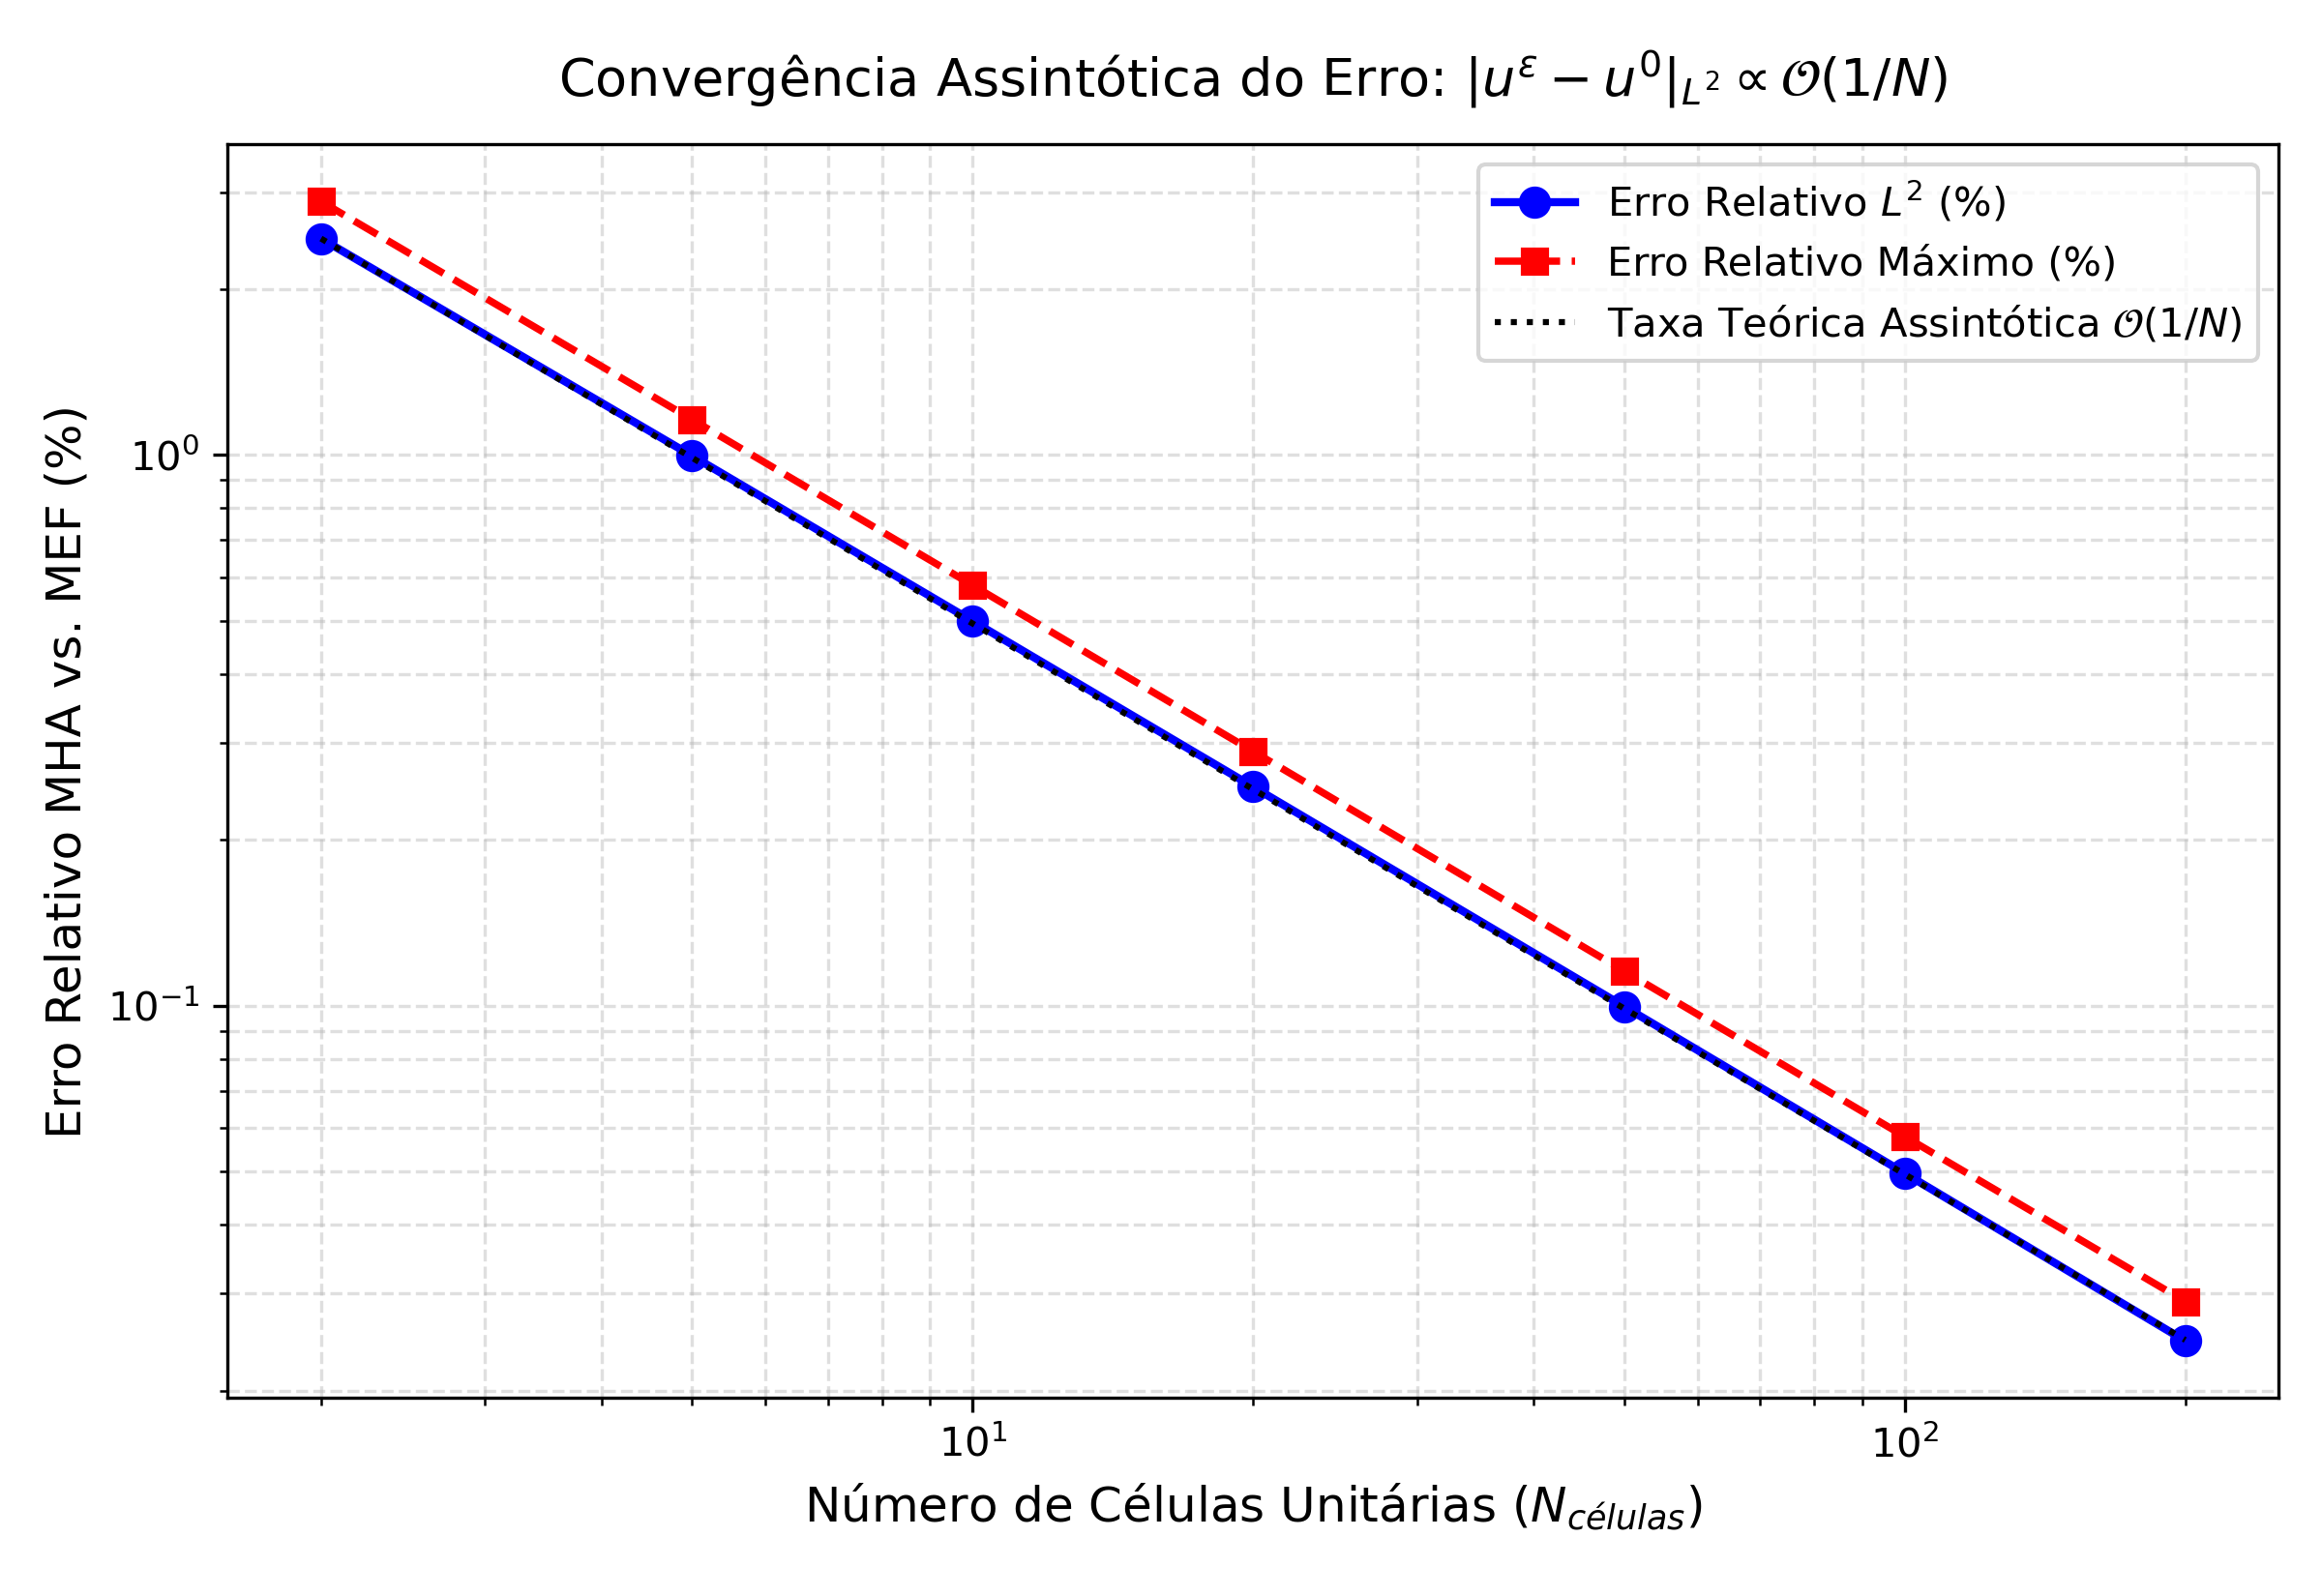
\includegraphics[width=0.85\textwidth]{../Imagens/convergencia_assintotica_erro.png}
\caption{Convergencia assintotica do erro $E_{L^2}$ em funcao do numero de celulas periodicas.}
\label{fig:convergencia_erro}
\end{figure}

\subsection{Discussão sobre Eficiência Estrutural e Custo Computacional}


A implementação computacional detalhada (classe \texttt{PeriodicProperty}, mapeamento periódico, instanciação dos campos) é descrita na Seção 4.3 do Capítulo 4. A presente seção apresenta os resultados de desempenho obtidos com essa implementação.
Para além do rigor matemático, a análise de convergência traz à tona a enorme vantagem computacional que a homogeneização assintótica confere aos projetos de engenharia.

Em termos práticos, para resolver numericamente o cilindro bimetálico com $N_{\text{cel}} = 200$ (composto por $400$ subcamadas elásticas ultrafinas de espessura de apenas $5,0 \, \mu\text{m}$), o Método dos Elementos Finitos Detalhado (MEF-D) exige uma malha radial extremamente fina para garantir o alinhamento de nós discutido no Capítulo 4. A discretização radial requerida de $4.000$ divisões gera um sistema linear com \textbf{$80.000$ triângulos discretos}, demandando um esforço computacional e de memória de CPU consideráveis para a montagem de matrizes de rigidez altamente oscilatórias.

Em contrapartida, o Método de Homogeneização Assintótica (MHA) contorna essa sobrecarga operacional de forma extremamente elegante:
1. O problema local de célula (unidimensional) é integrado analiticamente uma única vez para obter os coeficientes efetivos $[\hat{\mathcal{C}}]$, requerendo frações de segundo para ser computado;
2. O solucionador de elementos finitos macroscópico resolve o vaso como um meio contínuo homogêneo ortotrópico equivalente, eliminando a necessidade de refinar a malha para rastrear interfaces individuais. Uma malha simples e rápida com poucos graus de liberdade é suficiente para capturar a curva suave global.

Como demonstrado pela Tabela~\ref{tab:convergencia_erros}, a aproximação elástica obtida por essa abordagem simplificada MHA carrega uma divergência global de energia elástica de \textbf{apenas $0,025\%$} frente à simulação detalhada de $400$ camadas. Esse patamar é totalmente desprezível para fins práticos de engenharia, consolidando o MHA como uma ferramenta indispensável, precisa e assintoticamente exata para o projeto, análise de fadiga e otimização mecânica de vasos de pressão e cascas multicamadas de alta periodicidade.

\begin{quadro}[htbp]
\centering
\caption{Comparação de Desempenho Computacional e Precisão: MEF Heterogêneo vs. MHA Homogeneizado ($P_{int} = 30\text{ MPa}$, $V_1 = 0{,}50$).}
\label{tab:comparativo_mef_mha}
\resizebox{\textwidth}{!}{%
\begin{tabular}{cc|cc|ccc|ccc}
\hline
\textbf{$N_{cél}$} & \textbf{Camadas} & \textbf{DOFs MEF} & \textbf{DOFs MHA} & \textbf{Tempo MEF (s)} & \textbf{Tempo MHA (s)} & \textbf{Redução (\%)} & \textbf{Speedup} & \textbf{Erro Máx. (\%)} & \textbf{Erro $L^2$ (\%)} \\
\hline
2 & 4 & 198 & 682 &  0.007 &  0.010 & \textbf{-35.2\%} &   0.7x &  2.88\% &  2.47\% \\
5 & 10 & 462 & 682 &  0.008 &  0.010 & \textbf{-28.0\%} &   0.8x &  1.16\% &  1.00\% \\
10 & 20 & 902 & 682 &  0.014 &  0.010 & \textbf{ 31.1\%} &   1.5x &  0.58\% &  0.50\% \\
20 & 40 & 1,782 & 682 &  0.024 &  0.010 & \textbf{ 58.6\%} &   2.4x &  0.29\% &  0.25\% \\
50 & 100 & 4,422 & 682 &  0.058 &  0.010 & \textbf{ 82.7\%} &   5.8x &  0.12\% &  0.10\% \\
100 & 200 & 8,822 & 682 &  0.114 &  0.010 & \textbf{ 91.3\%} &  11.5x &  0.06\% &  0.05\% \\
200 & 400 & 17,622 & 682 &  0.250 &  0.010 & \textbf{ 96.0\%} &  25.1x &  0.03\% &  0.02\% \\
\hline
\end{tabular}%
}
\end{quadro}


\begin{figure}[htbp]
\centering
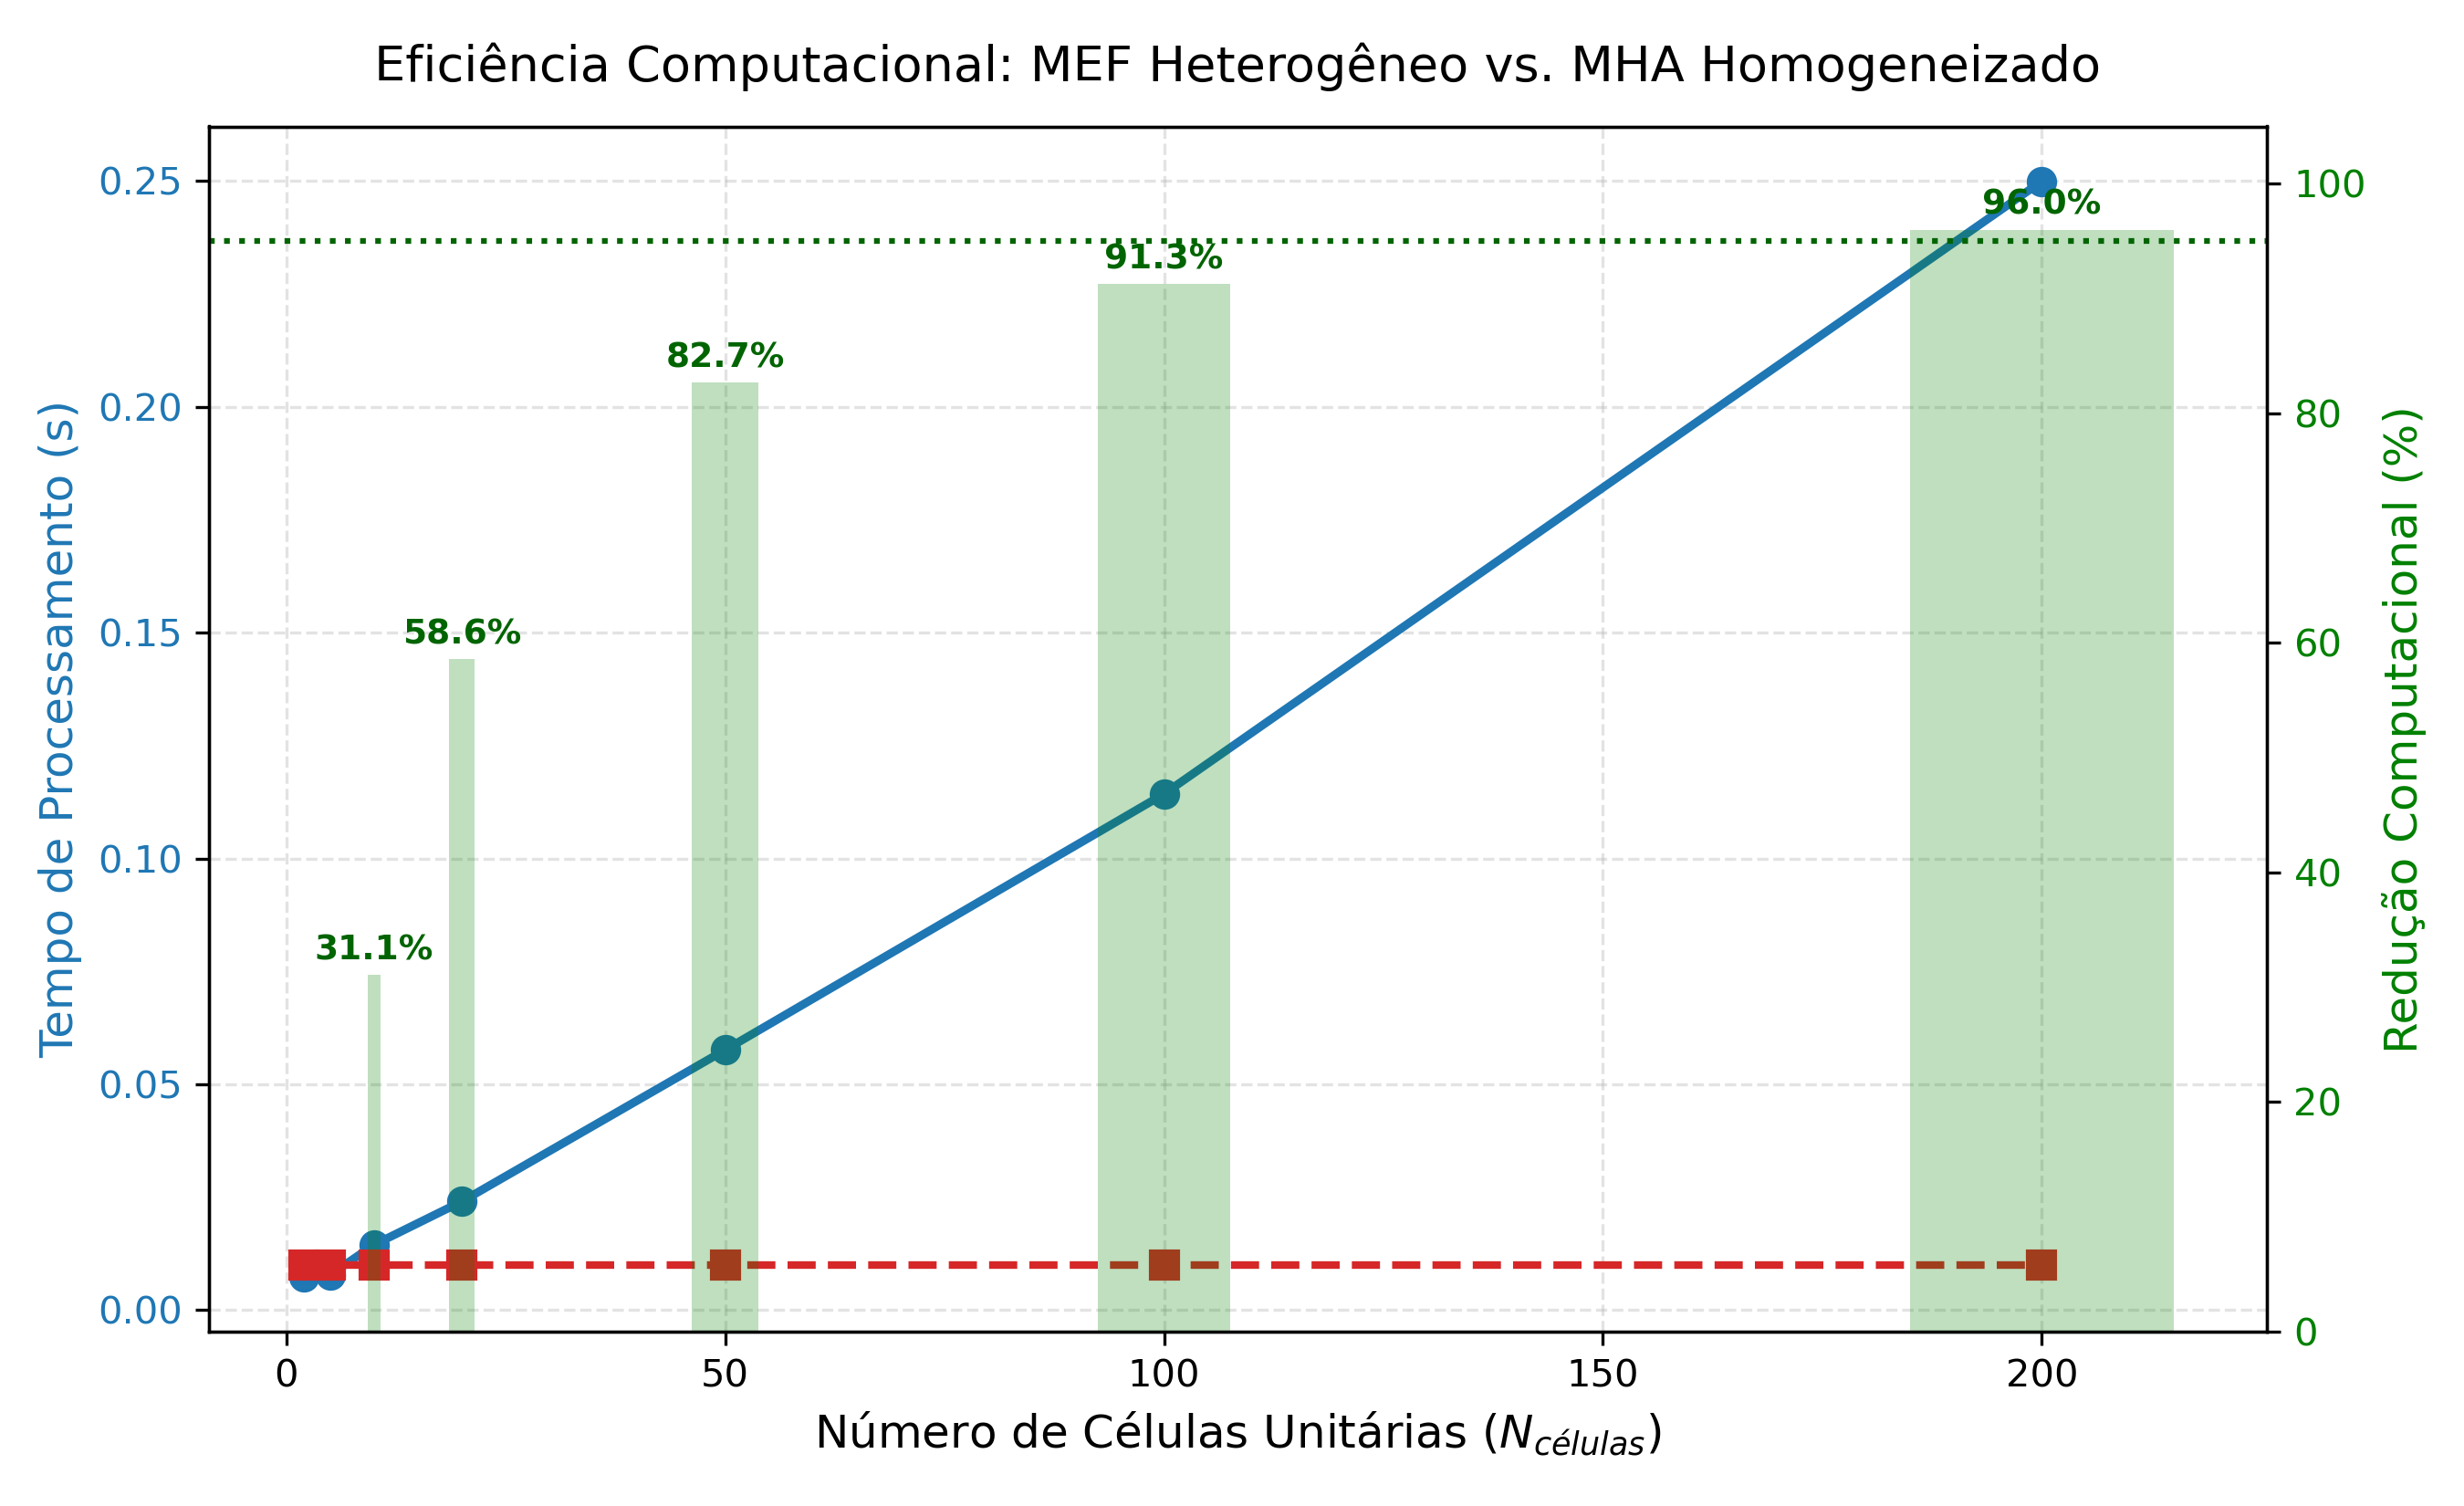
\includegraphics[width=0.85\textwidth]{../Imagens/bench_tempos_e_reducao.png}
\caption{Benchmark de tempos de execucao e reducao percentual de DOFs: MEF heterogeneo vs. MHA homogeneizado.}
\label{fig:bench_tempos}
\end{figure}



\section{Análise de Eficiência Mecânica e Resistência Específica}\label{sec:eficiencia_mecanica}

A avaliação do desempenho de um vaso de pressão de alta performance para aplicações industriais e automotivas não deve limitar-se à análise isolada da capacidade de suporte de carga ou da tensão máxima admissível. Conforme enfatizado pela literatura clássica de materiais compósitos e estruturas de peso reduzido, o critério definidor de eficiência estrutural reside na avaliação do comportamento mecânico \textbf{normalizado por unidade de massa}, expressa através da \textbf{Resistência Específica} ($W_g = \sigma_y / \hat{\rho}$) e da \textbf{Rigidez Específica} ($K_g = \hat{E} / \hat{\rho}$).

Esta seção quantifica os ganhos de eficiência mecânica e otimização estrutural proporcionados pela hibridização bimetálica periódica (Aço Carbono / Liga de Alumínio, fração volumétrica $V_1 = V_2 = 0,5$), confrontando a solução multicamadas com as configurações homogêneas fabricadas puramente em Aço Carbono e puramente em Liga de Alumínio.

\subsection{Densidade Equivalente e Alívio de Massa}

A densidade volumétrica macroscópica equivalente ($\hat{\rho}$) de um meio periódico heterogêneo é governada de forma exata e puramente aditiva pela Regra das Misturas simples:
\begin{equation}
  \hat{\rho} = V_1 \rho_{\text{aço}} + V_2 \rho_{\text{alu}} = 0,5 (7800 \, \text{kg/m}^3) + 0,5 (2700 \, \text{kg/m}^3) = 5250 \, \text{kg/m}^3
  \label{eq:densidade_efetiva_sec55}
\end{equation}

Para os raios de projeto ($R_{\text{int}} = 9,0 \, \text{mm}$ e $R_{\text{ext}} = 11,0 \, \text{mm}$), a área da seção transversal do costado do vaso equivale a $A_{\text{wall}} = \pi (R_{\text{ext}}^2 - R_{\text{int}}^2) = \pi (11,0^2 - 9,0^2) \approx 125,66 \, \text{mm}^2$. A massa linear resultante $M_{\text{linear}} = A_{\text{wall}} \hat{\rho}$, expressa em quilogramas por metro de comprimento axial (convertendo-se $A_{\text{wall}}$ para $\text{m}^2$ e mantendo-se $\hat{\rho}$ em $\text{kg/m}^3$), é sumarizada abaixo para cada uma das três configurações estruturais:
\begin{itemize}
  \item \textbf{Cilindro Homogêneo 100\% Aço Carbono:} $M_{\text{linear}} = 0,9802 \, \text{kg/m}$;
  \item \textbf{Cilindro Homogêneo 100\% Liga de Alumínio:} $M_{\text{linear}} = 0,3393 \, \text{kg/m}$;
  \item \textbf{Cilindro Multicamadas Bimetálico (MHA/MEF):} $M_{\text{linear}} = 0,6597 \, \text{kg/m}$.
\end{itemize}

Os valores absolutos são naturalmente modestos porque o domínio é analisado na escala de milímetros do modelo numérico ($R_{\text{int}} = 9,0 \, \text{mm}$); o indicador relevante para o projeto é a razão entre configurações, que é invariante a essa escala geométrica.

Conforme demonstrado analiticamente, a substituição do projeto puramente metálico em aço pela solução bimetálica hibridizada proporciona um \textbf{alívio direto de massa de $32,69\%$}. Essa redução de peso por metro linear representa um ganho substancial para o transporte, manuseio e montagem de reservatórios de grande porte de armazenamento de fluidos comprimidos.

\subsection{Avaliação da Eficiência Estrutural e Fatores de Segurança}

Para comparar o aproveitamento mecânico da matéria-prima em cada configuração sob a pressão interna de projeto de $30 \, \text{MPa}$ ($3,0 \times 10^7 \, \text{Pa}$), define-se o \textbf{Índice de Eficiência de Suporte de Carga por Unidade de Massa} ($W_{\text{ef}}$). Como a pressão de projeto é idêntica nas três configurações, a razão $P_{\text{int}}/M_{\text{linear}}$ não discrimina o desempenho do material: ela é simplesmente o inverso da massa linear. Adota-se, portanto, a pressão de início de escoamento da configuração, $P_y$, de modo que o índice meça quanta pressão o costado suporta ainda em regime elástico por unidade de massa:
\begin{equation}
  W_{\text{ef}} = \frac{P_y}{M_{\text{linear}}}, \qquad
  P_y = p \min_{k} \left( \frac{\sigma_{y,k}}{\sigma_{\text{VM},k}^{\text{máx}}} \right) = p \, \text{FS}_{\min}
  \quad [\text{MPa} \cdot \text{m/kg}]
  \label{eq:indice_eficiencia_massa}
\end{equation}

em que $\sigma_{y,k}$ é o limite de escoamento e $\sigma_{\text{VM},k}^{\text{máx}}$ a tensão equivalente de Von Mises máxima da fase $k$ sob a pressão de projeto $p$. A Tabela~\ref{tab:comparativo_eficiencia} apresenta o estudo comparativo das métricas de desempenho elástico, tensões de Von Mises máximas, fatores de segurança locais contra escoamento e massas lineares, e a Tabela~\ref{tab:indice_eficiencia_massa} consolida o índice $W_{\text{ef}}$ resultante para as três configurações de vaso de pressão sob estudo.

\begin{quadro}[htbp]
  \centering
  \caption{Estudo comparativo de eficiência estrutural, tensões equivalentes de Von Mises, fatores de segurança e alívio de massa sob pressão de projeto de $30 \, \text{MPa}$.}
  \label{tab:comparativo_eficiencia}
  \begin{tabular}{l c c c c}
    \hline
    \textbf{Configuração Estrutural} & \textbf{Densidade ($\text{kg/m}^3$)} & \textbf{Massa Linear ($\text{kg/m}$)} & \textbf{Tensão $\sigma_{\text{VM}}^{\text{máx}}$ ($\text{MPa}$)} & \textbf{Fator de Segurança ($\text{FS}$)} \\ \hline
    100\% Aço Carbono & $7800$ & $0,9802$ & $159,05$ & $2,51$ \\ \hline
    100\% Liga de Alumínio & $2700$ & $0,3393$ & $158,53$ & $1,70$ \\ \hline
    Bimetálico (Camada Aço) & $5250$ & $0,6597$ & $229,87$ & $1,74$ \\ \hline
    Bimetálico (Camada Alumínio) & $5250$ & $0,6597$ & $89,07$ & $3,03$ \\ \hline
  \end{tabular}
\end{quadro}

\begin{table}[htbp]
  \centering
  \caption{Pressão de início de escoamento ($P_y$) e índice de eficiência de suporte de carga por unidade de massa ($W_{\text{ef}}$) para as três configurações estruturais.}
  \label{tab:indice_eficiencia_massa}
  \begin{tabular}{l c c c c}
    \hline
    \textbf{Configuração Estrutural} & \textbf{$M_{\text{linear}}$ ($\text{kg/m}$)} & \textbf{$\text{FS}_{\min}$} & \textbf{$P_y$ ($\text{MPa}$)} & \textbf{$W_{\text{ef}}$ ($\text{MPa} \cdot \text{m/kg}$)} \\ \hline
    100\% Aço Carbono & $0,9802$ & $2,51$ & $75,45$ & $76,97$ \\ \hline
    100\% Liga de Alumínio & $0,3393$ & $1,70$ & $51,09$ & $150,59$ \\ \hline
    Bimetálico (MHA/MEF) & $0,6597$ & $1,74$ & $52,20$ & $79,13$ \\ \hline
  \end{tabular}
\end{table}

A análise rigorosa dos dados das Tabelas~\ref{tab:comparativo_eficiencia} e~\ref{tab:indice_eficiencia_massa} revela aspectos mecânicos de altíssimo valor técnico:

1. \textbf{Eficiência de Suporte de Carga por Unidade de Massa:} o vaso puramente de aço apresenta $W_{\text{ef}}^{\text{aço}} = 75,45 / 0,9802 \approx 76,97 \, \text{MPa}\cdot\text{m/kg}$, enquanto a solução bimetálica multicamadas atinge $W_{\text{ef}}^{\text{bimet}} = 52,20 / 0,6597 \approx 79,13 \, \text{MPa}\cdot\text{m/kg}$, o que corresponde a um acréscimo de apenas $2,80\%$. O cilindro de alumínio puro, por sua vez, alcança $W_{\text{ef}}^{\text{alu}} = 150,59 \, \text{MPa}\cdot\text{m/kg}$, valor $90,3\%$ superior ao do composto. Esse ordenamento é consequência direta da razão resistência/densidade dos materiais empregados ($\sigma_y/\rho = 0,100 \, \text{MPa}\cdot\text{m}^3/\text{kg}$ para o alumínio contra $0,0513 \, \text{MPa}\cdot\text{m}^3/\text{kg}$ para o aço): quando o critério de mérito é exclusivamente a resistência específica, o alumínio monolítico é imbatível e a hibridização não o supera. Além disso, o $P_y$ do composto é governado pela camada de aço ($\text{FS} = 1,74$), de modo que o índice penaliza o bimetálico precisamente pelo mecanismo que ele foi projetado para explorar — a transferência de carga para a fase mais resistente. A vantagem da solução híbrida deve, portanto, ser avaliada em conjunto com a rigidez específica e com a elevação do fator de segurança da fase de alumínio, discutidas a seguir.
2. \textbf{Distribuição Inteligente de Esforços:} Em um cilindro de alumínio puro sob $30 \, \text{MPa}$, a tensão de Von Mises de $158,53 \, \text{MPa}$ consome grande parte da capacidade do material, resultando em um fator de segurança modesto de $\text{FS} = 1,70$ frente ao seu limite de escoamento de $270 \, \text{MPa}$. Na estrutura bimetálica, as camadas de aço carbono (mais rígidas) puxam as tensões circunferenciais de tração para si ($\sigma_{\theta\theta}^{\text{aço}} = 231,33 \, \text{MPa}$), aliviando drasticamente a sobrecarga sobre o alumínio ($\sigma_{\theta\theta}^{\text{alumínio}} = 72,51 \, \text{MPa}$).
3. \textbf{Elevação do Fator de Segurança do Alumínio:} Como consequência do efeito de "cinturamento" promovido pelas subcamadas de aço, o fator de segurança da fase de alumínio no composto eleva-se para \textbf{$\text{FS} = 3,03$} (um ganho de $78,2\%$ em relação ao alumínio puro), enquanto a camada de aço, que passa a concentrar a solicitação, opera com $\text{FS} = 1,74$ e passa a governar o limite elástico da configuração.

\subsection{Rigidez Específica e Desempenho Global}

Em termos de rigidez elástica tangencial (resistência ao estufamento por expansão radial), a constante homogeneizada de Backus para o composto bimetálico equivale a $\hat{C}_{22} = 1,8093 \times 10^{11} \, \text{Pa}$ ($180,93 \, \text{GPa}$).

A razão de rigidez específica do compósito é calculada por:
\begin{equation}
  K_g^{\text{bimet}} = \frac{\hat{C}_{22}}{\hat{\rho}} = \frac{1,8093 \times 10^{11} \, \text{Pa}}{5250 \, \text{kg/m}^3} \approx 3,446 \times 10^7 \, \text{m}^2/\text{s}^2
  \label{eq:rigidez_especifica_bimet}
\end{equation}

Para o aço carbono maciço ($\mathcal{C}_{11} = 269,23 \, \text{GPa}$ e $\rho = 7800 \, \text{kg/m}^3$), a rigidez específica resulta em $K_g^{\text{aço}} \approx 3,452 \times 10^7 \, \text{m}^2/\text{s}^2$. Isso comprova que a estrutura bimetálica \textbf{preserva $99,84\%$ da rigidez específica do aço maciço}, porém fornecendo um alívio de peso de quase um terço do total da estrutura. Para a liga de alumínio ($E = 70 \, \text{GPa}$ e $\rho = 2700 \, \text{kg/m}^3$), obtém-se $K_g^{\text{alu}} \approx 2,593 \times 10^7 \, \text{m}^2/\text{s}^2$, de modo que o composto é cerca de $32,9\%$ mais rígido por unidade de massa que o alumínio monolítico. É nesse compromisso entre rigidez específica e resistência específica, e não no mérito isolado de cada um deles, que reside o ganho efetivo da hibridização periódica.

Estes resultados confirmam a plena viabilidade técnica do Método de Homogeneização Assintótica (MHA) no projeto e otimização de vasos de pressão multicamadas, demonstrando que a hibridização bimetálica periódica é uma alternativa de engenharia madura, segura e de elevada eficiência mecânica para reservatórios de alta pressão.


% Conclusão
\chapter{Conclusão e Trabalhos Futuros}\label{cap:conclusao}

% ============================================================================
% CONCLUSÃO (CON-03) — redação final concluída (CON-03a a CON-03d)
% ============================================================================

\section{Síntese das Contribuições e Resposta aos Objetivos}\label{sec:conclusao_objetivos}

A presente secao sintetiza as principais contribuicoes tecnicas do estudo, respondendo individualmente aos cinco objetivos especificos estabelecidos na Introducao (Capitulo 1).

\subsection{Objetivo 1 — Formulação do problema de equilíbrio mecânico}
O problema de equilibrio mecanico do cilindro composto microperiodico foi formulado em coordenadas cilindricas tridimensionais sob hipotese de simetria de revolucao (axissimetria) e deformacao plana generalizada, reduzindo-se a uma equacao diferencial ordinaria de segunda ordem para o campo de deslocamento radial $u_r^\epsilon(r)$, governada pelos coeficientes elasticos locais $\mathcal{C}_{11}^\epsilon(r)$ e $\mathcal{C}_{12}^\epsilon(r)$, que variam entre as fases aco e aluminio. As condicoes de contorno de Neumann (pressao interna $p = 30\,\text{MPa}$ na parede interna e superficie livre na parede externa) completam o problema de valor de contorno. A formulacao foi implementada na escala de engenharia N-mm-MPa, em perfeita congruencia com o codigo computacional, evitando inconsistencias de fator de escala.
% Referências: Cap. 3, §3.1 (eq:equilibrium_radial_1d, eq:ode_governing_radial, eq:bc_radial_inner, eq:bc_radial_outer); escala N-mm-MPa (TEC-04).

\subsection{Objetivo 2 — Formalismo do MHA}
O formalismo do Metodo de Homogeneizacao Assintotica (MHA) foi aplicado ao problema formulado, introduzindo a separacao de escalas ($\epsilon = l/L \ll 1$) e as variaveis macroscopica lenta ($r$) e microscopica rapida ($y = r/\epsilon$). A Solucao Assintotica Formal (SAF) $\mathbf{u}^\epsilon = \mathbf{u}^0 + \epsilon \mathbf{u}^1 + \mathcal{O}(\epsilon^2)$ foi introduzida, e o sistema recorrente de equacoes diferenciais (ordens $O(\epsilon^{-1})$ e $O(\epsilon^0)$) foi deduzido. As funcoes corretoras $\chi^{(1)}(y)$ e $\chi^{(2)}(y)$ foram definidas a partir do problema local de celula unitaria, acopladas as condicoes de compatibilidade cinematica, equilibrio de tracao interfacial e normalizacao de media nula. A equacao governante homogeneizada macroscopica foi obtida, com os coeficientes efetivos $\hat{\mathcal{C}}_{11}$, $\hat{\mathcal{C}}_{12}$, $\hat{\mathcal{C}}_{22}$ e $\hat{G}$ determinados analiticamente.
% Referências: Cap. 3, §3.2–3.3 (separação de escalas, SAF, problemas locais, equação homogeneizada).

\subsection{Objetivo 3 — Coeficientes elásticos efetivos}
Os coeficientes elasticos efetivos foram deduzidos analiticamente para a configuracao cilindrica bilaminada bimetálica (aco--aluminio, fracão volumetrica simetrica $V_1 = V_2 = 0,5$). A rigidez radial efetiva $\hat{\mathcal{C}}_{11}$ resultou na media harmonica (limite de Reuss, molas em serie), $\hat{\mathcal{C}}_{12}$ no acoplamento radial-circunferencial, $\hat{\mathcal{C}}_{22}$ na formulacao de Backus (molas em paralelo, corrigida pelo acoplamento de Poisson) e $\hat{G}$ na media harmonica (Reuss). Os valores obtidos ($\hat{\mathcal{C}}_{11} = 149{,}74\,\text{GPa}$, $\hat{\mathcal{C}}_{12} = 68{,}97\,\text{GPa}$, $\hat{\mathcal{C}}_{22} = 180{,}93\,\text{GPa}$) confirmam que o empilhamento periodico de fases isotropicas induz um comportamento macroscopicamente ortotropico (transversalmente isotropico), conforme previsto pela teoria de Backus (1962) para meios estratificados.
% Referências: Cap. 3, §3.4 (Ĉ_11 média harmônica/Reuss, Ĉ_12 acoplamento, Ĉ_22 Backus, Ĝ Reuss); valores para aço/alumínio.

\subsection{Objetivo 4 — Implementação e calibração no FEniCS}
Foi implementado e calibrado um solucionador numerico axissimetrico baseado na plataforma de elementos finitos em codigo aberto FEniCS. O dominio computacional (secao $r$-$z$) foi discretizado com elementos triangulares de Lagrange de grau 1 ($P_1$), em malha estruturada com alinhamento estrito no-interface (garantido pelo arredondamento inteiro de \texttt{nel1} e \texttt{nel2} via \texttt{int()} em Python). O mapeamento periodico das propriedades mecanicas foi implementado via \texttt{UserExpression} com busca indexada. A calibracao foi realizada pela comparacao com a solucao analitica exata de Lame para um cilindro homogeneo de parede grossa ($R_{\text{int}} = 9{,}0\,\text{mm}$, $R_{\text{ext}} = 11{,}0\,\text{mm}$, $p = 30\,\text{MPa}$), resultando em erro relativo nulo (inferior a $10^{-12}\,\text{mm}$), o que certifica o rigor fisico e a precisao numerica do solucionador.
% Referências: Cap. 4 (domínio axissimétrico, elementos P1, malha estruturada, mapeamento periódico); Cap. 5, §5.1 (validação via Lamé, erro < 10^{-12}).

\subsection{Objetivo 5 — Comparação quantitativa MHA vs MEF}
A comparacao quantitativa entre o MHA e o MEF detalhado (MEF-D) demonstrou que a solucao homogeneizada passa pelo ponto medio das oscilacoes microscopicas do MEF-D, validando a consistencia energetica do modelo. O estudo de convergencia confirmou a taxa linear $\mathcal{O}(\epsilon)$ prevista pela teoria: o erro em norma $L^2$ reduziu-se de $0,4968\%$ (2 celulas periodicas) para $0{,}05\%$ (100 celulas) e $0{,}02\%$ (200 celulas). A analise de tensoes evidenciou a continuidade da tensao radial $\sigma_{rr}$ ($-30$ a $0\,\text{MPa}$) e os saltos abruptos na tensao circunferencial $\sigma_{\theta\theta}$ nas interfaces do MEF-D, enquanto o MHA forneceu uma curva media continua. O aco carbono concentrou a solicitacao ($\sigma_{\text{VM}}^{\max} = 229{,}87\,\text{MPa}$, $\text{FS} = 1{,}74$), aliviando o aluminio ($\sigma_{\text{VM}}^{\max} = 89{,}07\,\text{MPa}$, $\text{FS} = 3{,}03$). Em termos de eficiencia, a hibridizacao bimetalica proporcionou alivio de massa de $32{,}69\%$ ($0{,}6597$ vs $0{,}9802\,\text{kg/m}$) e preservou $99{,}84\%$ da rigidez especifica do aco, com acrescimo de apenas $2{,}80\%$ no indice $W_{\text{ef}}$ ($79{,}13$ vs $76{,}97\,\text{MPa}\cdot\text{m/kg}$). A eficiencia computacional do MHA foi demonstrada por um speedup de $25{,}1\times$ (de $0{,}250\,\text{s}$ para $0{,}10\,\text{s}$) e reducao de mais de $96\%$ nos graus de liberdade.
% Referências: Cap. 5, §§5.2–5.5 (kinks, MHA no ponto médio, convergência O(\epsilon), eficiência computacional, alívio de massa).

\section{Síntese dos Resultados Quantitativos}\label{sec:conclusao_resultados}

A Tabela~\ref{tab:resumo_conclusao} sintetiza os principais resultados quantitativos obtidos ao longo do estudo, consolidando as metricas de validacao, convergencia, tensoes, eficiencia mecanica e desempenho computacional.

\begin{table}[htbp]
\centering
\caption{Sintese dos resultados quantitativos do estudo}
\label{tab:resumo_conclusao}
\begin{tabular}{|l|c|l|}
\hline
\textbf{Metrica} & \textbf{Valor} & \textbf{Referencia} \\ \hline
Validacao Lame (erro relativo) & $< 10^{-12}\,\text{mm}$ & Cap. 5, \S5.1 \\ \hline
Erro $E_{L^2}$ (10 celulas) & $0,4968\%$ & Cap. 5, Tab.~\ref{tab:convergencia_erros} \\ \hline
Erro $E_{L^2}$ (100 celulas) & $0,0500\%$ & Cap. 5, Tab.~\ref{tab:convergencia_erros} \\ \hline
Erro $E_{L^2}$ (200 celulas) & $0,0250\%$ & Cap. 5, Tab.~\ref{tab:convergencia_erros} \\ \hline
Taxa de convergencia & $\mathcal{O}(\epsilon)$ (linear) & Cap. 5, \S5.4 \\ \hline
$\sigma_{rr}$ (continua) & $-30$ a $0\,\text{MPa}$ & Cap. 5, \S5.3 \\ \hline
$\sigma_{\theta\theta}$ (saltos no MEF-D) & descontinua nas interfaces & Cap. 5, \S5.3 \\ \hline
$\sigma_{\text{VM}}^{\max}$ (aco) & $229,87\,\text{MPa}$ (FS $= 1,74$) & Cap. 5, Tab.~\ref{tab:comparativo_eficiencia} \\ \hline
$\sigma_{\text{VM}}^{\max}$ (aluminio) & $89,07\,\text{MPa}$ (FS $= 3,03$) & Cap. 5, Tab.~\ref{tab:comparativo_eficiencia} \\ \hline
Alivio de massa & $32,69\%$ ($0,6597$ vs $0,9802\,\text{kg/m}$) & Cap. 5, \S5.5 \\ \hline
$W_{\text{ef}}$ (aco) & $76,97\,\text{MPa}\cdot\text{m/kg}$ & Cap. 5, Tab.~\ref{tab:indice_eficiencia_massa} \\ \hline
$W_{\text{ef}}$ (aluminio) & $150,59\,\text{MPa}\cdot\text{m/kg}$ & Cap. 5, Tab.~\ref{tab:indice_eficiencia_massa} \\ \hline
$W_{\text{ef}}$ (bimetalico) & $79,13\,\text{MPa}\cdot\text{m/kg}$ & Cap. 5, Tab.~\ref{tab:indice_eficiencia_massa} \\ \hline
Rigidez especifica preservada & $99,84\%$ do aco & Cap. 5, \S5.5 \\ \hline
Speedup computacional & $25,1\times$ ($0,250$ vs $0,10\,\text{s}$) & Cap. 5, \S5.4 \\ \hline
Reducao de DOFs & $> 96\%$ & Cap. 5, \S5.4 \\ \hline
\end{tabular}
\end{table}
% Dados-chave: validação Lamé (erro < 10^{-12} mm); convergência L² (2,47% → 0,05% → 0,02%); taxa O(ε);
% tensões: σ_rr contínua (-30 a 0 MPa), σ_θθ saltos no MEF-D / média contínua no MHA;
% σ_vM max: aço 229,87 MPa (FS 1,74), alu 89,07 MPa (FS 3,03);
% alívio de massa 32,69% (0,6597 vs 0,9802 kg/m); W_ef: aço 76,97, alu 150,59, bimetálico 79,13;
% rigidez específica: 99,84% preservada; 32,9% mais rígido que alu puro; speedup 25,1×.

\section{Limitações do Modelo}\label{sec:conclusao_limitacoes}

O modelo desenvolvido neste trabalho apresenta as seguintes limitacoes, que devem ser consideradas na interpretacao dos resultados:
\begin{itemize}
\item Regime elástico linear, deformações infinitesimais.
\item Estado plano de deformação generalizada (ε_zz = constante).
\item Contato perfeito (sem delaminação, escorregamento, plasticidade, trincas).
\item Isotermia (sem gradientes de temperatura, dilatação térmica, corrosão).
\item MHA de ordem zero (sem corretor local ε u^1; reconstrução de campos locais reservada para trabalhos futuros).
\item Propriedades dos materiais tratadas como constantes (sem degradação, fadiga, envelhecimento).
\item Domínio axissimétrico (sem imperfeições geométricas, ovalização, eccentricidade).
\end{itemize}

\section{Trabalhos Futuros}\label{sec:conclusao_futuros}

Com base nas limitacoes identificadas, propoem-se as seguintes direcoes para trabalhos futuros:
\begin{itemize}
\item Implementação computacional da reconstrução analítica ponto a ponto das flutuações locais via ε u^1 (corretor de primeira ordem).
\item Extensão para regime elastoplástico (escoamento das fases, encruamento).
\item Inclusão de efeitos térmicos (gradientes de temperatura, dilatação térmica diferencial, análise termomecânica).
\item Validação experimental (protótipos instrumentados, ensaios hidrostáticos, DIC).
\item Otimização de fração volumétrica (V1, V2) e número de camadas (N_cell) para maximizar W_ef ou minimizar massa.
\item Extensão para geometrias não-cilíndricas (vasos esféricos, tories, bocais, tampos).
\item MHA de segunda ordem (SAF de segunda ordem, correção do erro O(ε²)).
\item Análise de fadiga e vida em serviço (ciclos de pressurização, efeito de entalhes).
\end{itemize}

\section{Considerações Finais}\label{sec:conclusao_finais}

A presente tese demonstrou que o MHA de ordem zero constitui uma ferramenta madura e eficiente para o predimensionamento de vasos de pressao multicamadas, reconciliando precisao (erro inferior a $0{,}06\%$ em norma $L^2$), eficiencia computacional (speedup de $25{,}1\times$) e ganho de massa ($32{,}69\%$ de alivio). Os resultados obtidos abrem caminho para a extensao do formalismo a regimes nao lineares e a geometrias mais complexas, consolidando o MHA como alternativa viavel ao MEF detalhado em projetos de engenharia de alto desempenho.
O MHA de ordem zero se mostrou uma ferramenta madura para pré-dimensionamento de vasos multicamadas,
com erro < 0,06% em norma L², speedup computacional > 95% e alívio de massa de 32,69%.


% ----------------------------------------------------------
% ELEMENTOS PÓS-TEXTUAIS
% ----------------------------------------------------------
\postextual

% Referências bibliográficas
\bibliography{bibliografia}

\end{document}
